% !TEX program = xelatex
\documentclass[10pt,a4paper,oneside]{article}
\usepackage[utf8]{inputenc}
\usepackage[vietnamese]{babel}
\usepackage{fontspec}
\usepackage{geometry}
\usepackage{xcolor}
\usepackage{tikz}
\usepackage{graphicx}
\usepackage{tabularx}
\usepackage{booktabs}
\usepackage{array}
\usepackage{multicol}
\usepackage{enumitem}
\usepackage{microtype}
\usepackage{fancyhdr}
\usepackage{fontawesome5}
\usepackage{eso-pic}

\usetikzlibrary{shapes.geometric, arrows.meta, positioning, calc, backgrounds, shadows, fit}

% Set margins: 12mm left/right, 14mm top, 14mm bottom
\geometry{a4paper, top=14mm, bottom=14mm, left=12mm, right=12mm, headheight=0mm, headsep=0mm, footskip=0mm}

% Typography: Segoe UI with robust fallback
\IfFontExistsTF{Segoe UI}{
  \setmainfont{Segoe UI}[
    BoldFont={Segoe UI Bold},
    ItalicFont={Segoe UI Italic},
    BoldItalicFont={Segoe UI Bold Italic}
  ]
}{
  \IfFontExistsTF{Arial}{
    \setmainfont{Arial}[
      BoldFont={Arial Bold},
      ItalicFont={Arial Italic},
      BoldItalicFont={Arial Bold Italic}
    ]
  }{
    \setmainfont{DejaVu Sans}[
      BoldFont={DejaVu Sans Bold},
      ItalicFont={DejaVu Sans Oblique},
      BoldItalicFont={DejaVu Sans Bold Oblique}
    ]
  }
}

% Color Palette - Luxury Corporate High-Tech
\definecolor{TTCDeepNavy}{RGB}{10, 25, 47}
\definecolor{TTCBlue}{RGB}{15, 60, 120}
\definecolor{TTCLightBlue}{RGB}{240, 246, 255}
\definecolor{TTCRed}{RGB}{214, 40, 40}
\definecolor{TTCCyan}{RGB}{0, 180, 216}
\definecolor{TTCGold}{RGB}{247, 127, 0}
\definecolor{TTCTextDark}{RGB}{30, 41, 59}
\definecolor{TTCTextMuted}{RGB}{100, 116, 139}
\definecolor{TTCBorder}{RGB}{203, 213, 225}

\newcolumntype{Y}{>{\centering\arraybackslash}X}
\newcolumntype{L}{>{\raggedright\arraybackslash}X}
\newcolumntype{R}{>{\raggedleft\arraybackslash}X}

\setlength{\parindent}{0pt}
\setlength{\parskip}{0pt}
\linespread{1.05}
\pagestyle{empty}

% Header & Footer Macros
\newcommand{\pageheaderbar}[2]{%
  \begin{tikzpicture}[remember picture, overlay]
    \fill[TTCDeepNavy] (current page.north west) rectangle ([yshift=-10mm]current page.north east);
    \fill[TTCRed] ([yshift=-10mm]current page.north west) rectangle ([yshift=-11mm]current page.north east);
    \node[anchor=west, text=white, font=\fontsize{7.5}{9}\selectfont\bfseries] at ([xshift=12mm, yshift=-5mm]current page.north west) {
      \faBuilding\quad CÔNG TY CỔ PHẦN CÔNG NGHỆ XÂY DỰNG TÂN THÀNH CÔNG \textbullet\ TTC JSC
    };
    \node[anchor=east, text=TTCCyan, font=\fontsize{7.5}{9}\selectfont\bfseries] at ([xshift=-12mm, yshift=-5mm]current page.north east) {
      #1
    };
  \end{tikzpicture}%
}

\newcommand{\pagefooterbar}[1]{%
  \begin{tikzpicture}[remember picture, overlay]
    \fill[TTCDeepNavy] (current page.south west) rectangle ([yshift=8mm]current page.south east);
    \fill[TTCCyan] ([yshift=8mm]current page.south west) rectangle ([yshift=8.8mm]current page.south east);
    \node[anchor=west, text=white, font=\fontsize{6.8}{8}\selectfont] at ([xshift=12mm, yshift=4mm]current page.south west) {
      \faPhone*\ +84 976 447 766 \quad\textbullet\quad \faEnvelope\ info@tanthanhcongjsc.com \quad\textbullet\quad \faGlobe\ https://tanthanhcongjsc.com
    };
    \node[anchor=east, text=white, font=\fontsize{7}{8}\selectfont\bfseries] at ([xshift=-12mm, yshift=4mm]current page.south east) {
      #1
    };
  \end{tikzpicture}%
}

% Header/footer anchored directly to shipout; use for dense TikZ case-study pages.
\newcommand{\casepagebars}[2]{%
  \AddToShipoutPictureFG*{%
    \AtPageUpperLeft{%
      \begin{tikzpicture}[x=1mm,y=1mm]
        \path[use as bounding box] (0,0) rectangle (0,0);
        \fill[TTCDeepNavy] (0,0) rectangle (210,-10);
        \fill[TTCRed] (0,-10) rectangle (210,-11);
        \node[anchor=west,text=white,font=\fontsize{7.5}{9}\selectfont\bfseries] at (12,-5)
          {\faBuilding\quad CÔNG TY CỔ PHẦN CÔNG NGHỆ XÂY DỰNG TÂN THÀNH CÔNG \textbullet\ TTC JSC};
        \node[anchor=east,text=TTCCyan,font=\fontsize{7.5}{9}\selectfont\bfseries] at (198,-5)
          {#1};
      \end{tikzpicture}%
    }%
    \AtPageLowerLeft{%
      \begin{tikzpicture}[x=1mm,y=1mm]
        \path[use as bounding box] (0,0) rectangle (0,0);
        % Faint industrial line-art motif to make the lower breathing space intentional.
        \begin{scope}[opacity=.075]
          \draw[TTCBlue,line width=.55pt]
            (12,9) -- (12,15) -- (28,15) -- (35,22) -- (51,22) -- (58,15)
            -- (78,15) -- (84,28) -- (90,28) -- (90,15) -- (110,15)
            -- (119,23) -- (137,23) -- (146,15) -- (162,15)
            -- (169,20) -- (191,20) -- (198,14) -- (198,9);
          \draw[TTCBlue,line width=.35pt] (12,9) -- (198,9);
          \draw[TTCBlue,line width=.35pt] (35,22) -- (43,15) -- (51,22);
          \draw[TTCBlue,line width=.35pt] (119,23) -- (128,15) -- (137,23);
          \draw[TTCBlue,line width=.35pt] (84,15) -- (90,28);
          \draw[TTCBlue,line width=.35pt] (96,15) -- (96,31) -- (101,31) -- (101,15);
          \foreach \x in {18,24,64,70,116,152,158,176,184,192}{
            \draw[TTCBlue,line width=.25pt] (\x,10.5) -- (\x,14);
          }
        \end{scope}
        \fill[TTCDeepNavy] (0,0) rectangle (210,8);
        \fill[TTCCyan] (0,8) rectangle (210,8.8);
        \node[anchor=west,text=white,font=\fontsize{6.8}{8}\selectfont] at (12,4)
          {\faPhone*\ +84 976 447 766 \quad\textbullet\quad \faEnvelope\ info@tanthanhcongjsc.com \quad\textbullet\quad \faGlobe\ https://tanthanhcongjsc.com};
        \node[anchor=east,text=white,font=\fontsize{7}{8}\selectfont\bfseries] at (198,4)
          {#2};
      \end{tikzpicture}%
    }%
  }%
}

% Section Header Brand Macro
\newcommand{\secbrand}[2]{%
  \noindent\begin{tikzpicture}
    \fill[TTCRed] (0,0) rectangle (4mm,10mm);
    \node[anchor=west, align=left, inner sep=0pt] at (6mm, 5mm) {
      {\fontsize{13}{15}\selectfont\bfseries\color{TTCBlue} #1}\\[1.5pt]
      {\fontsize{7.2}{8.8}\selectfont\itshape\color{TTCTextMuted} #2}
    };
  \end{tikzpicture}\par\vspace{1.5mm}%
}

\begin{document}
% ============================================================
% TRANG 01: TRANG BÌA CHÍNH — COMPANY PROFILE 2026
% Hướng art direction: công trường thực tế toàn trang, navy / đỏ / trắng.
% ============================================================
\thispagestyle{empty}
\begin{tikzpicture}[remember picture, overlay]
  % 1. Hero image: the active construction site is the proof of capability.
  \node[anchor=center, inner sep=0pt] at (current page.center) {
    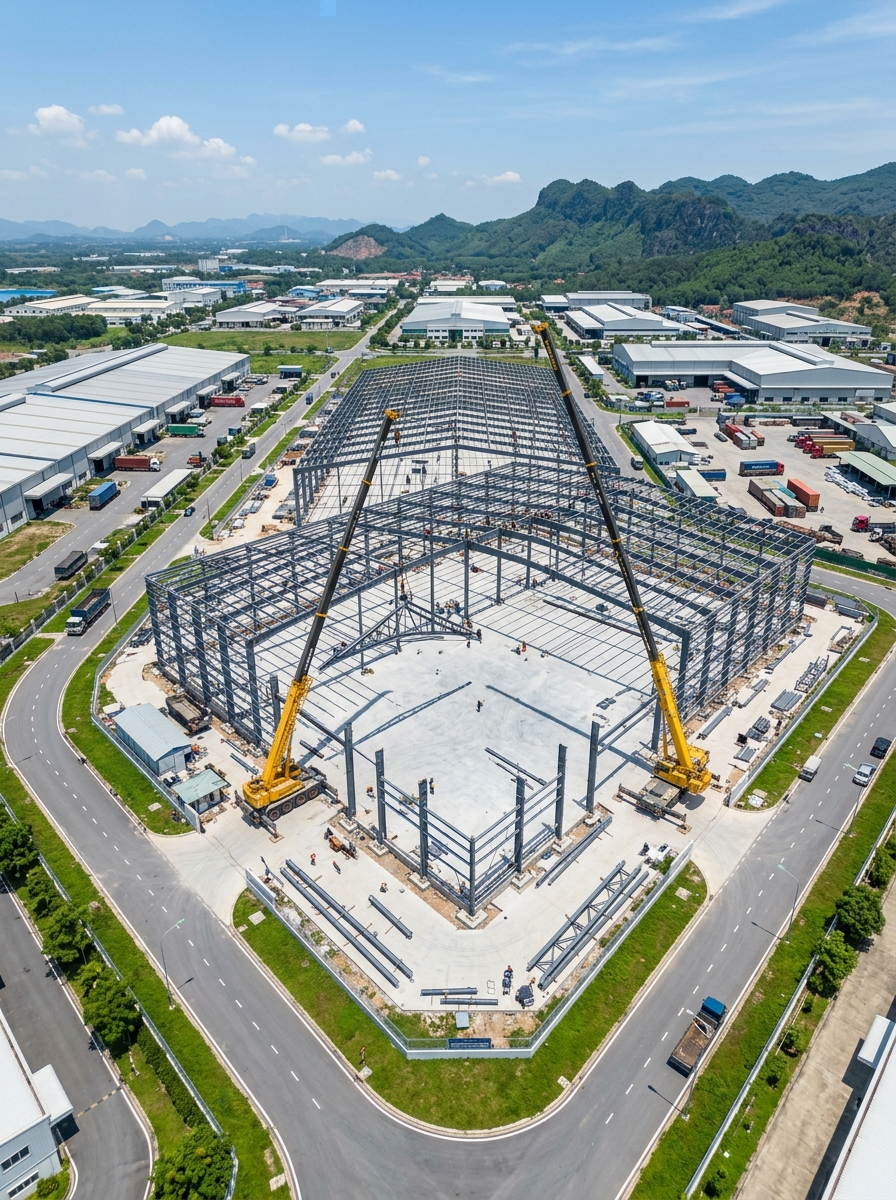
\includegraphics[height=\paperheight]{../../public/executive-cover-hero.jpg}
  };

  % 2. A dark-to-clear gradient protects the copy without hiding the construction image.
  \shade[
    left color=TTCDeepNavy!96!black,
    right color=transparent,
    opacity=0.70
  ] (current page.south west) rectangle (current page.north east);

  % 3. TTC recognition bar and compact logo lock-up.
  \fill[TTCRed] (current page.north west) rectangle ++(\paperwidth, -2.2mm);
  \node[anchor=north west, fill=white, fill opacity=0.96, text opacity=1,
        rounded corners=1.5pt, inner xsep=5mm, inner ysep=3.8mm]
    at ([xshift=15mm,yshift=-13mm]current page.north west) {
      
\includegraphics[width=48mm]{../../public/logo-ttc-removebg-DNXrVdJp.png}
    };
  \node[anchor=north east, text=white, inner sep=0pt] at ([xshift=-15mm,yshift=-15mm]current page.north east) {
    {\fontsize{8}{10}\selectfont\bfseries COMPANY PROFILE \;|\; 2026}
  };

  % 4. Large left-aligned title fills the visual centre; the clear right side shows the site.
  \node[anchor=west, align=left, text width=128mm, inner sep=0pt]
    at ([xshift=16mm,yshift=160mm]current page.south west) {
      {\fontsize{7.8}{9.6}\selectfont\bfseries\color{TTCRed} TAN THANH CONG TECHNOLOGY CONSTRUCTION JOINT STOCK COMPANY}\\[6mm]
      {\fontsize{43}{49}\selectfont\bfseries\color{white} HỒ SƠ}\\[-2mm]
      {\fontsize{43}{49}\selectfont\bfseries\color{white} NĂNG LỰC}\\[4mm]
      {\color{TTCRed}\rule{73mm}{2.8pt}}\\[5mm]
      {\fontsize{17}{20}\selectfont\bfseries\color{white} COMPANY PROFILE}\\[10mm]
      {\fontsize{14}{17}\selectfont\bfseries\color{white} TỔNG THẦU EPC CÔNG NGHIỆP\\THẾ HỆ MỚI}\\[3mm]
      {\fontsize{9.5}{12}\selectfont\color{white!88!gray} Turnkey Industrial EPC General Contractor}
    };

  % 5. Proof points: compact, scannable and placed above the contact footer.
  \node[anchor=south west, align=left, fill=TTCDeepNavy!92!black, fill opacity=0.84,
        text=white, text opacity=1, rounded corners=1.5pt, inner xsep=6mm, inner ysep=4mm]
    at ([xshift=15mm,yshift=31mm]current page.south west) {
      {\fontsize{12}{14}\selectfont\bfseries 150+ DỰ ÁN \qquad HẠNG II BXD \qquad ISO 9001 / 14001 / 45001}\\[1.2mm]
      {\fontsize{7}{8.5}\selectfont\color{white!82!gray}Năng lực tổng thầu công nghiệp đã được chứng minh tại hiện trường}
    };

  % 6. Legal identity stays quiet; the cover remains a visual statement.
  \node[anchor=south west, text=white, inner sep=0pt] at ([xshift=15mm,yshift=19mm]current page.south west) {
    {\fontsize{6.6}{8.2}\selectfont\bfseries CÔNG TY CỔ PHẦN CÔNG NGHỆ XÂY DỰNG TÂN THÀNH CÔNG}
  };

  % 7. Persistent contact footer.
  \fill[TTCDeepNavy!97!black] (current page.south west) rectangle ++(\paperwidth, 11mm);
  \fill[TTCRed] ([yshift=11mm]current page.south west) rectangle ++(\paperwidth, 1.2mm);
  \node[anchor=south, text=white, inner sep=0pt] at ([yshift=3.4mm]current page.south) {
    {\fontsize{6.8}{8.2}\selectfont
      \faPhone\ +84 976 447 766 \quad\textbullet\quad
      \faEnvelope\ info@tanthanhcongjsc.com \quad\textbullet\quad
      \faGlobe\ tanthanhcongjsc.com \quad\textbullet\quad
      \faAward\ NĂNG LỰC HẠNG II BXD}
  };
\end{tikzpicture}
\mbox{}% Anchor the overlay to a physical page before advancing to page 02.
\newpage

% ============================================================
% TRANG 02: MỤC LỤC ĐIỀU HƯỚNG & THÔNG TIN PHÁP NHÂN TÓM TẮT
% ============================================================
\pageheaderbar{MỤC LỤC \& THÔNG TIN PHÁP NHÂN}{Trang 02}
\pagefooterbar{Trang 02}

\begin{tikzpicture}[remember picture, overlay]
  \node[opacity=0.025, scale=4.2, font=\bfseries\sffamily, text=TTCBlue]
    at ([xshift=30mm,yshift=-8mm]current page.center) {TTC};
  \fill[TTCRed, opacity=0.05] ([xshift=12mm,yshift=18mm]current page.south west)
    rectangle ([xshift=18mm,yshift=248mm]current page.south west);
\end{tikzpicture}

\begin{minipage}[t][246mm]{\textwidth}
\secbrand{Mục Lục Tổng Quan}{Executive Contents — 06 Chuyên Mục Trọng Tâm}

{\fontsize{9.2}{11.5}\selectfont\color{TTCTextMuted}
Hồ sơ được tổ chức theo 06 nhóm năng lực để Chủ đầu tư tra cứu nhanh; chi tiết từng hạng mục được trình bày tại các trang chuyên đề.}\\[3mm]

% Navigation cards: inspired by section-based contents, without repeating every page title.
\newcommand{\toccard}[5]{%
  \begin{tikzpicture}
    \node[rounded corners=3pt, fill=white, draw=TTCBorder, line width=0.8pt,
          minimum width=90mm, minimum height=52mm, text width=79mm, inner sep=5.5mm, align=left] {
      {\fontsize{18}{19}\selectfont\bfseries\color{TTCRed} #1}\hspace{3mm}
      {\fontsize{8.2}{9.5}\selectfont\bfseries\color{TTCRed} TRANG #2}\\[1.5mm]
      {\fontsize{11.2}{13.2}\selectfont\bfseries\color{TTCBlue} #3}\\[0.3mm]
      {\fontsize{7.2}{8.8}\selectfont\itshape\color{TTCTextMuted} #4}\\[3mm]
      {\fontsize{8.2}{10.5}\selectfont\color{TTCTextDark} #5}
    };
  \end{tikzpicture}%
}

\noindent
\begin{tabular}{@{}p{91mm}@{\hspace{4mm}}p{91mm}@{}}
\toccard{I}{01--07}{GIỚI THIỆU \& NĂNG LỰC}{Company profile \& credentials}{Thư ngỏ \textbullet\ Tầm nhìn và giá trị \textbullet\ Hệ sinh thái \textbullet\ Pháp nhân \& lãnh đạo} &
\toccard{IV}{14--19}{GIẢI PHÁP EPC \& CÔNG NGHỆ}{EPC, ConTech \& ESG}{Fast-track EPC \textbullet\ BIM / AI \textbullet\ ESG \textbullet\ QA/QC \& HSE} \\[3.5mm]
\toccard{II}{08--10}{TÀI CHÍNH \& NHÂN SỰ}{Financial capacity \& people}{Doanh thu \textbullet\ Bảo lãnh tín dụng \textbullet\ Nguồn lực \textbullet\ Văn hóa an toàn} &
\toccard{V}{20--30}{DỰ ÁN \& KHÁCH HÀNG}{Projects \& valued partners}{Danh mục dự án \textbullet\ 06 case studies \textbullet\ Chuỗi cung ứng \textbullet\ Đối tác FDI} \\[3.5mm]
\toccard{III}{11--13}{SẢN XUẤT \& QUẢN TRỊ}{PEB \& project control}{Đối tác PEB \textbullet\ Thiết bị cơ giới \textbullet\ Quy trình quản trị FIDIC} &
\toccard{VI}{31--36}{CAM KẾT \& ĐỒNG HÀNH}{Commitments \& support}{Chứng nhận \textbullet\ Phủ sóng thi công \textbullet\ Chiến lược \textbullet\ Bảo hành \& liên hệ}
\end{tabular}

\vspace{4.5mm}

% Compact legal snapshot: details remain on the legal-credentials spread (page 06).
\noindent
\begin{tikzpicture}
  \node[rounded corners=3pt, fill=TTCLightBlue, draw=TTCBorder, line width=0.8pt,
        minimum width=186mm, text width=172mm, inner sep=7.5mm] {
    {\fontsize{10.5}{12.5}\selectfont\bfseries\color{TTCBlue} \faIdCard\quad HỒ SƠ PHÁP NHÂN TÓM TẮT}
    \hfill {\fontsize{7.2}{8.8}\selectfont\color{TTCRed}\bfseries CHI TIẾT CHỨNG NHẬN: TRANG 06}\\[1.5mm]
    {\fontsize{6.2}{7.5}\selectfont\color{TTCTextMuted}\bfseries
    TAN THANH CONG TECHNOLOGY CONSTRUCTION JOINT STOCK COMPANY}\\[3mm]
    \renewcommand{\arraystretch}{1.28}
    {\fontsize{8.2}{10.2}\selectfont
    \begin{tabularx}{\linewidth}{@{}p{32mm}X@{\hspace{5mm}}p{28mm}X@{}}
      \textbf{Tên doanh nghiệp} & \textbf{CÔNG TY CỔ PHẦN CÔNG NGHỆ XÂY DỰNG TÂN THÀNH CÔNG} &
      \textbf{Mã số thuế} & \textbf{0107090447} \\
      \textbf{Đại diện pháp luật} & \textbf{Ông PHẠM HUY TÂN} — Tổng Giám Đốc &
      \textbf{Năng lực} & Hạng II BXD \textbullet\ ISO 9001 / 14001 / 45001 \\
      \textbf{Trụ sở đăng ký} & Số 39, ngõ 292 Kim Giang, Đại Kim, Hà Nội &
      \textbf{Văn phòng giao dịch} & Số 19N7B, KĐT Trung Hòa Nhân Chính, Hà Nội \\
      \textbf{Liên hệ} & +84 976 447 766 \textbullet\ info@tanthanhcongjsc.com &
      \textbf{Website} & tanthanhcongjsc.com
    \end{tabularx}}
  };
\end{tikzpicture}
\end{minipage}
\newpage

% ============================================================
% TRANG 03: THÔNG ĐIỆP TỪ TỔNG GIÁM ĐỐC — LEADERSHIP MESSAGE
% ============================================================
\pageheaderbar{THÔNG ĐIỆP TỪ TỔNG GIÁM ĐỐC}{Trang 03}
\pagefooterbar{Trang 03}

\begin{tikzpicture}[remember picture, overlay]
  \node[opacity=0.025, scale=4.0, font=\bfseries\sffamily, text=TTCBlue]
    at ([xshift=-25mm,yshift=-25mm]current page.center) {LEADERSHIP};
  \fill[TTCRed, opacity=0.045] ([xshift=12mm,yshift=18mm]current page.south west)
    rectangle ([xshift=18mm,yshift=248mm]current page.south west);
\end{tikzpicture}

\begin{minipage}[t][246mm]{\textwidth}
\secbrand{Thông Điệp Từ Tổng Giám Đốc}{Leadership Message — Building Trust Through Every Commitment}

\vspace{2mm}

% Main editorial spread: concise letter on the left, authentic CEO portrait on the right.
\noindent
\begin{tabular}{@{}p{106mm}@{\hspace{4mm}}p{76mm}@{}}
  \begin{tikzpicture}
    \path[use as bounding box] (0,0) rectangle (106mm,170mm);
    \draw[TTCRed, line width=2.2pt] (0,169mm) -- (26mm,169mm);
    \node[anchor=north west, align=left, text width=98mm, inner sep=0pt] at (0,165mm) {
      {\fontsize{8.5}{10}\selectfont\bfseries\color{TTCRed} THÔNG ĐIỆP NHẤT QUÁN CỦA TTC}\\[4mm]
      {\fontsize{19}{23}\selectfont\bfseries\color{TTCBlue}
      ``CHẤT LƯỢNG LÀ DANH DỰ.\\
      AN TOÀN LÀ SINH MỆNH.\\
      TIẾN ĐỘ LÀ CAM KẾT.''}\\[6mm]
      {\fontsize{10}{12}\selectfont\bfseries\color{TTCBlue}
      Kính gửi Quý Chủ đầu tư, Quý Khách hàng và Quý Đối tác,}\\[3mm]
      {\fontsize{9.2}{13.2}\selectfont\color{TTCTextDark}
      Thay mặt Ban Lãnh đạo và toàn thể cán bộ công nhân viên \textbf{Công ty Cổ phần Công nghệ Xây dựng Tân Thành Công}, tôi trân trọng cảm ơn sự tin tưởng và đồng hành của Quý vị trong suốt chặng đường phát triển của TTC.\\[3mm]

      Hơn một thập kỷ hoạt động trong lĩnh vực xây dựng công nghiệp giúp chúng tôi thấu hiểu rằng: một dự án thành công phải đồng thời đáp ứng \textbf{chất lượng, an toàn, tiến độ và hiệu quả đầu tư}. Vì vậy, TTC kiên định với mô hình \textbf{Tổng thầu EPC một đầu mối}, kết hợp Value Engineering, BIM 5D và năng lực quản trị hiện trường theo tiêu chuẩn quốc tế.\\[3mm]

      Với hệ sinh thái đối tác PEB công suất 30.000 tấn/năm và đội ngũ kỹ sư thực chiến, chúng tôi cam kết cung cấp giải pháp phù hợp nhất cho từng nhà máy, kiểm soát minh bạch từ thiết kế, thi công đến bàn giao và bảo hành.\\[3mm]

      TTC mong muốn không chỉ là một nhà thầu, mà là \textbf{đối tác kiến tạo giá trị dài hạn} cùng Chủ đầu tư trên mỗi công trình.}\\[5mm]
      {\fontsize{9}{11}\selectfont\itshape\color{TTCTextMuted} Trân trọng,}
    };
  \end{tikzpicture}
  &
  \begin{tikzpicture}
    \path[use as bounding box] (0,0) rectangle (76mm,170mm);
    \fill[TTCLightBlue] (0,0) rectangle (76mm,170mm);
    \draw[TTCBorder, line width=0.8pt] (0,0) rectangle (76mm,170mm);
    \fill[TTCRed] (0,0) rectangle (3mm,170mm);

    \node[anchor=north, inner sep=0pt] at (39.5mm,168mm) {
      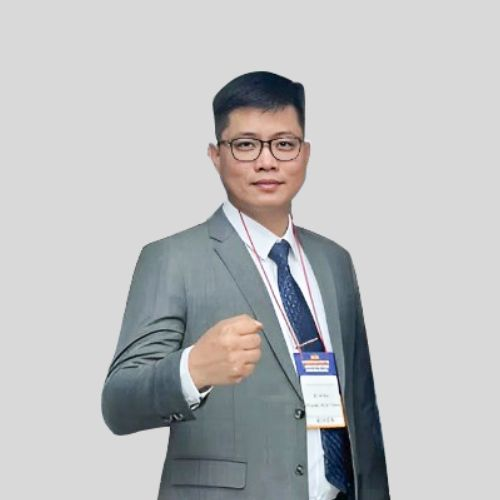
\includegraphics[trim=90 0 90 0,clip,height=116mm]{../tan_avatar.jpg}
    };

    \fill[TTCDeepNavy!97!black] (3mm,0) rectangle (76mm,54mm);
    \fill[TTCRed] (3mm,54mm) rectangle (76mm,56mm);
    \node[anchor=north west, align=left, text width=62mm, inner sep=0pt]
      at (10mm,46mm) {
        {\fontsize{7}{8.5}\selectfont\bfseries\color{TTCRed} TỔNG GIÁM ĐỐC / CEO}\\[2mm]
        {\fontsize{14}{17}\selectfont\bfseries\color{white} PHẠM HUY TÂN}\\[2mm]
        {\fontsize{7.5}{9.5}\selectfont\color{white!78!gray}
        Công ty Cổ phần Công nghệ\\Xây dựng Tân Thành Công}\\[4mm]
        {\fontsize{7.2}{9}\selectfont\bfseries\color{white!68!gray} TÂN THÀNH CÔNG \textbullet\ TTC JSC}
      };
  \end{tikzpicture}
\end{tabular}

\vspace{5mm}

% Three commitments replace the duplicated vision/mission content.
\noindent
\begin{tabular}{@{}p{58mm}@{\hspace{6mm}}p{58mm}@{\hspace{6mm}}p{58mm}@{}}
  \begin{tikzpicture}
    \node[rounded corners=3pt, fill=TTCDeepNavy!97!black, minimum width=58mm,
          minimum height=43mm, text width=48mm, align=center, inner sep=5mm] {
      {\fontsize{17}{19}\selectfont\bfseries\color{white} 01}\\[1mm]
      {\fontsize{9}{11}\selectfont\bfseries\color{TTCRed} ĐẦU MỐI EPC}\\[2mm]
      {\fontsize{7.3}{9}\selectfont\color{white!78!gray}Design \textbullet\ Build \textbullet\ Turnkey}
    };
  \end{tikzpicture}
  &
  \begin{tikzpicture}
    \node[rounded corners=3pt, fill=TTCLightBlue, draw=TTCBorder, line width=0.8pt,
          minimum width=58mm, minimum height=43mm, text width=48mm, align=center, inner sep=5mm] {
      {\fontsize{17}{19}\selectfont\bfseries\color{TTCRed} 10--15\%}\\[1mm]
      {\fontsize{9}{11}\selectfont\bfseries\color{TTCBlue} TỐI ƯU CHI PHÍ}\\[2mm]
      {\fontsize{7.3}{9}\selectfont\color{TTCTextMuted}Value Engineering}
    };
  \end{tikzpicture}
  &
  \begin{tikzpicture}
    \node[rounded corners=3pt, fill=TTCLightBlue, draw=TTCBorder, line width=0.8pt,
          minimum width=58mm, minimum height=43mm, text width=48mm, align=center, inner sep=5mm] {
      {\fontsize{15}{18}\selectfont\bfseries\color{TTCRed} ZERO}\\[1mm]
      {\fontsize{9}{11}\selectfont\bfseries\color{TTCBlue} ACCIDENT}\\[2mm]
      {\fontsize{7.3}{9}\selectfont\color{TTCTextMuted}HSE Commitment}
    };
  \end{tikzpicture}
\end{tabular}

\vspace{6mm}

\noindent
\begin{tikzpicture}
  \node[rounded corners=2pt, fill=white, draw=TTCRed, line width=0.9pt,
        minimum width=186mm, minimum height=15mm, align=center, inner sep=3mm] {
    {\fontsize{10}{12}\selectfont\bfseries\color{TTCBlue}
    KIẾN TẠO GIÁ TRỊ DÀI HẠN \quad\textbullet\quad BUILDING ENDURING VALUE}
  };
\end{tikzpicture}
\end{minipage}
\newpage

% ============================================================
% TRANG 04: KẾT CẤU VƯƠN CAO — HÀNH TRÌNH & GIÁ TRỊ CỐT LÕI
% ============================================================
\pageheaderbar{HÀNH TRÌNH PHÁT TRIỂN \& GIÁ TRỊ CỐT LÕI}{Trang 04}
\pagefooterbar{Trang 04}

\begin{tikzpicture}[remember picture, overlay]
  \node[opacity=0.022, scale=4.0, font=\bfseries\sffamily, text=TTCBlue]
    at ([xshift=15mm,yshift=-18mm]current page.center) {BUILDING THE FUTURE};
\end{tikzpicture}

\begin{minipage}[t][246mm]{\textwidth}
\secbrand{Hành Trình Kiến Tạo}{From Mechanical Foundations to a Next-Generation EPC General Contractor}

\vspace{1mm}

\noindent
\begin{tikzpicture}
  \node[anchor=west, align=left, inner sep=0pt] at (0,7mm) {
    {\fontsize{16}{19}\selectfont\bfseries\color{TTCBlue}
    TỪ NỀN TẢNG CƠ KHÍ ĐẾN TỔNG THẦU EPC THẾ HỆ MỚI}\\[1.5mm]
    {\fontsize{7.8}{9.5}\selectfont\color{TTCTextMuted}
    Một hành trình phát triển được nâng đỡ bởi năng lực thực thi, công nghệ và những giá trị bất biến.}
  };
  \fill[TTCRed] (0,0) rectangle (52mm,1.4mm);
\end{tikzpicture}

\vspace{3mm}

% Diagonal growth spine — a steel-beam metaphor for TTC's development.
\noindent
\begin{tikzpicture}[x=1mm,y=1mm]
  \path[use as bounding box] (0,0) rectangle (186,112);
  \fill[TTCLightBlue!55!white] (0,0) rectangle (186,112);
  \draw[TTCBorder, line width=0.8pt, rounded corners=3pt] (0,0) rectangle (186,112);
  \draw[TTCBlue!7!white, line width=0.35pt] (0,0) grid[step=10mm] (186,112);

  % Stepped structural spine: horizontal floor plates linked by rising steel members.
  \draw[TTCBlue!10!white, line width=7pt, line join=round]
    (16,19) -- (44,19) -- (52,40) -- (76,40) -- (84,61) --
    (116,61) -- (124,82) -- (155,82) -- (163,105) -- (180,105);
  \draw[TTCBlue!28!white, line width=1pt, line join=round]
    (12,14) -- (41,14) -- (49,35) -- (73,35) -- (81,56) --
    (113,56) -- (121,77) -- (152,77) -- (160,100) -- (177,100);
  \draw[TTCRed, line width=3.2pt, line join=round]
    (16,19) -- (44,19) -- (52,40) -- (76,40) -- (84,61) --
    (116,61) -- (124,82) -- (155,82) -- (163,105) -- (180,105);
  \draw[TTCRed, line width=1.1pt, -{Stealth[length=4mm]}] (180,105) -- (184,109);

  % 2015
  \fill[white] (16,19) circle (3.4);
  \draw[TTCRed, line width=1.5pt] (16,19) circle (3.4);
  \fill[TTCRed] (16,19) circle (1.35);
  \node[anchor=south west, align=left, text width=38mm, fill=TTCLightBlue!86!white,
        fill opacity=0.94, text opacity=1, rounded corners=1.5pt, inner sep=1mm] at (7,25) {
    {\fontsize{18}{20}\selectfont\bfseries\color{TTCRed} 2015}\\[-0.5mm]
    {\fontsize{8.5}{10}\selectfont\bfseries\color{TTCBlue} KHỞI TẠO}\\[1mm]
    {\fontsize{7.2}{9}\selectfont\color{TTCTextDark}Nền tảng cơ khí chính xác\\và kỹ thuật kết cấu thép.}
  };

  % 2018
  \fill[white] (55,40) circle (3.4);
  \draw[TTCRed, line width=1.5pt] (55,40) circle (3.4);
  \fill[TTCRed] (55,40) circle (1.35);
  \node[anchor=north west, align=left, text width=38mm, fill=TTCLightBlue!86!white,
        fill opacity=0.94, text opacity=1, rounded corners=1.5pt, inner sep=1mm] at (38,29) {
    {\fontsize{18}{20}\selectfont\bfseries\color{TTCRed} 2018}\\[-0.5mm]
    {\fontsize{8.5}{10}\selectfont\bfseries\color{TTCBlue} MỞ RỘNG}\\[1mm]
    {\fontsize{7.2}{9}\selectfont\color{TTCTextDark}Liên kết sản xuất PEB\\và tổng thầu hạ tầng KCN.}
  };

  % 2022
  \fill[white] (94,61) circle (3.4);
  \draw[TTCRed, line width=1.5pt] (94,61) circle (3.4);
  \fill[TTCRed] (94,61) circle (1.35);
  \node[anchor=south west, align=left, text width=39mm, fill=TTCLightBlue!86!white,
        fill opacity=0.94, text opacity=1, rounded corners=1.5pt, inner sep=1mm] at (71,67) {
    {\fontsize{18}{20}\selectfont\bfseries\color{TTCRed} 2022}\\[-0.5mm]
    {\fontsize{8.5}{10}\selectfont\bfseries\color{TTCBlue} BỨT PHÁ}\\[1mm]
    {\fontsize{7.2}{9}\selectfont\color{TTCTextDark}Hạng II Bộ Xây Dựng\\và các dự án FDI quy mô lớn.}
  };

  % 2026
  \fill[white] (134,82) circle (3.4);
  \draw[TTCRed, line width=1.5pt] (134,82) circle (3.4);
  \fill[TTCRed] (134,82) circle (1.35);
  \node[anchor=north west, align=left, text width=42mm, fill=TTCLightBlue!86!white,
        fill opacity=0.94, text opacity=1, rounded corners=1.5pt, inner sep=1mm] at (119,68) {
    {\fontsize{18}{20}\selectfont\bfseries\color{TTCRed} 2026}\\[-0.5mm]
    {\fontsize{8.5}{10}\selectfont\bfseries\color{TTCBlue} CHUYỂN ĐỔI}\\[1mm]
    {\fontsize{7.2}{9}\selectfont\color{TTCTextDark}150+ dự án \textbullet\ 20+ tỉnh thành\\PEB 30.000 tấn/năm.}
  };

  % 2030
  \fill[white] (176,105) circle (3.4);
  \draw[TTCRed, line width=1.5pt] (176,105) circle (3.4);
  \fill[TTCRed] (176,105) circle (1.35);
  \node[anchor=north east, align=right, text width=40mm, fill=TTCLightBlue!86!white,
        fill opacity=0.94, text opacity=1, rounded corners=1.5pt, inner sep=1mm] at (178,98) {
    {\fontsize{18}{20}\selectfont\bfseries\color{TTCRed} 2030}\\[-0.5mm]
    {\fontsize{8.5}{10}\selectfont\bfseries\color{TTCBlue} VƯƠN TẦM}\\[1mm]
    {\fontsize{7.2}{9}\selectfont\color{TTCTextDark}ConTech \textbullet\ ESG\\Mở rộng Đông Nam Á.}
  };
\end{tikzpicture}

\vspace{4mm}

% Photo foundation: five core values become the structural base of the journey.
\noindent
\begin{tikzpicture}[x=1mm,y=1mm]
  \path[use as bounding box] (0,0) rectangle (186,112);
  \clip[rounded corners=3pt] (0,0) rectangle (186,112);
  \node[anchor=center, inner sep=0pt] at (93,56) {
    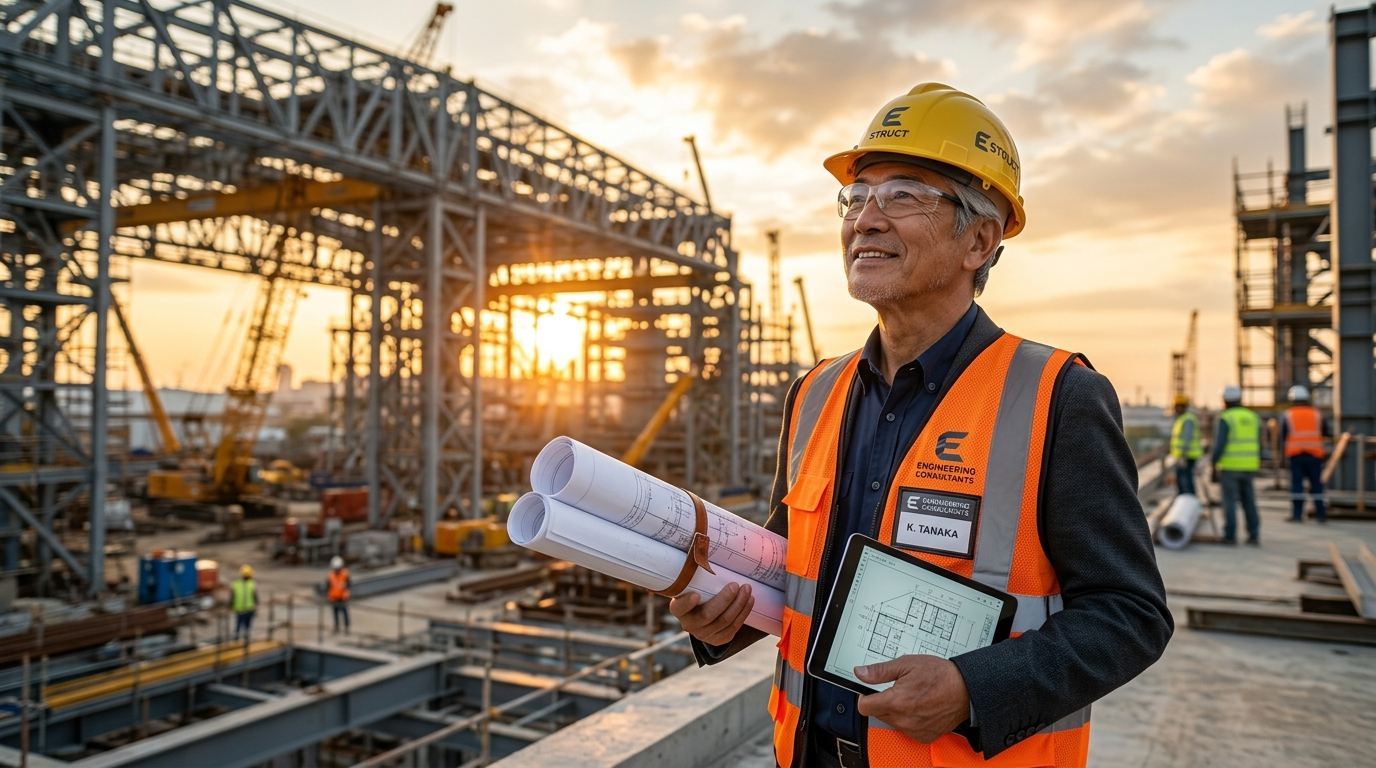
\includegraphics[height=112mm]{assets/milestones_engineer_hero.jpg}
  };
  \shade[left color=TTCDeepNavy!98!black, right color=transparent, opacity=0.82]
    (0,31) rectangle (142,112);
  \node[anchor=north west, align=left, text width=112mm, inner sep=0pt] at (8,104) {
    {\fontsize{12}{14}\selectfont\bfseries\color{white}5 GIÁ TRỊ — NỀN MÓNG CỦA MỌI CÔNG TRÌNH}\\[1.5mm]
    {\fontsize{7.5}{9}\selectfont\color{white!82!gray}The values that sustain every commitment and every project.}
  };

  \fill[TTCDeepNavy!97!black, opacity=0.96] (0,0) rectangle (37.2,31);
  \fill[TTCDeepNavy!91!black, opacity=0.96] (37.2,0) rectangle (74.4,31);
  \fill[TTCDeepNavy!97!black, opacity=0.96] (74.4,0) rectangle (111.6,31);
  \fill[TTCDeepNavy!91!black, opacity=0.96] (111.6,0) rectangle (148.8,31);
  \fill[TTCDeepNavy!97!black, opacity=0.96] (148.8,0) rectangle (186,31);
  \fill[TTCRed] (0,31) rectangle (186,32.3);

  \node[align=center, text=white] at (18.6,15.5) {
    {\fontsize{14}{16}\selectfont\bfseries TÍN}\\[1mm]
    {\fontsize{6.8}{8}\selectfont\color{white!72!gray}TRUST \& INTEGRITY}
  };
  \node[align=center, text=white] at (55.8,15.5) {
    {\fontsize{14}{16}\selectfont\bfseries TÂM}\\[1mm]
    {\fontsize{6.8}{8}\selectfont\color{white!72!gray}DEDICATION}
  };
  \node[align=center, text=white] at (93,15.5) {
    {\fontsize{14}{16}\selectfont\bfseries TRÍ}\\[1mm]
    {\fontsize{6.8}{8}\selectfont\color{white!72!gray}INNOVATION}
  };
  \node[align=center, text=white] at (130.2,15.5) {
    {\fontsize{14}{16}\selectfont\bfseries TỐC}\\[1mm]
    {\fontsize{6.8}{8}\selectfont\color{white!72!gray}FAST-TRACK}
  };
  \node[align=center, text=white] at (167.4,15.5) {
    {\fontsize{14}{16}\selectfont\bfseries AN}\\[1mm]
    {\fontsize{6.8}{8}\selectfont\color{white!72!gray}HSE \& SAFETY}
  };
\end{tikzpicture}
\end{minipage}
\newpage

% ============================================================
% TRANG 05: INTEGRATED FACTORY BLUEPRINT
% ============================================================
\pageheaderbar{HỆ SINH THÁI TỔNG THẦU EPC \& R\&D CÔNG NGHỆ}{Trang 05}
\pagefooterbar{Trang 05}

\begin{tikzpicture}[remember picture, overlay]
  \draw[TTCBlue!6!white, line width=0.45pt]
    ([xshift=15mm,yshift=18mm]current page.south west)
    grid[step=8mm]
    ([xshift=195mm,yshift=42mm]current page.south west);
\end{tikzpicture}

\begin{minipage}[t][246mm]{\textwidth}
\secbrand{Hệ Sinh Thái Tổng Thầu EPC}{Integrated Factory Blueprint \& AIDC ConTech Collaboration}

\vspace{1mm}
{\fontsize{15}{17}\selectfont\bfseries\color{TTCBlue}
MỘT HỆ SINH THÁI • MỘT HỢP ĐỒNG • MỘT TRÁCH NHIỆM\par}
\vspace{1mm}
{\fontsize{7.5}{9}\selectfont\color{TTCTextMuted}
One integrated ecosystem. One accountable EPC partner from concept to handover.\par}
\vspace{3mm}

% HERO: NHÀ MÁY LÀ TRUNG TÂM, NĂNG LỰC LÀ CÁC LỚP TÍCH HỢP
\noindent
\begin{tikzpicture}[x=1mm,y=1mm]
  \path[use as bounding box] (0,0) rectangle (186,118);
  \clip[rounded corners=3pt] (0,0) rectangle (186,118);
  \node[anchor=center, inner sep=0pt] at (93,59)
    {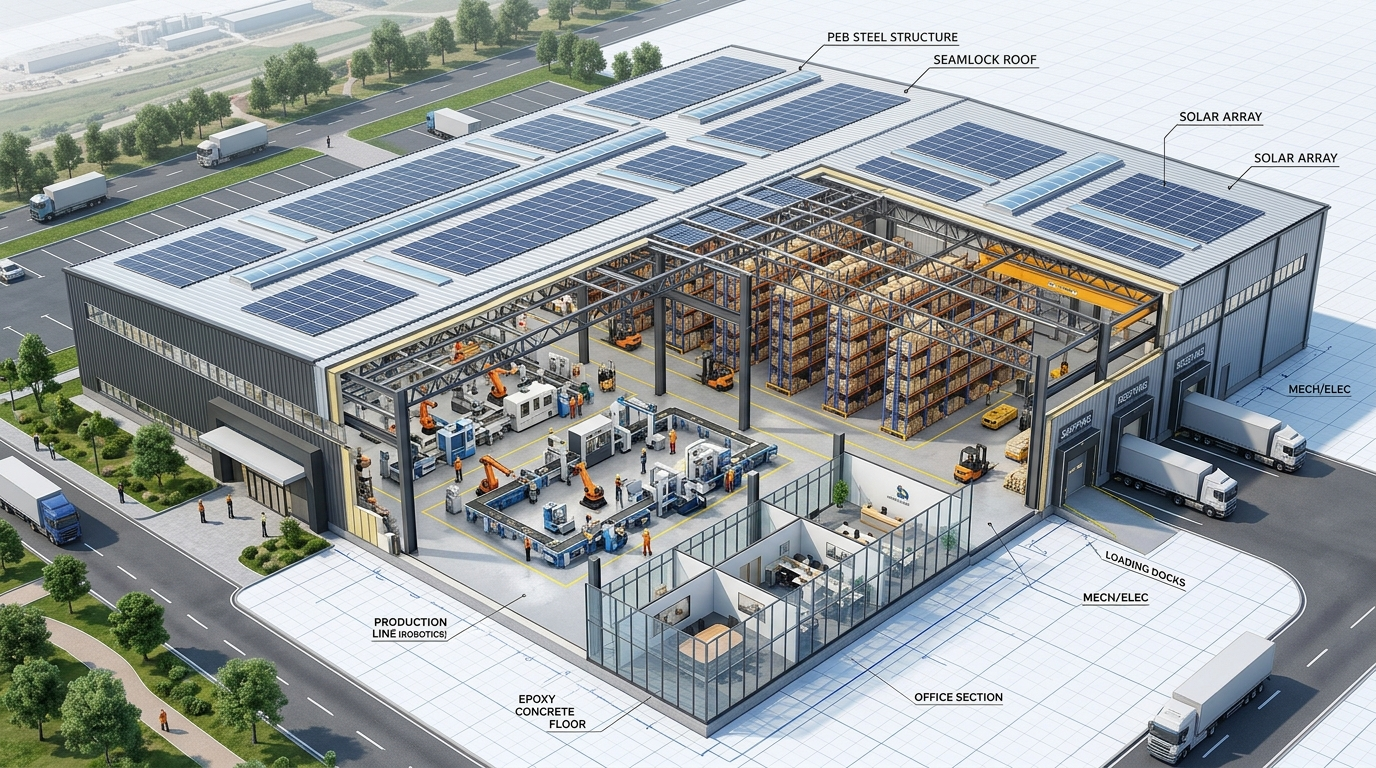
\includegraphics[height=118mm]{../../public/factory-tech-3d.jpg}};
  \fill[white, opacity=0.10] (0,0) rectangle (186,118);

  % Connectors — thin and quiet
  \draw[TTCBlue!55!white, line width=0.65pt] (55,91) -- (80,72);
  \draw[TTCBlue!55!white, line width=0.65pt] (55,38) -- (81,57);
  \draw[TTCBlue!55!white, line width=0.65pt] (131,91) -- (107,72);
  \draw[TTCRed!72!white, line width=0.75pt] (131,38) -- (106,57);

  % 01 — AIDC ConTech
  \node[
    anchor=north west, rounded corners=3pt,
    fill=white, fill opacity=0.94, text opacity=1,
    draw=TTCCyan!70!white, line width=0.65pt,
    minimum width=53mm, minimum height=29mm,
    text width=47mm, inner sep=3mm, align=left
  ] at (5,113) {
    {\fontsize{7.3}{8.5}\selectfont\bfseries\color{TTCCyan} 01 / AIDC CONTECH}\\[1mm]
    {\fontsize{10}{11.5}\selectfont\bfseries\color{TTCBlue} BIM 5D • AI • VALUE ENGINEERING}\\[1mm]
    {\fontsize{7}{8.6}\selectfont\color{TTCTextDark}Tối ưu thiết kế và dữ liệu dự án; tiết kiệm 10--15\% chi phí đầu tư.}
  };

  % 02 — MEP & PCCC
  \node[
    anchor=south west, rounded corners=3pt,
    fill=white, fill opacity=0.94, text opacity=1,
    draw=TTCBlue!42!white, line width=0.65pt,
    minimum width=53mm, minimum height=29mm,
    text width=47mm, inner sep=3mm, align=left
  ] at (5,5) {
    {\fontsize{7.3}{8.5}\selectfont\bfseries\color{TTCBlue} 02 / MEP \& PCCC}\\[1mm]
    {\fontsize{10}{11.5}\selectfont\bfseries\color{TTCBlue} HỆ THỐNG ĐỒNG BỘ TRÊN BIM}\\[1mm]
    {\fontsize{7}{8.6}\selectfont\color{TTCTextDark}Điện • HVAC • cấp thoát nước • phòng cháy, phối hợp xuyên suốt một mô hình.}
  };

  % 03 — Hạ tầng
  \node[
    anchor=north east, rounded corners=3pt,
    fill=white, fill opacity=0.94, text opacity=1,
    draw=TTCBlue!42!white, line width=0.65pt,
    minimum width=53mm, minimum height=29mm,
    text width=47mm, inner sep=3mm, align=left
  ] at (181,113) {
    {\fontsize{7.3}{8.5}\selectfont\bfseries\color{TTCBlue} 03 / HẠ TẦNG KCN}\\[1mm]
    {\fontsize{10}{11.5}\selectfont\bfseries\color{TTCBlue} NỀN MÓNG • ĐƯỜNG • THOÁT NƯỚC}\\[1mm]
    {\fontsize{7}{8.6}\selectfont\color{TTCTextDark}Hạ tầng kỹ thuật sẵn sàng vận hành, kết nối đồng bộ với tổng mặt bằng nhà máy.}
  };

  % 04 — PEB LAST
  \node[
    anchor=south east, rounded corners=3pt,
    fill=white, fill opacity=0.96, text opacity=1,
    draw=TTCRed!78!white, line width=0.8pt,
    minimum width=53mm, minimum height=29mm,
    text width=47mm, inner sep=3mm, align=left
  ] at (181,5) {
    {\fontsize{7.3}{8.5}\selectfont\bfseries\color{TTCRed} 04 / PEB MANUFACTURING}\\[1mm]
    {\fontsize{10}{11.5}\selectfont\bfseries\color{TTCBlue} SẢN XUẤT KẾT CẤU THÉP}\\[1mm]
    {\fontsize{7}{8.6}\selectfont\color{TTCTextDark}CNC • SAW • AWS D1.1 • NDT; năng lực cung ứng 30.000 tấn/năm.}
  };

  % Central accountability hub
  \node[
    rounded corners=3pt, fill=TTCDeepNavy!96!black,
    draw=TTCCyan!75!white, line width=0.9pt,
    minimum width=50mm, minimum height=28mm,
    text=white, align=center, inner sep=2.5mm
  ] at (93,64) {
    {\fontsize{11}{12.5}\selectfont\bfseries TÂN THÀNH CÔNG}\\[1mm]
    {\fontsize{7.5}{9}\selectfont\bfseries\color{TTCCyan} EPC SYSTEM INTEGRATOR}\\[1mm]
    {\fontsize{6.8}{8}\selectfont\color{white!78!gray}One contract • One accountability}
  };

  \draw[white, line width=1.2pt, rounded corners=3pt] (0.6,0.6) rectangle (185.4,117.4);
  \draw[TTCBorder, line width=0.65pt, rounded corners=3pt] (0,0) rectangle (186,118);
\end{tikzpicture}

\vspace{3mm}

% DELIVERY FLOW — PEB NẰM CUỐI TRONG CHUỖI NĂNG LỰC
\noindent
\begin{tikzpicture}[x=1mm,y=1mm]
  \path[use as bounding box] (0,0) rectangle (186,31);
  \fill[TTCLightBlue, rounded corners=4pt] (0,0) rectangle (186,31);
  \draw[TTCBorder, line width=0.65pt, rounded corners=4pt] (0,0) rectangle (186,31);

  \node[align=center] at (18,15.5) {
    {\fontsize{7}{8}\selectfont\bfseries\color{TTCTextMuted} 01}\\[0.7mm]
    {\fontsize{9.2}{10.5}\selectfont\bfseries\color{TTCBlue} KHẢO SÁT}\\[0.7mm]
    {\fontsize{6.6}{8}\selectfont Hiện trạng \& yêu cầu}
  };
  \node[align=center] at (55.5,15.5) {
    {\fontsize{7}{8}\selectfont\bfseries\color{TTCTextMuted} 02}\\[0.7mm]
    {\fontsize{9.2}{10.5}\selectfont\bfseries\color{TTCBlue} THIẾT KẾ}\\[0.7mm]
    {\fontsize{6.6}{8}\selectfont BIM • AI • VE}
  };
  \node[align=center] at (93,15.5) {
    {\fontsize{7}{8}\selectfont\bfseries\color{TTCTextMuted} 03}\\[0.7mm]
    {\fontsize{9.2}{10.5}\selectfont\bfseries\color{TTCBlue} HẠ TẦNG}\\[0.7mm]
    {\fontsize{6.6}{8}\selectfont Nền móng • tiện ích}
  };
  \node[align=center] at (130.5,15.5) {
    {\fontsize{7}{8}\selectfont\bfseries\color{TTCTextMuted} 04}\\[0.7mm]
    {\fontsize{9.2}{10.5}\selectfont\bfseries\color{TTCBlue} MEP \& PCCC}\\[0.7mm]
    {\fontsize{6.6}{8}\selectfont Tích hợp hệ thống}
  };
  \node[align=center] at (168,15.5) {
    {\fontsize{7}{8}\selectfont\bfseries\color{TTCRed} 05}\\[0.7mm]
    {\fontsize{9.2}{10.5}\selectfont\bfseries\color{TTCRed} PEB}\\[0.7mm]
    {\fontsize{6.6}{8}\selectfont Sản xuất • lắp dựng}
  };

  \foreach \x in {36.75,74.25,111.75,149.25}{
    \node[text=TTCRed, font=\fontsize{8}{9}\selectfont] at (\x,15.5) {\faChevronRight};
  }
\end{tikzpicture}

\vspace{3mm}

% THREE BUSINESS OUTCOMES — LIGHTER THAN THE OLD DARK KPI BAND
\noindent
\begin{tabular}{@{}p{58mm}@{\hspace{6mm}}p{58mm}@{\hspace{6mm}}p{58mm}@{}}
  \begin{tikzpicture}
    \node[
      rounded corners=4pt, fill=white, draw=TTCBorder,
      line width=0.65pt, minimum width=58mm, minimum height=35mm,
      text width=50mm, inner sep=4mm, align=left
    ] {
      {\fontsize{7}{8}\selectfont\bfseries\color{TTCRed} 01 / ACCOUNTABILITY}\\[1mm]
      {\fontsize{14}{15.5}\selectfont\bfseries\color{TTCBlue} 01 ĐẦU MỐI}\\[1mm]
      {\fontsize{7}{8.5}\selectfont\color{TTCTextDark}Một tổng thầu chịu trách nhiệm xuyên suốt từ thiết kế đến bàn giao.}
    };
  \end{tikzpicture}
  &
  \begin{tikzpicture}
    \node[
      rounded corners=4pt, fill=white, draw=TTCBorder,
      line width=0.65pt, minimum width=58mm, minimum height=35mm,
      text width=50mm, inner sep=4mm, align=left
    ] {
      {\fontsize{7}{8}\selectfont\bfseries\color{TTCCyan} 02 / OPTIMIZATION}\\[1mm]
      {\fontsize{14}{15.5}\selectfont\bfseries\color{TTCBlue} TỐI ƯU CHI PHÍ}\\[1mm]
      {\fontsize{7}{8.5}\selectfont\color{TTCTextDark}AI và Value Engineering tối ưu giải pháp kỹ thuật, tiết kiệm 10--15\% chi phí đầu tư.}
    };
  \end{tikzpicture}
  &
  \begin{tikzpicture}
    \node[
      rounded corners=4pt, fill=white, draw=TTCBorder,
      line width=0.65pt, minimum width=58mm, minimum height=35mm,
      text width=50mm, inner sep=4mm, align=left
    ] {
      {\fontsize{7}{8}\selectfont\bfseries\color{TTCBlue} 03 / INTEGRATION}\\[1mm]
      {\fontsize{14}{15.5}\selectfont\bfseries\color{TTCBlue} 100\% KHÉP KÍN}\\[1mm]
      {\fontsize{7}{8.5}\selectfont\color{TTCTextDark}Dữ liệu, kỹ thuật và thi công cùng vận hành trong một hệ sinh thái.}
    };
  \end{tikzpicture}
\end{tabular}

\vspace{3mm}

% TRUST STRIP — INTERNATIONAL CONTROL STANDARDS
\noindent
\begin{tikzpicture}[x=1mm,y=1mm]
  \path[use as bounding box] (0,0) rectangle (186,24);
  \fill[white, rounded corners=4pt] (0,0) rectangle (186,24);
  \draw[TTCBorder, line width=0.65pt, rounded corners=4pt] (0,0) rectangle (186,24);
  \fill[TTCLightBlue, rounded corners=4pt] (0,0) rectangle (43,24);
  \draw[TTCBorder, line width=0.55pt] (43,3) -- (43,21);

  \node[anchor=west, align=left] at (5,12) {
    {\fontsize{7}{8}\selectfont\bfseries\color{TTCCyan} DELIVERY ASSURANCE}\\[0.8mm]
    {\fontsize{9}{10.5}\selectfont\bfseries\color{TTCBlue} NỀN TẢNG KIỂM SOÁT}\\[0.6mm]
    {\fontsize{6.4}{7.8}\selectfont\color{TTCTextMuted} Standards behind every project}
  };
  \node[align=center] at (61,12) {
    {\fontsize{11}{12.5}\selectfont\bfseries\color{TTCBlue} ISO 9001}\\[0.8mm]
    {\fontsize{6.5}{8}\selectfont\color{TTCTextMuted} Quality}
  };
  \node[align=center] at (94,12) {
    {\fontsize{11}{12.5}\selectfont\bfseries\color{TTCBlue} ISO 14001}\\[0.8mm]
    {\fontsize{6.5}{8}\selectfont\color{TTCTextMuted} Environment}
  };
  \node[align=center] at (130,12) {
    {\fontsize{11}{12.5}\selectfont\bfseries\color{TTCBlue} ISO 45001}\\[0.8mm]
    {\fontsize{6.5}{8}\selectfont\color{TTCTextMuted} Health \& Safety}
  };
  \node[align=center] at (167,12) {
    {\fontsize{11}{12.5}\selectfont\bfseries\color{TTCRed} HẠNG II}\\[0.8mm]
    {\fontsize{6.5}{8}\selectfont\color{TTCTextMuted} Bộ Xây Dựng}
  };
\end{tikzpicture}
\end{minipage}
\newpage

% ============================================================
% TRANG 06: GOVERNANCE & COMPLIANCE DASHBOARD
% ============================================================
\pageheaderbar{CƠ CẤU TỔ CHỨC \& PHÁP LÝ HẠNG II BXD}{Trang 06}
\pagefooterbar{Trang 06}

\begin{tikzpicture}[remember picture, overlay]
  \draw[TTCBlue!6!white, line width=0.45pt]
    ([xshift=15mm,yshift=18mm]current page.south west)
    grid[step=8mm]
    ([xshift=195mm,yshift=42mm]current page.south west);
\end{tikzpicture}

\begin{minipage}[t][246mm]{\textwidth}
\secbrand{Quản Trị Tinh Gọn \& Nền Tảng Tuân Thủ}{Governance Structure, Grade II Construction License \& International ISO Systems}

\vspace{1mm}
{\fontsize{15}{17}\selectfont\bfseries\color{TTCBlue}
QUYỀN HẠN RÕ RÀNG • TRÁCH NHIỆM XUYÊN SUỐT DỰ ÁN\par}
\vspace{1mm}
{\fontsize{7.5}{9}\selectfont\color{TTCTextMuted}
An execution-led governance model connecting board oversight directly to every project site.\par}
\vspace{3mm}

% GOVERNANCE MAP
\noindent
\begin{tikzpicture}[x=1mm,y=1mm]
  \path[use as bounding box] (0,0) rectangle (186,105);
  \fill[white, rounded corners=4pt] (0,0) rectangle (186,105);
  \draw[TTCBorder, line width=0.7pt, rounded corners=4pt] (0,0) rectangle (186,105);

  \node[anchor=west, align=left] at (6,99) {
    {\fontsize{7}{8}\selectfont\bfseries\color{TTCCyan} DELIVERY GOVERNANCE}\\[-0.2mm]
    {\fontsize{9.5}{11}\selectfont\bfseries\color{TTCBlue} CẤU TRÚC ĐIỀU HÀNH THEO DÒNG TRÁCH NHIỆM}
  };
  \draw[TTCBorder, line width=0.5pt] (6,91.5) -- (180,91.5);

  % Connector architecture, drawn behind nodes
  \draw[TTCBlue!65!white, line width=0.75pt] (93,83) -- (93,75);
  \draw[TTCBlue!65!white, line width=0.75pt] (93,66) -- (93,61);
  \draw[TTCBlue!65!white, line width=0.75pt] (32,61) -- (154,61);
  \draw[TTCBlue!65!white, line width=0.75pt] (32,61) -- (32,57);
  \draw[TTCBlue!65!white, line width=0.75pt] (93,61) -- (93,57);
  \draw[TTCBlue!65!white, line width=0.75pt] (154,61) -- (154,57);
  \draw[TTCBlue!65!white, line width=0.75pt] (32,48) -- (32,43);
  \draw[TTCBlue!65!white, line width=0.75pt] (93,48) -- (93,43);
  \draw[TTCBlue!65!white, line width=0.75pt] (154,48) -- (154,43);
  \draw[TTCBlue!55!white, line width=0.65pt] (32,21) -- (32,16);
  \draw[TTCBlue!55!white, line width=0.65pt] (93,21) -- (93,16);
  \draw[TTCBlue!55!white, line width=0.65pt] (154,21) -- (154,16);
  \draw[TTCBlue!55!white, line width=0.65pt] (32,16) -- (154,16);
  \draw[TTCBlue!55!white, line width=0.65pt] (93,16) -- (93,13);
  \draw[TTCBlue!42!white, line width=0.6pt, dashed] (46,70.5) -- (62,70.5);
  \draw[TTCCyan!80!white, line width=0.6pt, dashed] (124,70.5) -- (140,70.5);

  % Board & executive leadership
  \node[
    rounded corners=3pt, fill=TTCDeepNavy, text=white,
    minimum width=78mm, minimum height=10mm, align=center
  ] at (93,83) {
    {\fontsize{7.8}{9.2}\selectfont\bfseries
    \faUsers\quad ĐẠI HỘI ĐỒNG CỔ ĐÔNG \& HỘI ĐỒNG QUẢN TRỊ}
  };
  \node[
    rounded corners=3pt, fill=TTCLightBlue, draw=TTCBorder,
    minimum width=42mm, minimum height=9mm, align=center
  ] at (25,70.5) {
    {\fontsize{7}{8.3}\selectfont\bfseries\color{TTCBlue} HỘI ĐỒNG CỐ VẤN QUỐC TẾ}
  };
  \node[
    rounded corners=3pt, fill=TTCRed, text=white,
    minimum width=62mm, minimum height=11mm, align=center
  ] at (93,70.5) {
    {\fontsize{8.2}{9.5}\selectfont\bfseries
    \faUserTie\quad TỔNG GIÁM ĐỐC}\\[0.5mm]
    {\fontsize{6.7}{8}\selectfont Ông PHẠM HUY TÂN}
  };
  \node[
    rounded corners=3pt, fill=TTCLightBlue, draw=TTCCyan,
    minimum width=42mm, minimum height=9mm, align=center
  ] at (161,70.5) {
    {\fontsize{7}{8.3}\selectfont\bfseries\color{TTCBlue}
    \faMicrochip\quad R\&D CÔNG NGHỆ AIDC}
  };

  % Three accountable executive streams
  \node[
    rounded corners=3pt, fill=TTCBlue, text=white,
    minimum width=54mm, minimum height=10mm, align=center
  ] at (32,52.5) {
    {\fontsize{7.4}{8.8}\selectfont\bfseries P.TGĐ DỰ ÁN \& THI CÔNG}
  };
  \node[
    rounded corners=3pt, fill=TTCBlue, text=white,
    minimum width=54mm, minimum height=10mm, align=center
  ] at (93,52.5) {
    {\fontsize{7.4}{8.8}\selectfont\bfseries P.TGĐ KỸ THUẬT \& BIM}
  };
  \node[
    rounded corners=3pt, fill=TTCBlue, text=white,
    minimum width=54mm, minimum height=10mm, align=center
  ] at (154,52.5) {
    {\fontsize{7.4}{8.8}\selectfont\bfseries P.TGĐ TÀI CHÍNH \& FIDIC}
  };

  % Functional teams
  \node[
    rounded corners=3pt, fill=white, draw=TTCBorder,
    minimum width=54mm, minimum height=22mm,
    text width=47mm, inner sep=3mm, align=left
  ] at (32,32) {
    {\fontsize{7.1}{8.4}\selectfont\bfseries\color{TTCBlue}\faHardHat\ PROJECT DELIVERY}\\[1mm]
    {\fontsize{6.7}{8.2}\selectfont\color{TTCTextDark}
    • Ban điều hành dự án FDI\\
    • Quản lý thi công \& cơ giới\\
    • HSE \& QA/QC hiện trường}
  };
  \node[
    rounded corners=3pt, fill=white, draw=TTCBorder,
    minimum width=54mm, minimum height=22mm,
    text width=47mm, inner sep=3mm, align=left
  ] at (93,32) {
    {\fontsize{7.1}{8.4}\selectfont\bfseries\color{TTCBlue}\faDraftingCompass\ ENGINEERING}\\[1mm]
    {\fontsize{6.7}{8.2}\selectfont\color{TTCTextDark}
    • Value Engineering \& kết cấu\\
    • BIM 5D \& quản trị dữ liệu\\
    • Quy hoạch, pháp lý \& PCCC}
  };
  \node[
    rounded corners=3pt, fill=white, draw=TTCBorder,
    minimum width=54mm, minimum height=22mm,
    text width=47mm, inner sep=3mm, align=left
  ] at (154,32) {
    {\fontsize{7.1}{8.4}\selectfont\bfseries\color{TTCBlue}\faFileInvoiceDollar\ COMMERCIAL}\\[1mm]
    {\fontsize{6.7}{8.2}\selectfont\color{TTCTextDark}
    • Đấu thầu \& hợp đồng FIDIC\\
    • Tài chính \& dòng tiền EPC\\
    • Chuỗi cung ứng Tier-1}
  };

  % Site execution layer
  \node[
    rounded corners=3pt, fill=TTCDeepNavy, draw=TTCCyan,
    line width=0.75pt, text=white,
    minimum width=174mm, minimum height=12mm, align=center
  ] at (93,8) {
    {\fontsize{7.7}{9}\selectfont\bfseries\color{TTCCyan}
    \faHardHat\quad BAN CHỈ HUY CÔNG TRƯỜNG — QUYỀN HẠN TẠI ĐIỂM THỰC THI}\\[0.6mm]
    {\fontsize{6.5}{7.8}\selectfont\color{white!82!gray}
    Chỉ huy trưởng Hạng II • Kỹ sư kết cấu • MEP • HSE • QA/QC thường trú}
  };
\end{tikzpicture}

\vspace{3mm}

% COMPLIANCE PASSPORT
\noindent
\begin{tikzpicture}[x=1mm,y=1mm]
  \path[use as bounding box] (0,0) rectangle (186,72);
  \fill[TTCLightBlue, rounded corners=4pt] (0,0) rectangle (186,72);
  \draw[TTCBorder, line width=0.7pt, rounded corners=4pt] (0,0) rectangle (186,72);

  \node[anchor=west, align=left] at (6,66) {
    {\fontsize{7}{8}\selectfont\bfseries\color{TTCCyan} COMPLIANCE PASSPORT}\\[-0.2mm]
    {\fontsize{9.5}{11}\selectfont\bfseries\color{TTCBlue}
    NĂNG LỰC PHÁP LÝ \& HỆ THỐNG QUẢN LÝ ĐƯỢC KIỂM CHỨNG}
  };

  % Grade II anchor card
  \fill[white, rounded corners=3pt] (5,7) rectangle (58,57);
  \draw[TTCRed, line width=0.9pt, rounded corners=3pt] (5,7) rectangle (58,57);
  \node[align=center] at (31.5,45) {
    {\fontsize{7}{8}\selectfont\bfseries\color{TTCRed} CONSTRUCTION LICENSE}\\[1mm]
    {\fontsize{22}{24}\selectfont\bfseries\color{TTCRed} HẠNG II}\\[-0.2mm]
    {\fontsize{9}{10.5}\selectfont\bfseries\color{TTCBlue} BỘ XÂY DỰNG}
  };
  \draw[TTCBorder, line width=0.5pt] (11,29) -- (52,29);
  \node[text width=42mm, align=left] at (31.5,18) {
    {\fontsize{6.6}{8.2}\selectfont\color{TTCTextDark}
    \textcolor{TTCRed}{\faCheckCircle}\ Tổng thầu thiết kế \& thi công\\
    \textcolor{TTCRed}{\faCheckCircle}\ Công trình công nghiệp quy mô lớn\\
    \textcolor{TTCRed}{\faCheckCircle}\ Kết cấu vượt nhịp lớn}
  };

  % ISO 9001
  \fill[white, rounded corners=3pt] (62,7) rectangle (100,57);
  \draw[TTCBorder, line width=0.6pt, rounded corners=3pt] (62,7) rectangle (100,57);
  \node[align=center] at (81,45) {
    {\fontsize{7}{8}\selectfont\bfseries\color{TTCCyan} QUALITY}\\[1mm]
    {\fontsize{13}{14.5}\selectfont\bfseries\color{TTCBlue} ISO 9001}\\
    {\fontsize{7}{8.5}\selectfont\bfseries\color{TTCTextMuted} 2015}
  };
  \node[text width=30mm, align=center] at (81,20) {
    {\fontsize{6.6}{8.2}\selectfont\color{TTCTextDark}
    Kiểm soát thiết kế, vật tư, thi công và nghiệm thu theo ITP.}
  };

  % ISO 14001
  \fill[white, rounded corners=3pt] (103,7) rectangle (141,57);
  \draw[TTCBorder, line width=0.6pt, rounded corners=3pt] (103,7) rectangle (141,57);
  \node[align=center] at (122,45) {
    {\fontsize{7}{8}\selectfont\bfseries\color{TTCCyan} ENVIRONMENT}\\[1mm]
    {\fontsize{13}{14.5}\selectfont\bfseries\color{TTCBlue} ISO 14001}\\
    {\fontsize{7}{8.5}\selectfont\bfseries\color{TTCTextMuted} 2015}
  };
  \node[text width=30mm, align=center] at (122,20) {
    {\fontsize{6.6}{8.2}\selectfont\color{TTCTextDark}
    Kiểm soát chất thải, tiếng ồn và ưu tiên giải pháp Low-Carbon.}
  };

  % ISO 45001
  \fill[white, rounded corners=3pt] (144,7) rectangle (182,57);
  \draw[TTCGold, line width=0.75pt, rounded corners=3pt] (144,7) rectangle (182,57);
  \node[align=center] at (163,45) {
    {\fontsize{7}{8}\selectfont\bfseries\color{TTCGold} HEALTH \& SAFETY}\\[1mm]
    {\fontsize{13}{14.5}\selectfont\bfseries\color{TTCBlue} ISO 45001}\\
    {\fontsize{7}{8.5}\selectfont\bfseries\color{TTCTextMuted} 2018}
  };
  \node[text width=30mm, align=center] at (163,20) {
    {\fontsize{6.6}{8.2}\selectfont\color{TTCTextDark}
    Chính sách Zero Accident, đào tạo và kiểm soát an toàn tại chỗ.}
  };
\end{tikzpicture}

\vspace{3mm}

% PRE-QUALIFICATION CLOSING STRIP
\noindent
\begin{tikzpicture}[x=1mm,y=1mm]
  \path[use as bounding box] (0,0) rectangle (186,24);
  \fill[white, rounded corners=4pt] (0,0) rectangle (186,24);
  \draw[TTCBorder, line width=0.7pt, rounded corners=4pt] (0,0) rectangle (186,24);
  \fill[TTCDeepNavy, rounded corners=4pt] (0,0) rectangle (47,24);
  \node[align=left, anchor=west] at (6,12) {
    {\fontsize{7}{8}\selectfont\bfseries\color{TTCCyan} PRE-QUALIFICATION}\\[0.8mm]
    {\fontsize{10}{11.5}\selectfont\bfseries\color{white} READY FOR FDI}\\[0.5mm]
    {\fontsize{6.3}{7.6}\selectfont\color{white!72!gray}Legal • Quality • HSE}
  };
  \node[align=center] at (72,12) {
    {\fontsize{11}{12.5}\selectfont\bfseries\color{TTCBlue} 01}\\[0.6mm]
    {\fontsize{7}{8.3}\selectfont\bfseries\color{TTCTextDark} ĐẦU MỐI PHÁP LÝ}
  };
  \node[align=center] at (113,12) {
    {\fontsize{11}{12.5}\selectfont\bfseries\color{TTCBlue} 04}\\[0.6mm]
    {\fontsize{7}{8.3}\selectfont\bfseries\color{TTCTextDark} LỚP KIỂM SOÁT ITP}
  };
  \node[align=center] at (160,12) {
    {\fontsize{11}{12.5}\selectfont\bfseries\color{TTCRed} 100\%}\\[0.6mm]
    {\fontsize{7}{8.3}\selectfont\bfseries\color{TTCTextDark} CO/CQ TRUY XUẤT}
  };
\end{tikzpicture}
\end{minipage}
\newpage

% ============================================================
% TRANG 07: NĂNG LỰC NHÂN SỰ TRIỂN KHAI EPC
% ============================================================
\pageheaderbar{NĂNG LỰC NHÂN SỰ TRIỂN KHAI EPC}{Trang 07}
\pagefooterbar{Trang 07}

\begin{tikzpicture}[remember picture, overlay]
  \draw[TTCBlue!6!white, line width=0.45pt]
    ([xshift=15mm,yshift=18mm]current page.south west)
    grid[step=8mm]
    ([xshift=195mm,yshift=42mm]current page.south west);
\end{tikzpicture}

\begin{minipage}[t][246mm]{\textwidth}
\secbrand{Đội Ngũ Tích Hợp Theo Vòng Đời Dự Án}{Integrated Project Team, Clear Accountability \& Site-Ready Mobilization}

\vspace{1mm}
{\fontsize{15}{17}\selectfont\bfseries\color{TTCBlue}
ĐÚNG NGƯỜI • ĐÚNG VAI TRÒ • ĐÚNG THỜI ĐIỂM\par}
\vspace{1mm}
{\fontsize{7.5}{9}\selectfont\color{TTCTextMuted}
One accountable team mobilized from pre-construction through commissioning and warranty.\par}
\vspace{3mm}

% PEOPLE HERO
\noindent
\begin{tikzpicture}[x=1mm,y=1mm]
  \path[use as bounding box] (0,0) rectangle (186,72);
  \clip[rounded corners=3pt] (0,0) rectangle (186,72);
  \node[anchor=center, inner sep=0pt] at (93,36)
    {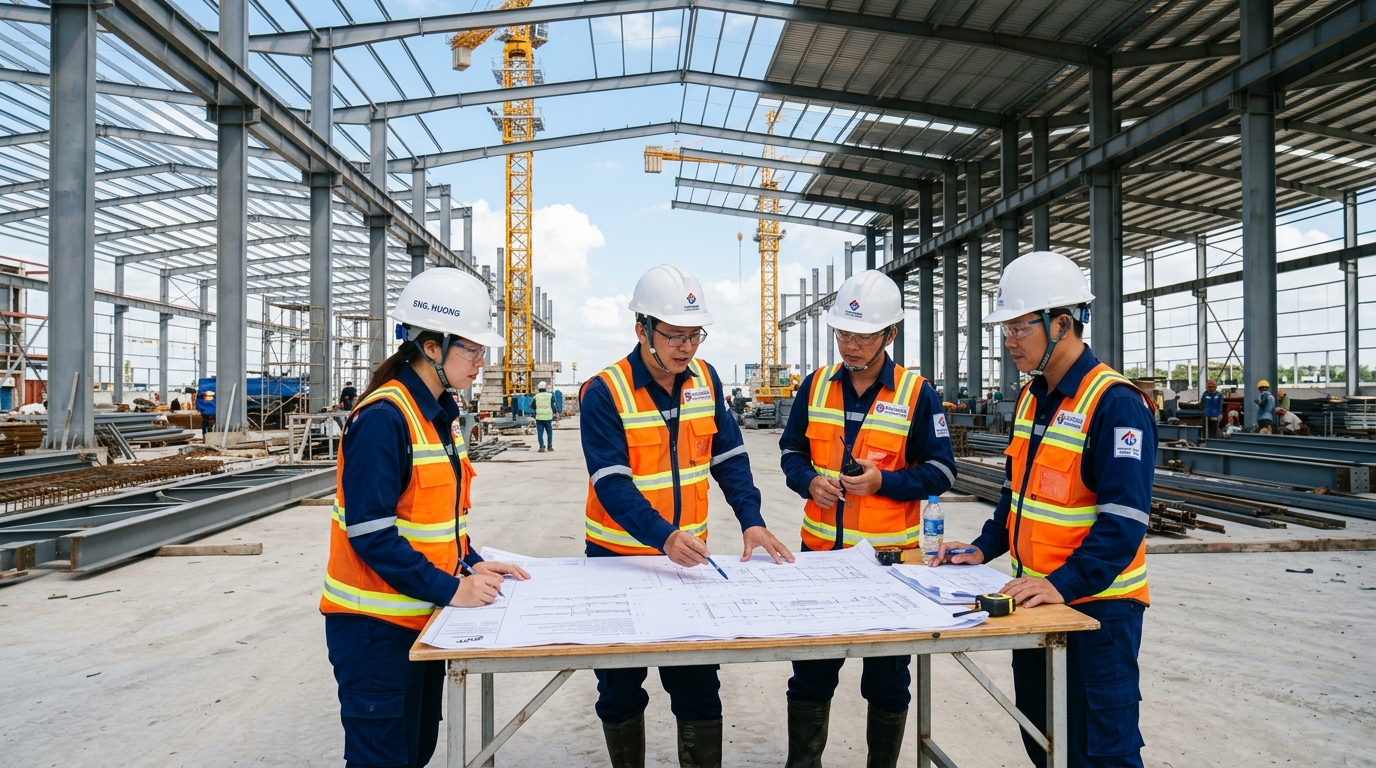
\includegraphics[width=186mm]{../../public/engineer-team-site.jpg}};
  \fill[TTCDeepNavy, opacity=0.82] (0,0) rectangle (68,72);
  \fill[TTCDeepNavy, opacity=0.38] (68,0) rectangle (92,72);

  \node[anchor=west, text width=54mm, align=left, text=white] at (8,48) {
    {\fontsize{7}{8}\selectfont\bfseries\color{TTCCyan} PEOPLE AT THE POINT OF EXECUTION}\\[1.5mm]
    {\fontsize{16}{18}\selectfont\bfseries CON NGƯỜI TẠI\\ĐIỂM THỰC THI}\\[2mm]
    {\fontsize{7.2}{9}\selectfont\color{white!84!gray}
    Đội ngũ dự án được tổ chức theo nhiệm vụ, có quyền hạn rõ ràng và một tuyến báo cáo duy nhất.}
  };

  \node[
    anchor=south east, rounded corners=3pt,
    fill=white, fill opacity=0.93, text opacity=1,
    draw=TTCCyan, line width=0.7pt,
    minimum width=52mm, minimum height=14mm, align=center
  ] at (179,7) {
    {\fontsize{8}{9.5}\selectfont\bfseries\color{TTCBlue} FIELD-LED DECISION MAKING}\\[0.7mm]
    {\fontsize{6.5}{8}\selectfont\color{TTCTextDark}Quyết định kỹ thuật được đưa đến gần hiện trường}
  };
  \draw[white, line width=1pt, rounded corners=3pt] (0.6,0.6) rectangle (185.4,71.4);
  \draw[TTCBorder, line width=0.65pt, rounded corners=3pt] (0,0) rectangle (186,72);
\end{tikzpicture}

\vspace{3mm}

% ACCOUNTABLE ROLES BY PROJECT PHASE
\noindent
\begin{tikzpicture}[x=1mm,y=1mm]
  \path[use as bounding box] (0,0) rectangle (186,67);
  \node[anchor=west, align=left] at (0,62) {
    {\fontsize{7}{8}\selectfont\bfseries\color{TTCCyan} PROJECT TEAM BY PHASE}\quad
    {\fontsize{9.5}{11}\selectfont\bfseries\color{TTCBlue} VAI TRÒ CHỊU TRÁCH NHIỆM THEO GIAI ĐOẠN}
  };

  % Phase 01
  \fill[white, rounded corners=3pt] (0,0) rectangle (58,55);
  \draw[TTCBorder, line width=0.65pt, rounded corners=3pt] (0,0) rectangle (58,55);
  \fill[TTCLightBlue, rounded corners=3pt] (0,43) rectangle (58,55);
  \node[anchor=west] at (5,49) {
    {\fontsize{7}{8}\selectfont\bfseries\color{TTCCyan} 01 / PRE-CONSTRUCTION}
  };
  \node[anchor=north west, text width=48mm, align=left] at (5,39) {
    {\fontsize{9.5}{11}\selectfont\bfseries\color{TTCBlue} CHUẨN BỊ \& THIẾT KẾ}\\[1.2mm]
    {\fontsize{7}{8.6}\selectfont\color{TTCTextDark}
    \textbf{Project Director}\\
    Đầu mối duy nhất với Chủ đầu tư.\\[0.8mm]
    \textbf{Design \& BIM Lead}\\
    Điều phối thiết kế, VE và mô hình.\\[0.8mm]
    \textbf{Planning / QS / FIDIC}\\
    Khóa phạm vi, tiến độ và ngân sách.}
  };
  \node[anchor=south, align=center] at (29,3.5) {
    {\fontsize{6.5}{7.8}\selectfont\bfseries\color{TTCRed} OUTPUT: APPROVED BASELINE}
  };

  % Phase 02
  \fill[white, rounded corners=3pt] (64,0) rectangle (122,55);
  \draw[TTCBlue!55!white, line width=0.75pt, rounded corners=3pt] (64,0) rectangle (122,55);
  \fill[TTCBlue, rounded corners=3pt] (64,43) rectangle (122,55);
  \node[anchor=west] at (69,49) {
    {\fontsize{7}{8}\selectfont\bfseries\color{white} 02 / CONSTRUCTION}
  };
  \node[anchor=north west, text width=48mm, align=left] at (69,39) {
    {\fontsize{9.5}{11}\selectfont\bfseries\color{TTCBlue} THI CÔNG HIỆN TRƯỜNG}\\[1.2mm]
    {\fontsize{7}{8.6}\selectfont\color{TTCTextDark}
    \textbf{Construction / Site Manager}\\
    Nguồn lực • mặt bằng • mũi thi công.\\[0.5mm]
    \textbf{Discipline Engineers}\\
    Kết cấu • Hạ tầng • MEP • PCCC.\\[0.5mm]
    \textbf{HSE \& QA/QC Managers}\\
    Quyền kiểm soát độc lập.}
  };
  \node[anchor=south, align=center] at (93,2.5) {
    {\fontsize{6.5}{7.8}\selectfont\bfseries\color{TTCRed} OUTPUT: CONTROLLED EXECUTION}
  };

  % Phase 03
  \fill[white, rounded corners=3pt] (128,0) rectangle (186,55);
  \draw[TTCBorder, line width=0.65pt, rounded corners=3pt] (128,0) rectangle (186,55);
  \fill[TTCLightBlue, rounded corners=3pt] (128,43) rectangle (186,55);
  \node[anchor=west] at (133,49) {
    {\fontsize{7}{8}\selectfont\bfseries\color{TTCCyan} 03 / HANDOVER \& O\&M}
  };
  \node[anchor=north west, text width=48mm, align=left] at (133,39) {
    {\fontsize{9.5}{11}\selectfont\bfseries\color{TTCBlue} BÀN GIAO \& VẬN HÀNH}\\[1.2mm]
    {\fontsize{7}{8.6}\selectfont\color{TTCTextDark}
    \textbf{Commissioning Manager}\\
    Điều phối thử nghiệm liên động.\\[0.8mm]
    \textbf{As-built \& Digital Twin Team}\\
    Chuẩn hóa hồ sơ và dữ liệu tài sản.\\[0.8mm]
    \textbf{Warranty Response Team}\\
    Tiếp nhận và xử lý kỹ thuật 24/7.}
  };
  \node[anchor=south, align=center] at (157,3.5) {
    {\fontsize{6.5}{7.8}\selectfont\bfseries\color{TTCRed} OUTPUT: READY FOR OPERATION}
  };
\end{tikzpicture}

\vspace{3mm}

% MOBILIZATION CHAIN — CLARIFIES HIERARCHY WITHOUT PORTRAIT PLACEHOLDERS
\noindent
\begin{tikzpicture}[x=1mm,y=1mm]
  \path[use as bounding box] (0,0) rectangle (186,29);
  \fill[TTCLightBlue, rounded corners=4pt] (0,0) rectangle (186,29);
  \draw[TTCBorder, line width=0.65pt, rounded corners=4pt] (0,0) rectangle (186,29);

  \node[align=center] at (22,14.5) {
    {\fontsize{6.5}{7.8}\selectfont\bfseries\color{TTCTextMuted} GOVERNANCE}\\[0.7mm]
    {\fontsize{9.2}{10.5}\selectfont\bfseries\color{TTCBlue} PMO TRỤ SỞ}\\[0.5mm]
    {\fontsize{6.4}{7.6}\selectfont Portfolio control}
  };
  \node[text=TTCRed] at (45,14.5) {\faChevronRight};
  \node[align=center] at (68,14.5) {
    {\fontsize{6.5}{7.8}\selectfont\bfseries\color{TTCTextMuted} ACCOUNTABILITY}\\[0.7mm]
    {\fontsize{9.2}{10.5}\selectfont\bfseries\color{TTCBlue} PROJECT DIRECTOR}\\[0.5mm]
    {\fontsize{6.4}{7.6}\selectfont Single point}
  };
  \node[text=TTCRed] at (93,14.5) {\faChevronRight};
  \node[align=center] at (118,14.5) {
    {\fontsize{6.5}{7.8}\selectfont\bfseries\color{TTCTextMuted} SITE AUTHORITY}\\[0.7mm]
    {\fontsize{9.2}{10.5}\selectfont\bfseries\color{TTCBlue} BAN CHỈ HUY}\\[0.5mm]
    {\fontsize{6.4}{7.6}\selectfont Daily execution}
  };
  \node[text=TTCRed] at (141,14.5) {\faChevronRight};
  \node[align=center] at (164,14.5) {
    {\fontsize{6.5}{7.8}\selectfont\bfseries\color{TTCTextMuted} DELIVERY}\\[0.7mm]
    {\fontsize{9.2}{10.5}\selectfont\bfseries\color{TTCRed} ĐỘI CHUYÊN MÔN}\\[0.5mm]
    {\fontsize{6.4}{7.6}\selectfont Task-based crews}
  };
\end{tikzpicture}

\vspace{3mm}

% CAPACITY SNAPSHOT
\noindent
\begin{tikzpicture}[x=1mm,y=1mm]
  \path[use as bounding box] (0,0) rectangle (186,27);
  \fill[white, rounded corners=4pt] (0,0) rectangle (186,27);
  \draw[TTCBorder, line width=0.65pt, rounded corners=4pt] (0,0) rectangle (186,27);
  \foreach \x in {46.5,93,139.5}{
    \draw[TTCBorder, line width=0.5pt] (\x,5) -- (\x,22);
  }
  \node[align=center] at (23.25,13.5) {
    {\fontsize{14}{15.5}\selectfont\bfseries\color{TTCRed} 350+}\\[0.8mm]
    {\fontsize{6.8}{8}\selectfont\bfseries\color{TTCTextDark} QUẢN LÝ \& KỸ SƯ}
  };
  \node[align=center] at (69.75,13.5) {
    {\fontsize{14}{15.5}\selectfont\bfseries\color{TTCBlue} 2.500+}\\[0.8mm]
    {\fontsize{6.8}{8}\selectfont\bfseries\color{TTCTextDark} CÔNG NHÂN KỸ THUẬT}
  };
  \node[align=center] at (116.25,13.5) {
    {\fontsize{14}{15.5}\selectfont\bfseries\color{TTCCyan} 85+}\\[0.8mm]
    {\fontsize{6.8}{8}\selectfont\bfseries\color{TTCTextDark} CHỈ HUY \& GIÁM SÁT}
  };
  \node[align=center] at (162.75,13.5) {
    {\fontsize{14}{15.5}\selectfont\bfseries\color{TTCBlue} 60+}\\[0.8mm]
    {\fontsize{6.8}{8}\selectfont\bfseries\color{TTCTextDark} KỸ SƯ BIM \& SỐ HÓA}
  };
\end{tikzpicture}
\end{minipage}
\newpage

% ============================================================
% TRANG 08: QUẢN TRỊ TÀI CHÍNH DỰ ÁN & KỶ LUẬT DÒNG TIỀN
% ============================================================
\pageheaderbar{QUẢN TRỊ TÀI CHÍNH DỰ ÁN \& KỶ LUẬT DÒNG TIỀN}{Trang 08}
\pagefooterbar{Trang 08}

\begin{tikzpicture}[remember picture, overlay]
  \node[opacity=0.025, scale=2.6, font=\bfseries\sffamily, text=TTCBlue]
    at ([yshift=-12mm]current page.center) {FINANCIAL GOVERNANCE \& DISCIPLINE};
  \draw[TTCBlue!6!white, line width=0.45pt]
    ([xshift=15mm, yshift=20mm]current page.south west)
    grid[step=8mm]
    ([xshift=195mm, yshift=45mm]current page.south west);
\end{tikzpicture}

\begin{minipage}[t][246mm]{\textwidth}
\secbrand{Quản Trị Tài Chính Dự Án \& Kỷ Luật Dòng Tiền}{Project Financial Governance • Cost Discipline • Verified \& Traceable Records}

\vspace{1mm}
{\fontsize{14.5}{16.5}\selectfont\bfseries\color{TTCBlue}
KIỂM SOÁT TỪ QUYẾT ĐỊNH NHẬN THẦU ĐẾN QUYẾT TOÁN CÔNG TRÌNH\par}
\vspace{1mm}
{\fontsize{7.5}{9}\selectfont\color{TTCTextMuted}
Mỗi dự án được thiết lập ngân sách độc lập, kiểm soát 4 cổng và đối chiếu định kỳ trước khi huy động nguồn lực.\par}
\vspace{3.5mm}

% ============================================================
% TẦNG 1: BỐN CỔNG KIỂM SOÁT TÀI CHÍNH + NGUYÊN TẮC QUẢN TRỊ
% ============================================================
\noindent
\begin{tikzpicture}[x=1mm,y=1mm]
  \path[use as bounding box] (0,0) rectangle (186,86);

  % KHỐI TRÁI: 4 CỔNG KIỂM SOÁT (126mm x 86mm)
  \fill[white, rounded corners=4pt] (0,0) rectangle (126,86);
  \draw[TTCBorder, line width=0.7pt, rounded corners=4pt] (0,0) rectangle (126,86);

  \node[anchor=west, text=TTCCyan, font=\fontsize{7}{8}\selectfont\bfseries]
    at (6,79.5) {FOUR FINANCIAL CONTROL GATES};
  \node[anchor=west, text=TTCBlue, font=\fontsize{10}{12}\selectfont\bfseries]
    at (6,72.5) {BỐN CỔNG KIỂM SOÁT TÀI CHÍNH DỰ ÁN};

  % Timeline connector bar
  \draw[TTCBlue!30!white, line width=1pt] (15,50) -- (111,50);

  % 4 Cổng Nodes & Contents
  % Cổng 01
  \fill[TTCRed] (15,50) circle (4.8);
  \node[text=white, font=\fontsize{7}{8}\selectfont\bfseries] at (15,50) {01};
  \node[anchor=south, align=center, text width=26mm, text=TTCRed, font=\fontsize{7}{8.2}\selectfont\bfseries]
    at (15,57.5) {THẨM ĐỊNH\\HỢP ĐỒNG};
  \node[anchor=north, align=center, text width=27mm, text=TTCTextDark, font=\fontsize{6.2}{7.6}\selectfont]
    at (15,42.5) {Biên lợi nhuận\\Điều khoản thanh toán\\Rủi ro giữ lại};

  % Cổng 02
  \fill[white] (47,50) circle (4.8);
  \draw[TTCBlue, line width=0.85pt] (47,50) circle (4.8);
  \node[text=TTCBlue, font=\fontsize{7}{8}\selectfont\bfseries] at (47,50) {02};
  \node[anchor=south, align=center, text width=26mm, text=TTCBlue, font=\fontsize{7}{8.2}\selectfont\bfseries]
    at (47,57.5) {NGÂN SÁCH\\DỰ ÁN};
  \node[anchor=north, align=center, text width=27mm, text=TTCTextDark, font=\fontsize{6.2}{7.6}\selectfont]
    at (47,42.5) {Chi phí cơ sở (Baseline)\\Kế hoạch dòng tiền\\Hạn mức giải ngân};

  % Cổng 03
  \fill[white] (79,50) circle (4.8);
  \draw[TTCBlue, line width=0.85pt] (79,50) circle (4.8);
  \node[text=TTCBlue, font=\fontsize{7}{8}\selectfont\bfseries] at (79,50) {03};
  \node[anchor=south, align=center, text width=26mm, text=TTCBlue, font=\fontsize{7}{8.2}\selectfont\bfseries]
    at (79,57.5) {KIỂM SOÁT\\THỰC HIỆN};
  \node[anchor=north, align=center, text width=27mm, text=TTCTextDark, font=\fontsize{6.2}{7.6}\selectfont]
    at (79,42.5) {So sánh Kế hoạch - Thực tế\\Duyệt phát sinh (VO)\\Dự báo hoàn thành (EAC)};

  % Cổng 04
  \fill[white] (111,50) circle (4.8);
  \draw[TTCBlue, line width=0.85pt] (111,50) circle (4.8);
  \node[text=TTCBlue, font=\fontsize{7}{8}\selectfont\bfseries] at (111,50) {04};
  \node[anchor=south, align=center, text width=26mm, text=TTCBlue, font=\fontsize{7}{8.2}\selectfont\bfseries]
    at (111,57.5) {NGHIỆM THU\\QUYẾT TOÁN};
  \node[anchor=north, align=center, text width=27mm, text=TTCTextDark, font=\fontsize{6.2}{7.6}\selectfont]
    at (111,42.5) {Hồ sơ khối lượng hoàn công\\Thu hồi công nợ\\Đóng mã chi phí dự án};

  % Dải cam kết phía dưới khối trái
  \fill[TTCDeepNavy, rounded corners=3pt] (5,5.5) rectangle (121,18.5);
  \node[anchor=west, text=TTCCyan, font=\fontsize{6.8}{8}\selectfont\bfseries]
    at (8,12) {\faShield*\quad CONTROL BEFORE COMMITMENT};
  \node[anchor=east, text=white, font=\fontsize{6.5}{7.8}\selectfont\bfseries]
    at (118,12) {Chỉ cam kết khi ngân sách \& dòng tiền đã phê duyệt};

  % KHỐI PHẢI: NGUYÊN TẮC QUẢN TRỊ (55mm x 86mm)
  \fill[TTCLightBlue, rounded corners=4pt] (131,0) rectangle (186,86);
  \draw[TTCBorder, line width=0.7pt, rounded corners=4pt] (131,0) rectangle (186,86);

  \node[anchor=north west, text=TTCCyan, font=\fontsize{7}{8}\selectfont\bfseries]
    at (136,79.5) {CONTROL PRINCIPLE};
  \node[anchor=north west, text width=46mm, text=TTCBlue, font=\fontsize{9.5}{11.5}\selectfont\bfseries]
    at (136,73) {KHÔNG NHẬN THẦU VƯỢT NĂNG LỰC};
  \fill[TTCRed] (136,61.5) rectangle (152,63);

  \node[anchor=north west, text width=45mm, text=TTCTextDark, font=\fontsize{6.8}{8.6}\selectfont]
    at (136,56) {
    \textcolor{TTCRed}{\faCheckCircle}\ \textbf{Khóa ngân sách:} Duyệt 100\% trước khi huy động nguồn lực.\\[2.4mm]
    \textcolor{TTCRed}{\faCheckCircle}\ \textbf{Kiểm soát phát sinh:} Mọi chi phí ngoài HĐ phải có nguồn bù.\\[2.4mm]
    \textcolor{TTCRed}{\faCheckCircle}\ \textbf{Tăng trưởng an toàn:} Quy mô chỉ mở rộng khi bàn giao sẵn sàng.
  };

  \fill[white, rounded corners=2.5pt, draw=TTCBorder, line width=0.55pt] (136,6) rectangle (181,18);
  \node[anchor=center, text=TTCBlue, font=\fontsize{6.6}{8}\selectfont\bfseries, align=center]
    at (158.5,12) {\faLock\quad 100\% DỰ ÁN CÓ MÃ CHI PHÍ RIÊNG};
\end{tikzpicture}

\vspace{3.5mm}

% ============================================================
% TẦNG 2: BA TRỤ CỘT QUẢN TRỊ TÀI CHÍNH
% ============================================================
\noindent
\begin{tikzpicture}[x=1mm,y=1mm]
  \path[use as bounding box] (0,0) rectangle (186,58);

  % 3 Cột: Kiểm soát chi phí | Kiểm soát công nợ | Hồ sơ truy xuất (58mm mỗi cột)
  % Card 1: Cost Control
  \fill[white, rounded corners=4pt] (0,0) rectangle (58,58);
  \draw[TTCBorder, line width=0.65pt, rounded corners=4pt] (0,0) rectangle (58,58);
  \fill[TTCRed, rounded corners=1pt] (5,50.5) rectangle (22,52.5);
  \node[anchor=north west, text width=50mm, align=left] at (5,47.5) {
    {\fontsize{7}{8.2}\selectfont\bfseries\color{TTCRed}\faCalculator\quad COST CONTROL}\\[1.2mm]
    {\fontsize{9.8}{11.5}\selectfont\bfseries\color{TTCBlue} KIỂM SOÁT CHI PHÍ}\\[2mm]
    {\fontsize{6.6}{8.2}\selectfont\color{TTCTextDark}
    \textbullet\ Thiết lập ngân sách cơ sở (Baseline) theo WBS.\newline
    \textbullet\ Báo cáo phương sai chi phí hàng tuần.\newline
    \textbullet\ Dự báo tổng chi phí hoàn thành (EAC).}
  };

  % Card 2: Receivable Control
  \fill[white, rounded corners=4pt] (64,0) rectangle (122,58);
  \draw[TTCBorder, line width=0.65pt, rounded corners=4pt] (64,0) rectangle (122,58);
  \fill[TTCCyan, rounded corners=1pt] (69,50.5) rectangle (86,52.5);
  \node[anchor=north west, text width=50mm, align=left] at (69,47.5) {
    {\fontsize{7}{8.2}\selectfont\bfseries\color{TTCCyan}\faFileInvoiceDollar\quad RECEIVABLE CONTROL}\\[1.2mm]
    {\fontsize{9.8}{11.5}\selectfont\bfseries\color{TTCBlue} KIỂM SOÁT CÔNG NỢ}\\[2mm]
    {\fontsize{6.6}{8.2}\selectfont\color{TTCTextDark}
    \textbullet\ Bám sát mốc nghiệm thu khối lượng ITP.\newline
    \textbullet\ Theo dõi dòng tiền thanh toán \& tạm ứng.\newline
    \textbullet\ Quản trị chặt chẽ khoản giữ lại bảo hành.}
  };

  % Card 3: Verified Reporting
  \fill[white, rounded corners=4pt] (128,0) rectangle (186,58);
  \draw[TTCBorder, line width=0.65pt, rounded corners=4pt] (128,0) rectangle (186,58);
  \fill[TTCBlue, rounded corners=1pt] (133,50.5) rectangle (150,52.5);
  \node[anchor=north west, text width=50mm, align=left] at (133,47.5) {
    {\fontsize{7}{8.2}\selectfont\bfseries\color{TTCBlue}\faClipboardCheck\quad VERIFIED REPORTING}\\[1.2mm]
    {\fontsize{9.8}{11.5}\selectfont\bfseries\color{TTCBlue} HỒ SƠ TRUY XUẤT}\\[2mm]
    {\fontsize{6.6}{8.2}\selectfont\color{TTCTextDark}
    \textbullet\ Dữ liệu chi phí đồng bộ thời gian thực.\newline
    \textbullet\ Báo cáo quản trị đa kỳ theo chuẩn quốc tế.\newline
    \textbullet\ Sẵn sàng kiểm toán độc lập theo yêu cầu CĐT.}
  };
\end{tikzpicture}

\vspace{3.5mm}

% ============================================================
% TẦNG 3: GÓI HỒ SƠ MINH CHỨNG & CHÍNH SÁCH BẢO MẬT
% ============================================================
\noindent
\begin{tikzpicture}[x=1mm,y=1mm]
  \path[use as bounding box] (0,0) rectangle (186,46);

  % Outer Card
  \fill[white, rounded corners=4pt] (0,0) rectangle (186,46);
  \draw[TTCBorder, line width=0.65pt, rounded corners=4pt] (0,0) rectangle (186,46);

  % Left Navy Brand Anchor (48mm x 46mm)
  \fill[TTCDeepNavy, rounded corners=4pt] (0,0) rectangle (48,46);
  \node[anchor=west, text width=40mm, align=left] at (6,23) {
    {\fontsize{7}{8}\selectfont\bfseries\color{TTCCyan} DISCLOSURE POLICY}\\[1.2mm]
    {\fontsize{9}{11}\selectfont\bfseries\color{white} MINH BẠCH CÓ\\KIỂM SOÁT}\\[1.8mm]
    {\fontsize{6}{7.2}\selectfont\color{white!75!gray}Verified data \textbullet\ Right audience}
  };

  % 4 Pill Cards on the Right
  \foreach \xa/\xb/\num/\label/\sub in {
    53/81/01/BÁO CÁO TÀI CHÍNH/Kiểm toán độc lập,
    85/113/02/HỒ SƠ THUẾ/Nghĩa vụ Nhà nước,
    117/145/03/ĐỐI CHIẾU CÔNG NỢ/0 nợ đọng NCC,
    149/181/04/BÁO CÁO QUẢN TRỊ/Dòng tiền dự án}{
    \fill[TTCLightBlue, rounded corners=3pt] (\xa,14) rectangle (\xb,40);
    \draw[TTCBorder, line width=0.5pt, rounded corners=3pt] (\xa,14) rectangle (\xb,40);
    \node[text=TTCRed, font=\fontsize{8}{9.5}\selectfont\bfseries] at ({(\xa+\xb)/2},34.5) {\num};
    \node[align=center, text width=26mm, text=TTCBlue, font=\fontsize{6.5}{7.8}\selectfont\bfseries]
      at ({(\xa+\xb)/2},26) {\label};
    \node[align=center, text width=26mm, text=TTCTextMuted, font=\fontsize{5.8}{7}\selectfont]
      at ({(\xa+\xb)/2},18.5) {\sub};
  }

  % Bottom Security Notice
  \draw[TTCBorder, line width=0.5pt] (53,9.5) -- (181,9.5);
  \node[anchor=south west, text=TTCTextMuted, font=\fontsize{6}{7.3}\selectfont\itshape]
    at (53,3) {\faLock\quad Số liệu chi tiết được cung cấp theo hồ sơ mời thầu hoặc thỏa thuận bảo mật NDA với Chủ đầu tư.};
\end{tikzpicture}
\end{minipage}
\newpage

% ============================================================
% TRANG 09: NĂNG LỰC HUY ĐỘNG CHO DỰ ÁN EPC
% ============================================================
\pageheaderbar{HẠN MỨC TÍN DỤNG \& NGUỒN LỰC TRIỂN KHAI}{Trang 09}
\pagefooterbar{Trang 09}

\begin{tikzpicture}[remember picture, overlay]
  \node[opacity=0.02, scale=2.4, font=\bfseries\sffamily, text=TTCBlue]
    at ([yshift=-12mm]current page.center) {BANKING CAPACITY \& SITE MOBILIZATION};
  \draw[TTCBlue!6!white, line width=0.45pt]
    ([xshift=15mm, yshift=20mm]current page.south west)
    grid[step=8mm]
    ([xshift=195mm, yshift=45mm]current page.south west);
\end{tikzpicture}

\begin{minipage}[t][246mm]{\textwidth}
\secbrand{Năng Lực Huy Động Cho Dự Án EPC}{Banking Capacity, Performance Bonds \& Site-Ready Workforce Mobilization}

\vspace{1mm}
{\fontsize{14.5}{16.5}\selectfont\bfseries\color{TTCBlue}
HAI NGUỒN LỰC • MỘT KẾ HOẠCH HUY ĐỘNG TOÀN DIỆN\par}
\vspace{1mm}
{\fontsize{7.5}{9}\selectfont\color{TTCTextMuted}
Công cụ tài chính vững chắc kết hợp lực lượng thi công tinh nhuệ, sẵn sàng kích hoạt theo từng mốc hợp đồng.\par}
\vspace{3.5mm}

% ============================================================
% TẦNG 1: HAI ĐỘNG CƠ HUY ĐỘNG (FINANCIAL ENGINE & DELIVERY ENGINE)
% ============================================================
\noindent
\begin{tikzpicture}[x=1mm,y=1mm]
  \path[use as bounding box] (0,0) rectangle (186,80);

  % KHỐI TRÁI: FINANCIAL ENGINE (HẠN MỨC TÍN DỤNG 250 TỶ)
  \fill[white, rounded corners=4pt] (0,0) rectangle (90,80);
  \draw[TTCBorder, line width=0.7pt, rounded corners=4pt] (0,0) rectangle (90,80);

  \node[anchor=north west, text=TTCCyan, font=\fontsize{7}{8}\selectfont\bfseries]
    at (6,73.5) {FINANCIAL ENGINE};
  \node[anchor=north west, text=TTCBlue, font=\fontsize{10}{12}\selectfont\bfseries]
    at (6,67) {NĂNG LỰC TÍN DỤNG \& BẢO LÃNH};

  \node[anchor=west] at (6,54) {
    {\fontsize{25}{27}\selectfont\bfseries\color{TTCRed} 250 TỶ}\quad
    {\fontsize{7.5}{9}\selectfont\bfseries\color{TTCTextMuted} HẠN MỨC TÍN DỤNG}
  };

  % Bank Badges
  \fill[TTCLightBlue, rounded corners=2.5pt, draw=TTCBorder, line width=0.5pt] (5,38) rectangle (85,46);
  \node[anchor=center, text=TTCBlue, font=\fontsize{6.2}{7.4}\selectfont\bfseries]
    at (45,42) {Vietcombank \textbullet\ BIDV \textbullet\ VietinBank \textbullet\ TPBank \textbullet\ ACB \textbullet\ MB};

  \node[anchor=north west, text width=80mm, text=TTCTextDark, font=\fontsize{6.8}{8.6}\selectfont]
    at (6,33.5) {
    \textcolor{TTCRed}{\faCheckCircle}\ \textbf{Bảo lãnh hợp đồng:} Dự thầu, thực hiện, tạm ứng \& bảo hành.\\[1.4mm]
    \textcolor{TTCRed}{\faCheckCircle}\ \textbf{Tốc độ phát hành:} Cấp thư bảo lãnh ngân hàng trong 24--48h.\\[1.4mm]
    \textcolor{TTCRed}{\faCheckCircle}\ \textbf{Chuẩn quốc tế:} Tuân thủ điều ước FIDIC Silver Book \& Mở L/C thép.
  };

  % KHỐI PHẢI: DELIVERY ENGINE (NGUỒN LỰC 2.850+ NHÂN SỰ)
  \fill[white, rounded corners=4pt] (96,0) rectangle (186,80);
  \draw[TTCBorder, line width=0.7pt, rounded corners=4pt] (96,0) rectangle (186,80);

  \node[anchor=north west, text=TTCCyan, font=\fontsize{7}{8}\selectfont\bfseries]
    at (102,73.5) {DELIVERY ENGINE};
  \node[anchor=north west, text=TTCBlue, font=\fontsize{10}{12}\selectfont\bfseries]
    at (102,67) {LỰC LƯỢNG TRIỂN KHAI THỰC CHIẾN};

  \node[anchor=west] at (102,54) {
    {\fontsize{25}{27}\selectfont\bfseries\color{TTCBlue} 2.850+}\quad
    {\fontsize{7.5}{9}\selectfont\bfseries\color{TTCTextMuted} NHÂN SỰ ĐA CHUYÊN NGÀNH}
  };

  % Visual Distribution Bar
  \fill[TTCBlue, rounded corners=1.5pt] (102,41) rectangle (114,45);
  \fill[TTCCyan, rounded corners=1.5pt] (115,41) rectangle (180,45);
  \node[anchor=west, text=TTCBlue, font=\fontsize{6.2}{7.4}\selectfont\bfseries] at (102,47.5) {350+ Kỹ sư (12\%)};
  \node[anchor=east, text=TTCCyan, font=\fontsize{6.6}{7.6}\selectfont\bfseries] at (180,47.5) {2.500+ Công nhân xây lắp (88\%)};

  \node[anchor=north west, text width=78mm, text=TTCTextDark, font=\fontsize{6.8}{8.6}\selectfont]
    at (102,33.5) {
    \textcolor{TTCBlue}{\faCheckCircle}\ \textbf{350+ Quản lý \& Kỹ sư:} CCHN Hạng II, BIM/Tekla LOD 400, QA/QC \& HSE.\\[1.4mm]
    \textcolor{TTCCyan}{\faCheckCircle}\ \textbf{2.500+ Thợ lành nghề:} Hàn AWS D1.1 (3G-6G), Lắp dựng PEB, MEP/PCCC.\\[1.4mm]
    \textcolor{TTCTextMuted}{\faCheckCircle}\ \textbf{Tổ chức thi công:} 3 ca liên tục, sẵn sàng điều động đồng thời 5--8 dự án.
  };

  % Joining Connector Pill
  \fill[white] (93,54) circle (4);
  \draw[TTCCyan, line width=0.8pt] (93,54) circle (4);
  \node[text=TTCRed, font=\fontsize{10}{11}\selectfont\bfseries] at (93,54) {+};
\end{tikzpicture}

\vspace{3.5mm}

% ============================================================
% TẦNG 2: 4 GIAI ĐOẠN KÍCH HOẠT HỢP ĐỒNG (CONTRACT LIFECYCLE)
% ============================================================
\noindent
\begin{tikzpicture}[x=1mm,y=1mm]
  \path[use as bounding box] (0,0) rectangle (186,84);

  \node[anchor=west] at (0,79) {
    {\fontsize{7}{8}\selectfont\bfseries\color{TTCCyan} CONTRACT LIFECYCLE}\quad
    {\fontsize{9.8}{11.5}\selectfont\bfseries\color{TTCBlue} NGUỒN LỰC ĐƯỢC KÍCH HOẠT THEO TỪNG GIAI ĐOẠN}
  };

  % 4 Stages: 01 Tender | 02 Award | 03 Delivery | 04 Handover (42.5mm mỗi card)
  % Stage 01: Tender
  \fill[white, rounded corners=3.5pt] (0,0) rectangle (42,72);
  \draw[TTCBorder, line width=0.65pt, rounded corners=3.5pt] (0,0) rectangle (42,72);
  \fill[TTCLightBlue, rounded corners=3.5pt] (0,59) rectangle (42,72);
  \node[anchor=west] at (4,65.5) {
    {\fontsize{7}{8}\selectfont\bfseries\color{TTCCyan} 01 / TENDER}
  };
  \node[anchor=north west, text width=34mm, align=left] at (4,53) {
    {\fontsize{9.8}{11.5}\selectfont\bfseries\color{TTCBlue} DỰ THẦU}\\[2.2mm]
    {\fontsize{6.5}{7.8}\selectfont\bfseries\color{TTCTextMuted} TÀI CHÍNH}\\[0.7mm]
    {\fontsize{6.8}{8.2}\selectfont\color{TTCTextDark}Bảo lãnh dự thầu 1--3\% \& hạn mức tín dụng.}\\[2mm]
    {\fontsize{6.5}{7.8}\selectfont\bfseries\color{TTCTextMuted} NHÂN LỰC}\\[0.7mm]
    {\fontsize{6.8}{8.2}\selectfont\color{TTCTextDark}Đấu thầu, QS, Kỹ thuật VE \& hợp đồng FIDIC.}
  };
  \fill[TTCLightBlue, rounded corners=2pt, draw=TTCBorder, line width=0.5pt] (6,3.5) rectangle (36,10);
  \node[anchor=center] at (21,6.75) {
    {\fontsize{6.4}{7.8}\selectfont\bfseries\color{TTCBlue} BID-READY}
  };

  % Chevron 1 -> 2
  \node[text=TTCRed] at (45,36) {\faChevronRight};

  % Stage 02: Award
  \fill[white, rounded corners=3.5pt] (48,0) rectangle (90,72);
  \draw[TTCBorder, line width=0.65pt, rounded corners=3.5pt] (48,0) rectangle (90,72);
  \fill[TTCLightBlue, rounded corners=3.5pt] (48,59) rectangle (90,72);
  \node[anchor=west] at (52,65.5) {
    {\fontsize{7}{8}\selectfont\bfseries\color{TTCCyan} 02 / AWARD}
  };
  \node[anchor=north west, text width=34mm, align=left] at (52,53) {
    {\fontsize{9.8}{11.5}\selectfont\bfseries\color{TTCBlue} KÝ HỢP ĐỒNG}\\[2.2mm]
    {\fontsize{6.5}{7.8}\selectfont\bfseries\color{TTCTextMuted} TÀI CHÍNH}\\[0.7mm]
    {\fontsize{6.8}{8.2}\selectfont\color{TTCTextDark}Bảo lãnh thực hiện 5--10\% \& tạm ứng 10--20\%.}\\[2mm]
    {\fontsize{6.5}{7.8}\selectfont\bfseries\color{TTCTextMuted} NHÂN LỰC}\\[0.7mm]
    {\fontsize{6.8}{8.2}\selectfont\color{TTCTextDark}Bổ nhiệm Project Director, PMO \& Core Team.}
  };
  \fill[TTCLightBlue, rounded corners=2pt, draw=TTCBorder, line width=0.5pt] (54,3.5) rectangle (84,10);
  \node[anchor=center] at (69,6.75) {
    {\fontsize{6.4}{7.8}\selectfont\bfseries\color{TTCBlue} CONTRACT-READY}
  };

  % Chevron 2 -> 3
  \node[text=TTCRed] at (93,36) {\faChevronRight};

  % Stage 03: Delivery
  \fill[white, rounded corners=3.5pt] (96,0) rectangle (138,72);
  \draw[TTCBlue!60!white, line width=0.75pt, rounded corners=3.5pt] (96,0) rectangle (138,72);
  \fill[TTCBlue, rounded corners=3.5pt] (96,59) rectangle (138,72);
  \node[anchor=west] at (100,65.5) {
    {\fontsize{7}{8}\selectfont\bfseries\color{white} 03 / DELIVERY}
  };
  \node[anchor=north west, text width=34mm, align=left] at (100,53) {
    {\fontsize{9.8}{11.5}\selectfont\bfseries\color{TTCBlue} TRIỂN KHAI}\\[2.2mm]
    {\fontsize{6.5}{7.8}\selectfont\bfseries\color{TTCTextMuted} TÀI CHÍNH}\\[0.7mm]
    {\fontsize{6.8}{8.2}\selectfont\color{TTCTextDark}Vốn lưu động, L/C vật tư \& thanh toán NCC.}\\[2mm]
    {\fontsize{6.5}{7.8}\selectfont\bfseries\color{TTCTextMuted} NHÂN LỰC}\\[0.7mm]
    {\fontsize{6.8}{8.2}\selectfont\color{TTCTextDark}Ban chỉ huy, Kỹ sư hiện trường \& Đội thợ 3 ca.}
  };
  \fill[TTCBlue, rounded corners=2pt] (102,3.5) rectangle (132,10);
  \node[anchor=center] at (117,6.75) {
    {\fontsize{6.4}{7.8}\selectfont\bfseries\color{white} SITE-READY}
  };

  % Chevron 3 -> 4
  \node[text=TTCRed] at (141,36) {\faChevronRight};

  % Stage 04: Handover
  \fill[white, rounded corners=3.5pt] (144,0) rectangle (186,72);
  \draw[TTCRed!70!white, line width=0.75pt, rounded corners=3.5pt] (144,0) rectangle (186,72);
  \fill[TTCRed, rounded corners=3.5pt] (144,59) rectangle (186,72);
  \node[anchor=west] at (148,65.5) {
    {\fontsize{7}{8}\selectfont\bfseries\color{white} 04 / HANDOVER}
  };
  \node[anchor=north west, text width=34mm, align=left] at (148,53) {
    {\fontsize{9.8}{11.5}\selectfont\bfseries\color{TTCBlue} BÀN GIAO}\\[2.2mm]
    {\fontsize{6.5}{7.8}\selectfont\bfseries\color{TTCTextMuted} TÀI CHÍNH}\\[0.7mm]
    {\fontsize{6.8}{8.2}\selectfont\color{TTCTextDark}Bảo lãnh bảo hành 5\%, duy trì trọn 24 tháng.}\\[2mm]
    {\fontsize{6.5}{7.8}\selectfont\bfseries\color{TTCTextMuted} NHÂN LỰC}\\[0.7mm]
    {\fontsize{6.8}{8.2}\selectfont\color{TTCTextDark}Commissioning, As-Built \& Bảo hành 24/7.}
  };
  \fill[TTCRed, rounded corners=2pt] (150,3.5) rectangle (180,10);
  \node[anchor=center] at (165,6.75) {
    {\fontsize{6.4}{7.8}\selectfont\bfseries\color{white} O\&M-READY}
  };
\end{tikzpicture}

\vspace{3.5mm}

% ============================================================
% TẦNG 3: BĂNG CAM KẾT SẴN SÀNG HUY ĐỘNG (MOBILIZATION ASSURANCE)
% ============================================================
\noindent
\begin{tikzpicture}[x=1mm,y=1mm]
  \path[use as bounding box] (0,0) rectangle (186,43);

  % Outer Card
  \fill[white, rounded corners=4pt] (0,0) rectangle (186,43);
  \draw[TTCBorder, line width=0.65pt, rounded corners=4pt] (0,0) rectangle (186,43);

  % Left Navy Brand Anchor (48mm x 43mm)
  \fill[TTCDeepNavy, rounded corners=4pt] (0,0) rectangle (48,43);
  \node[anchor=west, text width=40mm, align=left] at (6,21.5) {
    {\fontsize{7}{8}\selectfont\bfseries\color{TTCCyan} ASSURANCE}\\[1mm]
    {\fontsize{8.8}{10.5}\selectfont\bfseries\color{white} ĐIỀU KIỆN\\SẴN SÀNG}\\[1.5mm]
    {\fontsize{6}{7.2}\selectfont\color{white!75!gray}Financial \textbullet\ Technical \textbullet\ HSE}
  };

  % 4 Metric Badges on Right
  \foreach \xa/\xb/\val/\title/\sub in {
    53/81/0/NỢ QUÁ HẠN/Bảo toàn dòng tiền,
    85/113/100\%/ĐÀO TẠO HSE/Thẻ an toàn Nhóm 3,
    117/145/AWS D1.1/THỢ HÀN 3G-6G/Sát hạch quốc tế,
    149/181/FDI READY/ĐA NGÔN NGỮ/Anh • Hàn • Trung}{
    \fill[TTCLightBlue, rounded corners=3pt] (\xa,4.5) rectangle (\xb,38.5);
    \draw[TTCBorder, line width=0.5pt, rounded corners=3pt] (\xa,4.5) rectangle (\xb,38.5);
    \node[text=TTCRed, font=\fontsize{11}{13}\selectfont\bfseries] at ({(\xa+\xb)/2},29.5) {\val};
    \node[align=center, text width=26mm, text=TTCBlue, font=\fontsize{6.4}{7.6}\selectfont\bfseries]
      at ({(\xa+\xb)/2},19.5) {\title};
    \node[align=center, text width=26mm, text=TTCTextMuted, font=\fontsize{5.8}{7}\selectfont]
      at ({(\xa+\xb)/2},11) {\sub};
  }
\end{tikzpicture}
\end{minipage}
\newpage

% ============================================================
% TRANG 10: TALENT DEVELOPMENT JOURNEY & SAFETY CULTURE
% ============================================================
\pageheaderbar{ĐÀO TẠO NĂNG LỰC \& VĂN HÓA AN TOÀN}{Trang 10}
\pagefooterbar{Trang 10}

\begin{tikzpicture}[remember picture, overlay]
  \node[opacity=0.02, scale=2.4, font=\bfseries\sffamily, text=TTCBlue]
    at ([yshift=-12mm]current page.center) {TALENT DEVELOPMENT \& SAFETY CULTURE};
  \draw[TTCBlue!6!white, line width=0.45pt]
    ([xshift=15mm, yshift=20mm]current page.south west)
    grid[step=8mm]
    ([xshift=195mm, yshift=45mm]current page.south west);
\end{tikzpicture}

\begin{minipage}[t][246mm]{\textwidth}
\secbrand{Hành Trình Phát Triển Năng Lực}{Talent Development, Technical Certification \& Safety-First Culture}

\vspace{1mm}
{\fontsize{14.5}{16.5}\selectfont\bfseries\color{TTCBlue}
HỌC ĐÚNG VIỆC • CHỨNG NHẬN ĐÚNG CHUẨN • DẪN DẮT DỰ ÁN\par}
\vspace{1mm}
{\fontsize{7.5}{9}\selectfont\color{TTCTextMuted}
Hệ thống đào tạo gắn liền thực chiến hiện trường, biến tri thức chuyên môn thành kết quả thi công an toàn.\par}
\vspace{3.5mm}

% ============================================================
% TRAINING HERO BANNER
% ============================================================
\noindent
\begin{tikzpicture}[x=1mm,y=1mm]
  \path[use as bounding box] (0,0) rectangle (186,65);
  \clip[rounded corners=3pt] (0,0) rectangle (186,65);
  \node[anchor=center, inner sep=0pt] at (93,32.5)
    {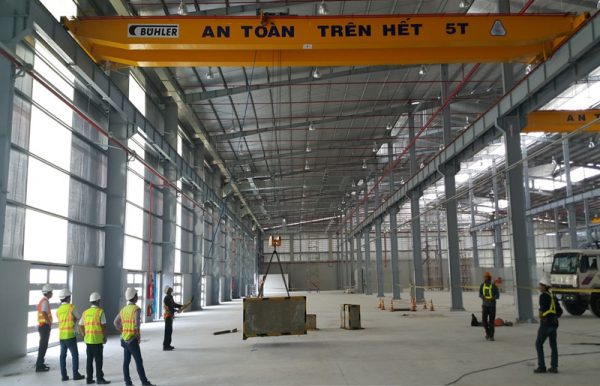
\includegraphics[width=186mm]{../../public/introsection1.jpg}};
  \fill[TTCDeepNavy, opacity=0.84] (0,0) rectangle (74,65);
  \fill[TTCDeepNavy, opacity=0.28] (74,0) rectangle (98,65);
  \node[anchor=west, text width=60mm, align=left, text=white] at (8,43) {
    {\fontsize{7}{8}\selectfont\bfseries\color{TTCCyan} FIELD-BASED LEARNING}\\[1.4mm]
    {\fontsize{15}{17}\selectfont\bfseries HỌC TẠI\\ĐIỂM THỰC THI}\\[1.8mm]
    {\fontsize{7}{8.6}\selectfont\color{white!82!gray}
    Đào tạo gắn với tình huống thật, thiết bị thật và quyền dừng công việc khi không an toàn.}
  };
  \node[
    anchor=south east, rounded corners=3pt,
    fill=white, fill opacity=0.94, text opacity=1,
    draw=TTCCyan, line width=0.65pt,
    minimum width=52mm, minimum height=13mm, align=center
  ] at (179,7) {
    {\fontsize{8.2}{9.5}\selectfont\bfseries\color{TTCBlue} SAFETY BEFORE PRODUCTIVITY}\\[0.6mm]
    {\fontsize{6.4}{7.8}\selectfont\color{TTCTextDark}An toàn là điều kiện tiên quyết để bắt đầu công việc}
  };
  \draw[white, line width=1pt, rounded corners=3pt] (0.6,0.6) rectangle (185.4,64.4);
  \draw[TTCBorder, line width=0.65pt, rounded corners=3pt] (0,0) rectangle (186,65);
\end{tikzpicture}

\vspace{3.5mm}

% ============================================================
% DEVELOPMENT JOURNEY (LỘ TRÌNH NĂNG LỰC)
% ============================================================
\noindent
\begin{tikzpicture}[x=1mm,y=1mm]
  \path[use as bounding box] (0,0) rectangle (186,53);
  \node[anchor=west] at (0,48) {
    {\fontsize{7}{8}\selectfont\bfseries\color{TTCCyan} DEVELOPMENT JOURNEY}\quad
    {\fontsize{9.5}{11}\selectfont\bfseries\color{TTCBlue} LỘ TRÌNH NĂNG LỰC TỪ HIỆN TRƯỜNG ĐẾN LÃNH ĐẠO}
  };
  \draw[TTCBlue!28!white, line width=0.8pt] (22,30) -- (164,30);

  \foreach \x/\num in {22/01,69/02,117/03,164/04}{
    \fill[white] (\x,30) circle (5);
    \draw[TTCBlue!45!white, line width=0.75pt] (\x,30) circle (5);
    \node[text=TTCBlue, font=\fontsize{7}{8}\selectfont\bfseries] at (\x,30) {\num};
  }
  \fill[TTCRed] (164,30) circle (5);
  \node[text=white, font=\fontsize{7}{8}\selectfont\bfseries] at (164,30) {04};

  \node[align=center, text width=36mm] at (22,13) {
    {\fontsize{8.8}{10}\selectfont\bfseries\color{TTCBlue} HSE READY}\\[0.7mm]
    {\fontsize{6.5}{7.8}\selectfont 100\% huấn luyện trước khi vào công trường}
  };
  \node[align=center, text width=36mm] at (69,13) {
    {\fontsize{8.8}{10}\selectfont\bfseries\color{TTCBlue} TECHNICAL MASTERY}\\[0.7mm]
    {\fontsize{6.5}{7.8}\selectfont BIM • Tekla • MEP • PEB • QA/QC}
  };
  \node[align=center, text width=36mm] at (117,13) {
    {\fontsize{8.8}{10}\selectfont\bfseries\color{TTCBlue} CERTIFIED PRO}\\[0.7mm]
    {\fontsize{6.5}{7.8}\selectfont Hạng II • AWS D1.1 • PMP • FIDIC}
  };
  \node[align=center, text width=36mm] at (164,13) {
    {\fontsize{8.8}{10}\selectfont\bfseries\color{TTCRed} PROJECT LEADER}\\[0.7mm]
    {\fontsize{6.5}{7.8}\selectfont Chỉ huy, huấn luyện và dẫn dắt đội ngũ}
  };
\end{tikzpicture}

\vspace{3.5mm}

% ============================================================
% TWO DEVELOPMENT SYSTEMS
% ============================================================
\noindent
\begin{tikzpicture}[x=1mm,y=1mm]
  \path[use as bounding box] (0,0) rectangle (186,49);
  \fill[white, rounded corners=4pt] (0,0) rectangle (91,49);
  \draw[TTCBorder, line width=0.65pt, rounded corners=4pt] (0,0) rectangle (91,49);
  \node[anchor=north west, text width=79mm, align=left] at (6,43) {
    {\fontsize{7}{8}\selectfont\bfseries\color{TTCCyan} TTC TECHNICAL ACADEMY}\\[0.8mm]
    {\fontsize{10}{11.5}\selectfont\bfseries\color{TTCBlue} NĂNG LỰC CHUYÊN MÔN}\\[1.5mm]
    {\fontsize{6.8}{8.4}\selectfont\color{TTCTextDark}
    \textcolor{TTCCyan}{\faCheckCircle}\ \textbf{ConTech \& BIM:} Revit, Tekla LOD 400, Navisworks, CDE.\\[0.8mm]
    \textcolor{TTCCyan}{\faCheckCircle}\ \textbf{Technical trades:} AWS D1.1, MEP/PCCC, làm việc trên cao.\\[0.8mm]
    \textcolor{TTCCyan}{\faCheckCircle}\ \textbf{Project control:} PMP, FIDIC, QS và kế hoạch tiến độ.}
  };

  \fill[TTCLightBlue, rounded corners=4pt] (95,0) rectangle (186,49);
  \draw[TTCBorder, line width=0.65pt, rounded corners=4pt] (95,0) rectangle (186,49);
  \node[anchor=north west, text width=79mm, align=left] at (101,43) {
    {\fontsize{7}{8}\selectfont\bfseries\color{TTCRed} SAFETY \& CULTURE SYSTEM}\\[0.8mm]
    {\fontsize{10}{11.5}\selectfont\bfseries\color{TTCBlue} HÀNH VI \& PHÚC LỢI}\\[1.5mm]
    {\fontsize{6.8}{8.4}\selectfont\color{TTCTextDark}
    \textcolor{TTCRed}{\faCheckCircle}\ Toolbox Talk, diễn tập PCCC và cứu nạn định kỳ.\\[0.8mm]
    \textcolor{TTCRed}{\faCheckCircle}\ Bảo hiểm tai nạn 24/7 và khám sức khỏe định kỳ.\\[0.8mm]
    \textcolor{TTCRed}{\faCheckCircle}\ KPI minh bạch, lộ trình thăng tiến và quyền Stop Work.}
  };
\end{tikzpicture}

\vspace{3.5mm}

% ============================================================
% TRAINING KPI STRIP
% ============================================================
\noindent
\begin{tikzpicture}[x=1mm,y=1mm]
  \path[use as bounding box] (0,0) rectangle (186,28);
  \fill[white, rounded corners=4pt] (0,0) rectangle (186,28);
  \draw[TTCBorder, line width=0.65pt, rounded corners=4pt] (0,0) rectangle (186,28);
  \foreach \x in {46.5,93,139.5}{
    \draw[TTCBorder, line width=0.5pt] (\x,5) -- (\x,23);
  }
  \node[align=center] at (23.25,14) {
    {\fontsize{13.5}{15}\selectfont\bfseries\color{TTCRed} >120 GIỜ}\\[0.7mm]
    {\fontsize{6.6}{7.8}\selectfont\bfseries ĐÀO TẠO/NĂM/KỸ SƯ}
  };
  \node[align=center] at (69.75,14) {
    {\fontsize{13.5}{15}\selectfont\bfseries\color{TTCBlue} 100\%}\\[0.7mm]
    {\fontsize{6.6}{7.8}\selectfont\bfseries CẤP THẺ AN TOÀN}
  };
  \node[align=center] at (116.25,14) {
    {\fontsize{13.5}{15}\selectfont\bfseries\color{TTCCyan} 100\%}\\[0.7mm]
    {\fontsize{6.6}{7.8}\selectfont\bfseries BẢO HIỂM 24/7}
  };
  \node[align=center] at (162.75,14) {
    {\fontsize{13.5}{15}\selectfont\bfseries\color{TTCBlue} ZERO}\\[0.7mm]
    {\fontsize{6.6}{7.8}\selectfont\bfseries ACCIDENT MINDSET}
  };
\end{tikzpicture}
\end{minipage}
\newpage

% ============================================================
% TRANG 11: PEB SUPPLY & QUALITY GATES
% ============================================================
\begin{tikzpicture}[remember picture, overlay]
  \fill[TTCLightBlue]
    ([xshift=118mm,yshift=-24mm]current page.north west) --
    ([xshift=210mm,yshift=-24mm]current page.north west) --
    ([xshift=210mm,yshift=-108mm]current page.north west) --
    ([xshift=162mm,yshift=-79mm]current page.north west) -- cycle;
  \fill[TTCRed!4!white]
    ([xshift=0mm,yshift=-224mm]current page.north west) --
    ([xshift=62mm,yshift=-254mm]current page.north west) --
    ([xshift=0mm,yshift=-274mm]current page.north west) -- cycle;
\end{tikzpicture}

\begin{minipage}[t][246mm]{\textwidth}
\noindent\makebox[\linewidth][c]{%
  \begin{tikzpicture}[x=1mm,y=1mm]
    \path[use as bounding box] (0,0) rectangle (210,11);
    \fill[TTCDeepNavy] (0,1) rectangle (210,11);
    \fill[TTCRed] (0,0) rectangle (210,1);
    \node[anchor=west, text=white, font=\fontsize{7.5}{9}\selectfont\bfseries]
      at (12,6) {\faBuilding\quad CÔNG TY CỔ PHẦN CÔNG NGHỆ XÂY DỰNG TÂN THÀNH CÔNG \textbullet\ TTC JSC};
    \node[anchor=east, text=TTCCyan, font=\fontsize{7.5}{9}\selectfont\bfseries]
      at (198,6) {CHUỖI CUNG ỨNG PEB \& KIỂM SOÁT CHẤT LƯỢNG};
  \end{tikzpicture}%
}
\vspace{6mm}
\secbrand{Chuỗi Cung Ứng PEB Được Kiểm Soát Bởi TTC}{Strategic Fabrication Network, Resident QA/QC \& Traceable Quality Gates}

\vspace{1mm}
{\fontsize{15}{17}\selectfont\bfseries\color{TTCBlue}
THIẾT KẾ TTC • SẢN XUẤT ĐỐI TÁC • QC THƯỜNG TRÚ\par}
\vspace{1mm}
{\fontsize{7.5}{9}\selectfont\color{TTCTextMuted}
Flexible fabrication capacity with TTC-controlled engineering, inspection and release authority.\par}
\vspace{3mm}

% PEB HERO
\noindent
\begin{tikzpicture}[x=1mm,y=1mm]
  \path[use as bounding box] (0,0) rectangle (186,64);
  \clip[rounded corners=3pt] (0,0) rectangle (186,64);
  \node[anchor=center, inner sep=0pt] at (93,32)
    {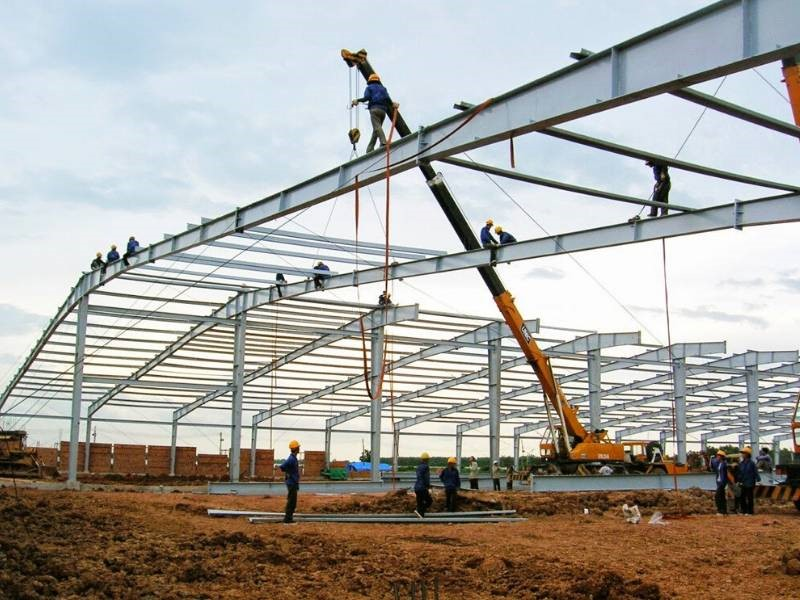
\includegraphics[width=186mm]{../../public/about1.jpg}};
  \fill[TTCDeepNavy, opacity=0.86] (0,0) rectangle (68,64);
  \fill[TTCDeepNavy, opacity=0.28] (68,0) rectangle (92,64);
  \node[anchor=west, text width=54mm, align=left, text=white] at (8,42) {
    {\fontsize{7}{8}\selectfont\bfseries\color{TTCCyan} STRATEGIC PEB NETWORK}\\[1.3mm]
    {\fontsize{19}{21}\selectfont\bfseries 30.000 TẤN}\\[-0.4mm]
    {\fontsize{8}{9.5}\selectfont\bfseries\color{TTCCyan} NĂNG LỰC CUNG ỨNG / NĂM}\\[1.8mm]
    {\fontsize{7}{8.6}\selectfont\color{white!82!gray}
    TTC làm chủ thiết kế, Shop Drawing và quyền phê duyệt xuất xưởng.}
  };
  \node[
    anchor=south east, rounded corners=3pt,
    fill=white, fill opacity=0.94, text opacity=1,
    draw=TTCCyan, line width=0.65pt,
    minimum width=55mm, minimum height=14mm, align=center
  ] at (179,7) {
    {\fontsize{9.5}{11}\selectfont\bfseries\color{TTCBlue} >20.000 m\textsuperscript{2} • RESIDENT QC}\\[0.6mm]
    {\fontsize{6.5}{7.8}\selectfont\color{TTCTextDark}Partner factory footprint • TTC supervision}
  };
  \draw[white, line width=1pt, rounded corners=3pt] (0.6,0.6) rectangle (185.4,63.4);
  \draw[TTCBorder, line width=0.65pt, rounded corners=3pt] (0,0) rectangle (186,64);
\end{tikzpicture}

\vspace{3mm}

% SIX-STAGE FABRICATION FLOW
\noindent
\begin{tikzpicture}[x=1mm,y=1mm]
  \path[use as bounding box] (0,0) rectangle (186,53);
  \node[anchor=west] at (0,48) {
    {\fontsize{7}{8}\selectfont\bfseries\color{TTCCyan} FABRICATION FLOW}\quad
    {\fontsize{9.5}{11}\selectfont\bfseries\color{TTCBlue} SÁU CÔNG ĐOẠN GIA CÔNG KHÉP KÍN}
  };
  \draw[TTCBlue!30!white, line width=0.85pt] (15,31) -- (171,31);

  \foreach \x/\num in {15/01,46/02,77/03,108/04,139/05,171/06}{
    \fill[white] (\x,31) circle (4.8);
    \draw[TTCBlue!48!white, line width=0.75pt] (\x,31) circle (4.8);
    \node[text=TTCBlue, font=\fontsize{6.8}{8}\selectfont\bfseries] at (\x,31) {\num};
  }
  \fill[TTCRed] (171,31) circle (4.8);
  \node[text=white, font=\fontsize{6.8}{8}\selectfont\bfseries] at (171,31) {06};

  \node[align=center, text width=25mm] at (15,13) {
    {\fontsize{8}{9.2}\selectfont\bfseries\color{TTCBlue} CNC CUTTING}\\[0.6mm]
    {\fontsize{6.3}{7.5}\selectfont Plasma • bevel}
  };
  \node[align=center, text width=25mm] at (46,13) {
    {\fontsize{8}{9.2}\selectfont\bfseries\color{TTCBlue} FIT-UP}\\[0.6mm]
    {\fontsize{6.3}{7.5}\selectfont Hydraulic jig}
  };
  \node[align=center, text width=25mm] at (77,13) {
    {\fontsize{8}{9.2}\selectfont\bfseries\color{TTCBlue} SAW WELD}\\[0.6mm]
    {\fontsize{6.3}{7.5}\selectfont AWS D1.1}
  };
  \node[align=center, text width=25mm] at (108,13) {
    {\fontsize{8}{9.2}\selectfont\bfseries\color{TTCBlue} STRAIGHTEN}\\[0.6mm]
    {\fontsize{6.3}{7.5}\selectfont Hydraulic press}
  };
  \node[align=center, text width=25mm] at (139,13) {
    {\fontsize{8}{9.2}\selectfont\bfseries\color{TTCBlue} BLASTING}\\[0.6mm]
    {\fontsize{6.3}{7.5}\selectfont Sa 2.5}
  };
  \node[align=center, text width=25mm] at (171,13) {
    {\fontsize{8}{9.2}\selectfont\bfseries\color{TTCRed} COATING}\\[0.6mm]
    {\fontsize{6.3}{7.5}\selectfont Epoxy • fireproof}
  };
\end{tikzpicture}

\vspace{3mm}

% QUALITY GATES
\noindent
\begin{tikzpicture}[x=1mm,y=1mm]
  \path[use as bounding box] (0,0) rectangle (186,53);

  \fill[white, rounded corners=4pt] (0,0) rectangle (58,53);
  \draw[TTCBorder, line width=0.65pt, rounded corners=4pt] (0,0) rectangle (58,53);
  \node[anchor=north west, text width=48mm, align=left] at (5,47) {
    {\fontsize{7}{8}\selectfont\bfseries\color{TTCCyan} QUALITY GATE 01}\\[0.8mm]
    {\fontsize{10}{11.5}\selectfont\bfseries\color{TTCBlue} MATERIAL RELEASE}\\[1.3mm]
    {\fontsize{7}{8.5}\selectfont\color{TTCTextDark}
    \textcolor{TTCCyan}{\faCheckCircle}\ MTC, CO/CQ và truy xuất lô thép.\\[0.7mm]
    \textcolor{TTCCyan}{\faCheckCircle}\ Q345B • SS400 • ASTM A572 Gr.50.\\[0.7mm]
    \textcolor{TTCCyan}{\faCheckCircle}\ Thí nghiệm cơ lý độc lập.}
  };

  \fill[TTCLightBlue, rounded corners=4pt] (64,0) rectangle (122,53);
  \draw[TTCBlue!50!white, line width=0.7pt, rounded corners=4pt] (64,0) rectangle (122,53);
  \node[anchor=north west, text width=48mm, align=left] at (69,47) {
    {\fontsize{7}{8}\selectfont\bfseries\color{TTCCyan} QUALITY GATE 02}\\[0.8mm]
    {\fontsize{10}{11.5}\selectfont\bfseries\color{TTCBlue} WELD ACCEPTANCE}\\[1.3mm]
    {\fontsize{7}{8.5}\selectfont\color{TTCTextDark}
    \textcolor{TTCBlue}{\faCheckCircle}\ WPS/PQR được phê duyệt.\\[0.7mm]
    \textcolor{TTCBlue}{\faCheckCircle}\ Thợ hàn chứng chỉ 3G/4G/6G.\\[0.7mm]
    \textcolor{TTCBlue}{\faCheckCircle}\ NDT UT/MT mối hàn chịu lực.}
  };

  \fill[white, rounded corners=4pt] (128,0) rectangle (186,53);
  \draw[TTCRed!65!white, line width=0.75pt, rounded corners=4pt] (128,0) rectangle (186,53);
  \node[anchor=north west, text width=48mm, align=left] at (133,47) {
    {\fontsize{7}{8}\selectfont\bfseries\color{TTCRed} QUALITY GATE 03}\\[0.8mm]
    {\fontsize{10}{11.5}\selectfont\bfseries\color{TTCBlue} FINISH \& RELEASE}\\[1.3mm]
    {\fontsize{7}{8.5}\selectfont\color{TTCTextDark}
    \textcolor{TTCRed}{\faCheckCircle}\ Làm sạch Sa 2.5 theo ISO 8501-1.\\[0.7mm]
    \textcolor{TTCRed}{\faCheckCircle}\ DFT bằng Elcometer.\\[0.7mm]
    \textcolor{TTCRed}{\faCheckCircle}\ Sơn Epoxy và chống cháy PCCC.}
  };
\end{tikzpicture}

\vspace{3mm}

% TTC RELEASE AUTHORITY
\noindent
\begin{tikzpicture}[x=1mm,y=1mm]
  \path[use as bounding box] (0,0) rectangle (186,30);
  \fill[TTCLightBlue, rounded corners=4pt] (0,0) rectangle (186,30);
  \draw[TTCBorder, line width=0.65pt, rounded corners=4pt] (0,0) rectangle (186,30);
  \node[anchor=west, align=left] at (6,15) {
    {\fontsize{7}{8}\selectfont\bfseries\color{TTCCyan} TTC CONTROL MODEL}\\[0.7mm]
    {\fontsize{9.3}{10.8}\selectfont\bfseries\color{TTCBlue} QUYỀN PHÊ DUYỆT XUẤT XƯỞNG}
  };
  \node[text=TTCRed] at (55,15) {\faChevronRight};
  \node[align=center] at (76,15) {
    {\fontsize{8.5}{10}\selectfont\bfseries\color{TTCBlue} DESIGN \& SHOP}\\[0.5mm]
    {\fontsize{6.3}{7.5}\selectfont TTC engineering}
  };
  \node[text=TTCRed] at (97,15) {\faChevronRight};
  \node[align=center] at (117,15) {
    {\fontsize{8.5}{10}\selectfont\bfseries\color{TTCBlue} RESIDENT QC}\\[0.5mm]
    {\fontsize{6.3}{7.5}\selectfont At partner factory}
  };
  \node[text=TTCRed] at (137,15) {\faChevronRight};
  \node[align=center] at (158,15) {
    {\fontsize{8.5}{10}\selectfont\bfseries\color{TTCRed} RELEASE NOTE}\\[0.5mm]
    {\fontsize{6.3}{7.5}\selectfont Ready for erection}
  };
\end{tikzpicture}
\vfill
\noindent\makebox[\linewidth][c]{%
  \begin{tikzpicture}[x=1mm,y=1mm]
    \path[use as bounding box] (0,0) rectangle (210,9);
    \begin{scope}[yshift=-20mm]
    \fill[TTCDeepNavy] (0,0) rectangle (210,8);
    \fill[TTCCyan] (0,8) rectangle (210,9);
    \node[anchor=west, text=white, font=\fontsize{6.8}{8}\selectfont]
      at (12,4) {\faPhone*\ +84 976 447 766 \quad\textbullet\quad \faEnvelope\ info@tanthanhcongjsc.com \quad\textbullet\quad \faGlobe\ https://tanthanhcongjsc.com};
    \node[anchor=east, text=white, font=\fontsize{7}{8}\selectfont\bfseries]
      at (198,4) {Trang 11};
    \end{scope}
  \end{tikzpicture}%
}
\end{minipage}
\newpage

% ============================================================
% TRANG 12: THIẾT BỊ THEO GÓI HUY ĐỘNG
% ============================================================
\pageheaderbar{THIẾT BỊ CƠ GIỚI \& HUY ĐỘNG HIỆN TRƯỜNG}{Trang 12}
\pagefooterbar{Trang 12}

\begin{tikzpicture}[remember picture, overlay]
  \fill[TTCLightBlue]
    ([xshift=137mm,yshift=-31mm]current page.north west) --
    ([xshift=210mm,yshift=-31mm]current page.north west) --
    ([xshift=210mm,yshift=-104mm]current page.north west) -- cycle;
  \draw[TTCBlue!8!white, line width=12pt]
    ([xshift=151mm,yshift=42mm]current page.south west) --
    ([xshift=205mm,yshift=96mm]current page.south west);
  \draw[TTCRed!8!white, line width=3pt]
    ([xshift=160mm,yshift=42mm]current page.south west) --
    ([xshift=205mm,yshift=87mm]current page.south west);
  % Faint industrial mobilization silhouette — replaces the old square grid
  \begin{scope}[shift={(current page.south west)},x=1mm,y=1mm,opacity=.48]
    \draw[TTCBlue!18!white, line width=.7pt] (12,13) -- (198,13);
    \fill[TTCBlue!2!white] (14,13) -- (14,34) -- (34,43) -- (54,34) --
      (54,13) -- cycle;
    \draw[TTCBlue!17!white, line width=.65pt] (14,13) -- (14,34) -- (34,43) --
      (54,34) -- (54,13);
    \foreach \x in {19,27,35,43,51}{\draw[TTCBlue!13!white] (\x,13) -- (\x,34);}
    \fill[TTCBlue!2!white] (61,13) rectangle (133,31);
    \draw[TTCBlue!17!white, line width=.65pt] (61,13) rectangle (133,31);
    \foreach \x in {73,85,97,109,121}{\draw[TTCBlue!12!white] (\x,13) -- (\x,31);}
    \draw[TTCBlue!17!white] (61,22) -- (133,22);
    % tower crane / lifting cue
    \draw[TTCBlue!20!white, line width=.85pt] (151,13) -- (151,51);
    \draw[TTCBlue!18!white] (146,13) -- (151,51) -- (156,13);
    \draw[TTCBlue!20!white, line width=.85pt] (151,48) -- (198,48);
    \draw[TTCBlue!17!white] (151,48) -- (177,39) -- (198,48);
    \draw[TTCRed!22!white, line width=.7pt] (184,48) -- (184,25);
    \draw[TTCRed!22!white] (181,25) -- (187,25);
  \end{scope}
\end{tikzpicture}

\begin{minipage}[t][246mm]{\textwidth}
\secbrand{Năng Lực Thiết Bị Theo Gói Huy Động}{Right Equipment, Right Workfront, Right Time}

{\fontsize{15}{17}\selectfont\bfseries\color{TTCBlue}
43+ THIẾT BỊ • 4 GÓI NHIỆM VỤ • MỘT ĐẦU MỐI ĐIỀU PHỐI\par}
\vspace{1mm}
{\fontsize{7.5}{9}\selectfont\color{TTCTextMuted}
Danh mục được tinh gọn theo năng lực thực thi, ưu tiên khả năng điều động, kiểm định và hiệu suất tại công trường.\par}
\vspace{3mm}

% HERO — SITE MOBILIZATION
\noindent
\begin{tikzpicture}[x=1mm,y=1mm]
  \path[use as bounding box] (0,0) rectangle (186,58);
  \clip[rounded corners=3pt] (0,0) rectangle (186,58);
  \node[anchor=center, inner sep=0pt] at (93,29)
    {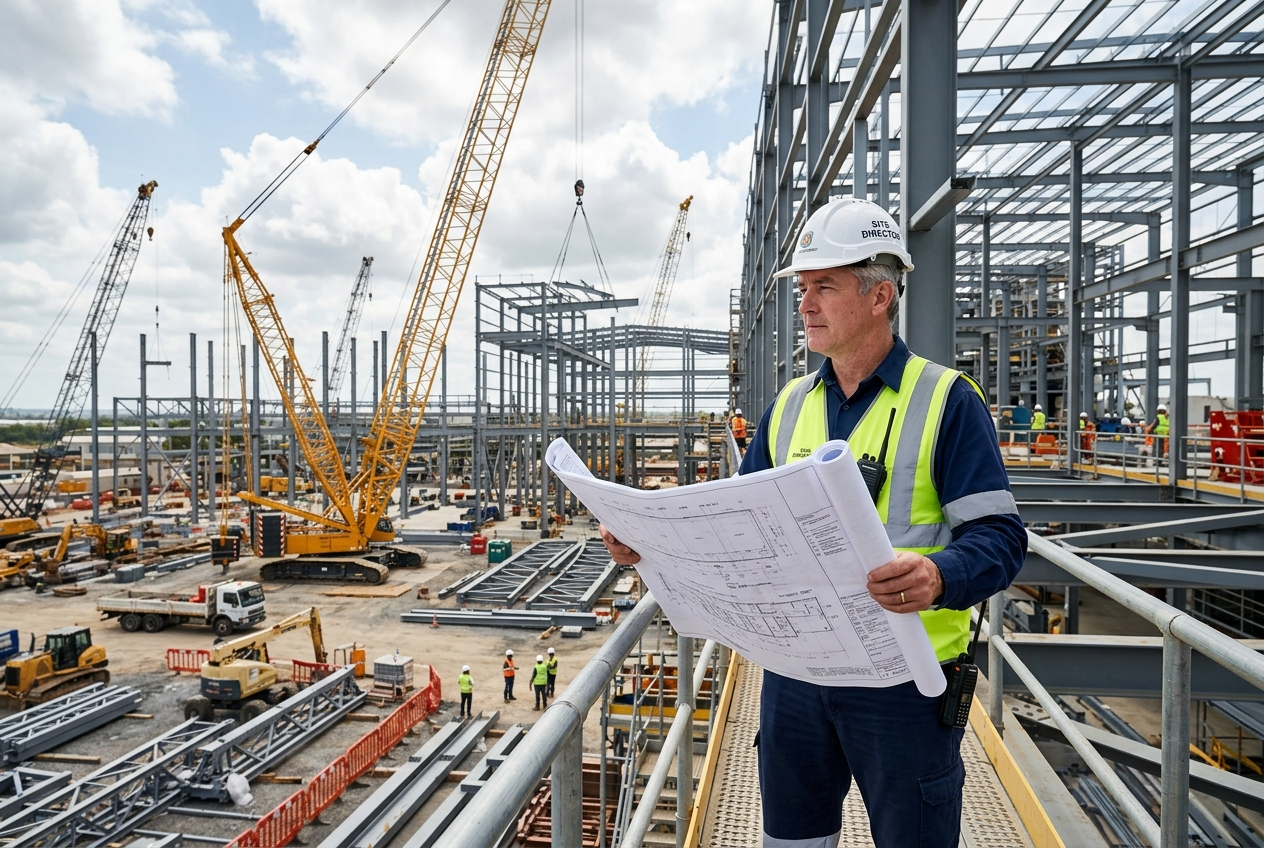
\includegraphics[width=186mm]{../../public/c_level_site_inspection.jpg}};
  \fill[TTCDeepNavy, opacity=0.88] (0,0) rectangle (68,58);
  \fill[TTCDeepNavy, opacity=0.35] (68,0) rectangle (94,58);
  \node[anchor=west, text width=54mm, align=left, text=white] at (8,38) {
    {\fontsize{7}{8}\selectfont\bfseries\color{TTCCyan} MOBILIZATION CONTROL}\\[1.5mm]
    {\fontsize{21}{22}\selectfont\bfseries 43+}\\[-0.5mm]
    {\fontsize{9}{10.5}\selectfont\bfseries THIẾT BỊ SẴN SÀNG}\\[1.7mm]
    {\fontsize{7}{8.5}\selectfont\color{white!82!gray}
    Điều phối theo đường găng và mặt bằng thi công, không dàn trải nguồn lực.}
  };
  \node[rounded corners=2pt, fill=white, text=TTCBlue, align=center,
        minimum width=31mm, minimum height=16mm] at (129,17) {
    {\fontsize{13}{14}\selectfont\bfseries 100T}\\[-0.4mm]
    {\fontsize{6.2}{7.4}\selectfont SỨC NÂNG TỐI ĐA}
  };
  \node[rounded corners=2pt, fill=TTCRed, text=white, align=center,
        minimum width=35mm, minimum height=16mm] at (167,17) {
    {\fontsize{11}{12}\selectfont\bfseries 100\%}\\[-0.4mm]
    {\fontsize{6.2}{7.4}\selectfont KIỂM ĐỊNH HIỆU LỰC}
  };
\end{tikzpicture}

\vspace{3mm}

% FOUR MISSION PACKAGES
\noindent
\begin{tikzpicture}[x=1mm,y=1mm]
  \path[use as bounding box] (0,0) rectangle (186,50);
  \foreach \x/\accent in {0/TTCRed,47.5/TTCCyan,95/TTCBlue,142.5/TTCGold}{
    \fill[white, rounded corners=2pt] (\x,0) rectangle +(43.5,50);
    \draw[TTCBorder, rounded corners=2pt, line width=.55pt] (\x,0) rectangle +(43.5,50);
    \fill[\accent, rounded corners=2pt] (\x,46) rectangle +(43.5,4);
  }
  \node[anchor=north west, text width=35mm, align=left] at (4,43) {
    {\fontsize{15}{16}\selectfont\bfseries\color{TTCRed} 20}\\[-.5mm]
    {\fontsize{7.4}{8.5}\selectfont\bfseries\color{TTCBlue} NÂNG HẠ \& TIẾP CẬN}\\[1mm]
    {\fontsize{6.6}{8}\selectfont\color{TTCTextDark}
    06 cẩu tự hành 25--100T\newline
    14 xe Boomlift 18--28m\newline
    Lắp dựng thép, mái và MEP trên cao.}
  };
  \node[anchor=north west, text width=35mm, align=left] at (51.5,43) {
    {\fontsize{15}{16}\selectfont\bfseries\color{TTCCyan} 12}\\[-.5mm]
    {\fontsize{7.4}{8.5}\selectfont\bfseries\color{TTCBlue} NỀN \& BÊ TÔNG}\\[1mm]
    {\fontsize{6.6}{8}\selectfont\color{TTCTextDark}
    08 máy xúc, lu nền\newline
    04 bơm và xe bồn bê tông\newline
    Hạ tầng, nền móng và sàn công nghiệp.}
  };
  \node[anchor=north west, text width=35mm, align=left] at (99,43) {
    {\fontsize{15}{16}\selectfont\bfseries\color{TTCBlue} 02}\\[-.5mm]
    {\fontsize{7.4}{8.5}\selectfont\bfseries\color{TTCBlue} MÁI \& BAO CHE}\\[1mm]
    {\fontsize{6.6}{8}\selectfont\color{TTCTextDark}
    02 dàn cán tôn di động\newline
    Cliplock / Seamlock tại chỗ\newline
    Dải tôn dài, hạn chế mối nối và thấm dột.}
  };
  \node[anchor=north west, text width=35mm, align=left] at (146.5,43) {
    {\fontsize{15}{16}\selectfont\bfseries\color{TTCGold} 09}\\[-.5mm]
    {\fontsize{7.4}{8.5}\selectfont\bfseries\color{TTCBlue} TRẮC ĐẠC \& QA}\\[1mm]
    {\fontsize{6.6}{8}\selectfont\color{TTCTextDark}
    09 bộ Leica / Laser 3D\newline
    Kiểm soát tim trục và cao độ\newline
    Sai số mục tiêu dưới 2mm.}
  };
\end{tikzpicture}

\vspace{3mm}

% DEPLOYMENT SEQUENCE
\noindent
\begin{tikzpicture}[x=1mm,y=1mm]
  \path[use as bounding box] (0,0) rectangle (186,42);
  \fill[TTCLightBlue, rounded corners=3pt] (0,0) rectangle (186,42);
  \draw[TTCBorder, rounded corners=3pt, line width=.6pt] (0,0) rectangle (186,42);
  \node[anchor=west, font=\fontsize{8}{9.5}\selectfont\bfseries, text=TTCBlue] at (7,35)
    {\faClock\quad NHỊP HUY ĐỘNG THEO ĐƯỜNG GĂNG DỰ ÁN};
  \draw[TTCBlue!35!white, line width=1pt] (19,19) -- (167,19);
  \foreach \x/\n/\t/\s in {
    21/01/NỀN MÓNG/Khảo sát • đào đắp • bê tông,
    69/02/KẾT CẤU/Cẩu lắp • tiếp cận trên cao,
    117/03/BAO CHE/Cán tôn • mái • hoàn thiện,
    165/04/NGHIỆM THU/Trắc đạc • kiểm định • bàn giao}{
      \fill[white] (\x,19) circle (4.7);
      \draw[TTCBlue, line width=.8pt] (\x,19) circle (4.7);
      \node[font=\fontsize{6.8}{8}\selectfont\bfseries, text=TTCRed] at (\x,19) {\n};
      \node[anchor=north, align=center, text width=38mm] at (\x,12) {
        {\fontsize{6.8}{8}\selectfont\bfseries\color{TTCBlue} \t}\\[-.3mm]
        {\fontsize{5.8}{7}\selectfont\color{TTCTextMuted} \s}
      };
  }
\end{tikzpicture}

\vspace{3mm}

% ASSURANCE STRIP
\noindent
\begin{tikzpicture}[x=1mm,y=1mm]
  \path[use as bounding box] (0,0) rectangle (186,29);
  \fill[TTCDeepNavy, rounded corners=3pt] (0,0) rectangle (186,29);
  \foreach \x in {46.5,93,139.5}{\draw[white!35!gray] (\x,6) -- (\x,23);}
  \node[align=center, text=white] at (23.25,15) {{\fontsize{9}{10}\selectfont\bfseries\color{TTCRed} 12 GIỜ}\\[-.3mm]{\fontsize{6.2}{7.4}\selectfont Điều Động Khẩn Cấp}};
  \node[align=center, text=white] at (69.75,15) {{\fontsize{9}{10}\selectfont\bfseries\color{TTCCyan} CHỨNG CHỈ}\\[-.3mm]{\fontsize{6.2}{7.4}\selectfont Vận Hành Đúng Chuẩn}};
  \node[align=center, text=white] at (116.25,15) {{\fontsize{9}{10}\selectfont\bfseries BẢO DƯỠNG}\\[-.3mm]{\fontsize{6.2}{7.4}\selectfont Theo Khuyến Nghị Hãng}};
  \node[align=center, text=white] at (162.75,15) {{\fontsize{9}{10}\selectfont\bfseries\color{TTCGold} NHẬT KÝ SỐ}\\[-.3mm]{\fontsize{6.2}{7.4}\selectfont Trạng Thái Theo Thời Gian}};
\end{tikzpicture}
\end{minipage}
\newpage

% ============================================================
% TRANG 13: QUẢN TRỊ DỰ ÁN STAGE-GATE
% ============================================================
\pagefooterbar{Trang 13}

\begin{tikzpicture}[remember picture, overlay]
  \fill[TTCLightBlue]
    ([xshift=118mm,yshift=-32mm]current page.north west) --
    ([xshift=210mm,yshift=-32mm]current page.north west) --
    ([xshift=210mm,yshift=-118mm]current page.north west) -- cycle;
  \node[opacity=.035, font=\fontsize{62}{64}\selectfont\bfseries, text=TTCBlue,
        rotate=90] at ([xshift=-10mm,yshift=18mm]current page.east) {GATE};
  % Four translucent decision chevrons continue the process into the footer
  \begin{scope}[shift={(current page.south west)},x=1mm,y=1mm,opacity=.42]
    \foreach \x/\c in {15/TTCRed,60/TTCCyan,105/TTCBlue,150/TTCGold}{
      \fill[\c!7!white] (\x,14) -- ++(31,0) -- ++(10,14) -- ++(-10,14) --
        ++(-31,0) -- ++(10,-14) -- cycle;
    }
    \node[text=TTCRed!35!white,font=\fontsize{7}{8}\selectfont\bfseries] at (35,28) {DEFINE};
    \node[text=TTCCyan!40!white,font=\fontsize{7}{8}\selectfont\bfseries] at (80,28) {ENGINEER};
    \node[text=TTCBlue!35!white,font=\fontsize{7}{8}\selectfont\bfseries] at (125,28) {BUILD};
    \node[text=TTCGold!40!white,font=\fontsize{7}{8}\selectfont\bfseries] at (170,28) {HANDOVER};
  \end{scope}
\end{tikzpicture}

\begin{minipage}[t][246mm]{\textwidth}
\pageheaderbar{QUẢN TRỊ DỰ ÁN EPC THEO STAGE-GATE}{Trang 13}
\secbrand{Quản Trị Dự Án EPC Theo 4 Pha Kiểm Soát}{FIDIC Turnkey Governance, Decision Gates \& Single-Point Accountability}

{\fontsize{15}{17}\selectfont\bfseries\color{TTCBlue}
MỖI GIAI ĐOẠN CÓ ĐẦU RA • MỖI CHUYỂN PHA CÓ PHÊ DUYỆT\par}
\vspace{1mm}
{\fontsize{7.5}{9}\selectfont\color{TTCTextMuted}
Tám bước triển khai được gom thành bốn pha quản trị, giúp Chủ đầu tư nhìn rõ quyết định, trách nhiệm và trạng thái dự án.\par}
\vspace{3mm}

% FOUR PHASES / FOUR GATES
\noindent
\begin{tikzpicture}[x=1mm,y=1mm]
  \path[use as bounding box] (0,0) rectangle (186,103);

  % PHASE 01
  \fill[white, rounded corners=2pt] (0,0) rectangle (43.5,103);
  \draw[TTCBorder, rounded corners=2pt, line width=.65pt] (0,0) rectangle (43.5,103);
  \fill[TTCDeepNavy, rounded corners=2pt] (0,84) rectangle (43.5,103);
  \node[anchor=west, text=white] at (4,94) {{\fontsize{7}{8}\selectfont 01}\quad{\fontsize{10}{11}\selectfont\bfseries DEFINE}};
  \node[anchor=north west, text width=35.5mm, align=left] at (4,79) {
    {\fontsize{7}{8.5}\selectfont\bfseries\color{TTCRed} 01 • KHẢO SÁT \& BRIEF}\\[.7mm]
    {\fontsize{6.2}{7.5}\selectfont\color{TTCTextDark}Địa chất, địa hình 3D; yêu cầu công năng và báo cáo tiền khả thi.}\\[3mm]
    {\fontsize{7}{8.5}\selectfont\bfseries\color{TTCBlue} 02 • PHÁP LÝ \& QUY HOẠCH}\\[.7mm]
    {\fontsize{6.2}{7.5}\selectfont\color{TTCTextDark}Quy hoạch 1/500, ĐTM, PCCC, giấy phép xây dựng và cơ sở thiết kế.}
  };
  \fill[TTCRed!8!white] (3.5,5) rectangle (40,17);
  \node[align=center, text=TTCRed] at (21.75,11) {{\fontsize{6}{7}\selectfont\bfseries GATE A}\\[-.2mm]{\fontsize{5.7}{6.7}\selectfont Basis Approved}};

  % PHASE 02
  \fill[white, rounded corners=2pt] (47.5,0) rectangle (91,103);
  \draw[TTCBorder, rounded corners=2pt, line width=.65pt] (47.5,0) rectangle (91,103);
  \fill[TTCBlue, rounded corners=2pt] (47.5,84) rectangle (91,103);
  \node[anchor=west, text=white] at (51.5,94) {{\fontsize{7}{8}\selectfont 02}\quad{\fontsize{10}{11}\selectfont\bfseries ENGINEER}};
  \node[anchor=north west, text width=35.5mm, align=left] at (51.5,79) {
    {\fontsize{7}{8.5}\selectfont\bfseries\color{TTCCyan} 03 • VALUE ENGINEERING}\\[.7mm]
    {\fontsize{6.2}{7.5}\selectfont\color{TTCTextDark}BIM LOD 400, tối ưu kết cấu, phối hợp bộ môn và kiểm soát xung đột.}\\[3mm]
    {\fontsize{7}{8.5}\selectfont\bfseries\color{TTCBlue} 04 • PROCUREMENT \& PEB}\\[.7mm]
    {\fontsize{6.2}{7.5}\selectfont\color{TTCTextDark}Vật tư Tier-1, Shop Drawing, kế hoạch mua sắm và QC thường trú tại xưởng.}
  };
  \fill[TTCCyan!10!white] (51,5) rectangle (87.5,17);
  \node[align=center, text=TTCBlue] at (69.25,11) {{\fontsize{6}{7}\selectfont\bfseries GATE B}\\[-.2mm]{\fontsize{5.7}{6.7}\selectfont Design Freeze}};

  % PHASE 03
  \fill[white, rounded corners=2pt] (95,0) rectangle (138.5,103);
  \draw[TTCBorder, rounded corners=2pt, line width=.65pt] (95,0) rectangle (138.5,103);
  \fill[TTCCyan!85!TTCBlue, rounded corners=2pt] (95,84) rectangle (138.5,103);
  \node[anchor=west, text=white] at (99,94) {{\fontsize{7}{8}\selectfont 03}\quad{\fontsize{10}{11}\selectfont\bfseries BUILD}};
  \node[anchor=north west, text width=35.5mm, align=left] at (99,79) {
    {\fontsize{7}{8.5}\selectfont\bfseries\color{TTCRed} 05 • GROUND \& INFRA}\\[.7mm]
    {\fontsize{6.2}{7.5}\selectfont\color{TTCTextDark}Cọc, móng, nền, hạ tầng kỹ thuật và các workfront bàn giao theo ITP.}\\[3mm]
    {\fontsize{7}{8.5}\selectfont\bfseries\color{TTCBlue} 06 • STRUCTURE \& MEP}\\[.7mm]
    {\fontsize{6.2}{7.5}\selectfont\color{TTCTextDark}Kết cấu thép, bao che, MEP, PCCC và kiểm soát tiến độ đường găng.}
  };
  \fill[TTCBlue!8!white] (98.5,5) rectangle (135,17);
  \node[align=center, text=TTCBlue] at (116.75,11) {{\fontsize{6}{7}\selectfont\bfseries GATE C}\\[-.2mm]{\fontsize{5.7}{6.7}\selectfont Ready To Test}};

  % PHASE 04
  \fill[white, rounded corners=2pt] (142.5,0) rectangle (186,103);
  \draw[TTCBorder, rounded corners=2pt, line width=.65pt] (142.5,0) rectangle (186,103);
  \fill[TTCGold, rounded corners=2pt] (142.5,84) rectangle (186,103);
  \node[anchor=west, text=white] at (146.5,94) {{\fontsize{7}{8}\selectfont 04}\quad{\fontsize{10}{11}\selectfont\bfseries HANDOVER}};
  \node[anchor=north west, text width=35.5mm, align=left] at (146.5,79) {
    {\fontsize{7}{8.5}\selectfont\bfseries\color{TTCRed} 07 • TEST \& APPROVAL}\\[.7mm]
    {\fontsize{6.2}{7.5}\selectfont\color{TTCTextDark}Nghiệm thu ITP, PCCC, chạy thử đơn động và liên động hệ thống.}\\[3mm]
    {\fontsize{7}{8.5}\selectfont\bfseries\color{TTCBlue} 08 • HANDOVER \& O\&M}\\[.7mm]
    {\fontsize{6.2}{7.5}\selectfont\color{TTCTextDark}As-built, Digital Twin, đào tạo vận hành, bảo hành và kế hoạch bảo trì.}
  };
  \fill[TTCGold!12!white] (146,5) rectangle (182.5,17);
  \node[align=center, text=TTCGold!80!black] at (164.25,11) {{\fontsize{6}{7}\selectfont\bfseries GATE D}\\[-.2mm]{\fontsize{5.7}{6.7}\selectfont Ready To Operate}};

  % TRANSITION MARKERS
  \foreach \x/\l in {45.5/A,93/B,140.5/C}{
    \fill[white] (\x,51) circle (3.8);
    \draw[TTCRed, line width=.8pt] (\x,51) circle (3.8);
    \node[text=TTCRed, font=\fontsize{5.5}{6}\selectfont\bfseries] at (\x,51) {\l};
  }
\end{tikzpicture}

\vspace{3mm}

% GOVERNANCE SPINE
\noindent
\begin{tikzpicture}[x=1mm,y=1mm]
  \path[use as bounding box] (0,0) rectangle (186,43);
  \fill[TTCLightBlue, rounded corners=3pt] (0,0) rectangle (186,43);
  \draw[TTCBorder, rounded corners=3pt, line width=.6pt] (0,0) rectangle (186,43);
  \node[anchor=west, text=TTCBlue, font=\fontsize{8}{9.5}\selectfont\bfseries] at (7,35)
    {\faProjectDiagram\quad GOVERNANCE SPINE — MỘT HỆ QUẢN TRỊ XUYÊN SUỐT};
  \foreach \x in {46.5,93,139.5}{\draw[TTCBorder] (\x,6) -- (\x,28);}
  \node[align=center, text width=39mm] at (23.25,17) {{\fontsize{7}{8}\selectfont\bfseries\color{TTCRed} PROJECT DIRECTOR}\\[-.2mm]{\fontsize{5.8}{7}\selectfont\color{TTCTextMuted}Một đầu mối chịu trách nhiệm đầu ra}};
  \node[align=center, text width=39mm] at (69.75,17) {{\fontsize{7}{8}\selectfont\bfseries\color{TTCBlue} CPM BASELINE}\\[-.2mm]{\fontsize{5.8}{7}\selectfont\color{TTCTextMuted}Đường găng và look-ahead hàng tuần}};
  \node[align=center, text width=39mm] at (116.25,17) {{\fontsize{7}{8}\selectfont\bfseries\color{TTCCyan} COMMON DATA ENV.}\\[-.2mm]{\fontsize{5.8}{7}\selectfont\color{TTCTextMuted}Bản vẽ, RFI, ITP có truy vết}};
  \node[align=center, text width=39mm] at (162.75,17) {{\fontsize{7}{8}\selectfont\bfseries\color{TTCGold} FIDIC CONTROL}\\[-.2mm]{\fontsize{5.8}{7}\selectfont\color{TTCTextMuted}Scope, change và rủi ro hợp đồng}};
\end{tikzpicture}

\vspace{3mm}

% OUTCOME STRIP
\noindent
\begin{tikzpicture}[x=1mm,y=1mm]
  \path[use as bounding box] (0,0) rectangle (186,29);
  \fill[TTCDeepNavy, rounded corners=3pt] (0,0) rectangle (186,29);
  \foreach \x in {46.5,93,139.5}{\draw[white!35!gray] (\x,6) -- (\x,23);}
  \node[align=center, text=white] at (23.25,15) {{\fontsize{9}{10}\selectfont\bfseries\color{TTCRed} 8 BƯỚC}\\[-.3mm]{\fontsize{6.2}{7.4}\selectfont Trong 4 Pha Kiểm Soát}};
  \node[align=center, text=white] at (69.75,15) {{\fontsize{9}{10}\selectfont\bfseries\color{TTCCyan} 4 GATES}\\[-.3mm]{\fontsize{6.2}{7.4}\selectfont Quyết Định Có Điều Kiện}};
  \node[align=center, text=white] at (116.25,15) {{\fontsize{9}{10}\selectfont\bfseries FIDIC EPC}\\[-.3mm]{\fontsize{6.2}{7.4}\selectfont Chuẩn Hợp Đồng Quốc Tế}};
  \node[align=center, text=white] at (162.75,15) {{\fontsize{9}{10}\selectfont\bfseries\color{TTCGold} 24 THÁNG}\\[-.3mm]{\fontsize{6.2}{7.4}\selectfont Bảo Hành Toàn Diện}};
\end{tikzpicture}
\end{minipage}
\newpage

% ============================================================
% TRANG 14: EPC VALUE MODEL — ONE CONTRACT, ONE ACCOUNTABILITY
% ============================================================
\begin{tikzpicture}[remember picture, overlay]
  \fill[TTCLightBlue]
    ([xshift=132mm,yshift=-30mm]current page.north west) --
    ([xshift=210mm,yshift=-30mm]current page.north west) --
    ([xshift=210mm,yshift=-104mm]current page.north west) -- cycle;
  \draw[TTCBlue!7!white, line width=12pt]
    ([xshift=154mm,yshift=37mm]current page.south west) --
    ([xshift=205mm,yshift=88mm]current page.south west);
  \draw[TTCRed!8!white, line width=3pt]
    ([xshift=162mm,yshift=37mm]current page.south west) --
    ([xshift=205mm,yshift=80mm]current page.south west);
  % A light structural frame at the bottom — no square grid
  \begin{scope}[shift={(current page.south west)},x=1mm,y=1mm,opacity=.42]
    \draw[TTCBlue!17!white, line width=.7pt] (12,13) -- (198,13);
    \draw[TTCBlue!16!white] (17,13) -- (17,37) -- (47,50) -- (77,37) --
      (107,50) -- (137,37) -- (167,50) -- (197,37) -- (197,13);
    \foreach \x in {17,47,77,107,137,167,197}{\draw[TTCBlue!12!white] (\x,13) -- (\x,42);}
    \draw[TTCRed!18!white, line width=.7pt] (17,20) -- (197,20);
  \end{scope}
\end{tikzpicture}

\pagefooterbar{Trang 14}
\begin{minipage}[t][246mm]{\textwidth}
\pageheaderbar{GIẢI PHÁP TỔNG THẦU EPC \& VALUE ENGINEERING}{Trang 14}
\vspace{6mm}
\secbrand{Mô Hình Tổng Thầu EPC Tạo Giá Trị}{Fast-Track Delivery, Value Engineering \& Single-Point Accountability}

{\fontsize{15}{17}\selectfont\bfseries\color{TTCBlue}
NHANH HƠN • GỌN HƠN • ÍT RỦI RO HƠN\par}
\vspace{1mm}
{\fontsize{7.5}{9}\selectfont\color{TTCTextMuted}
TTC tích hợp pháp lý, thiết kế, mua sắm và thi công trong một hợp đồng — mọi quyết định cùng hướng tới hiệu quả đầu tư cuối cùng.\par}
\vspace{3mm}

% HERO — THE FACILITY AS ONE INTEGRATED SYSTEM
\noindent
\begin{tikzpicture}[x=1mm,y=1mm]
  \path[use as bounding box] (0,0) rectangle (186,66);
  \clip[rounded corners=3pt] (0,0) rectangle (186,66);
  \node[anchor=center, inner sep=0pt] at (93,33)
    {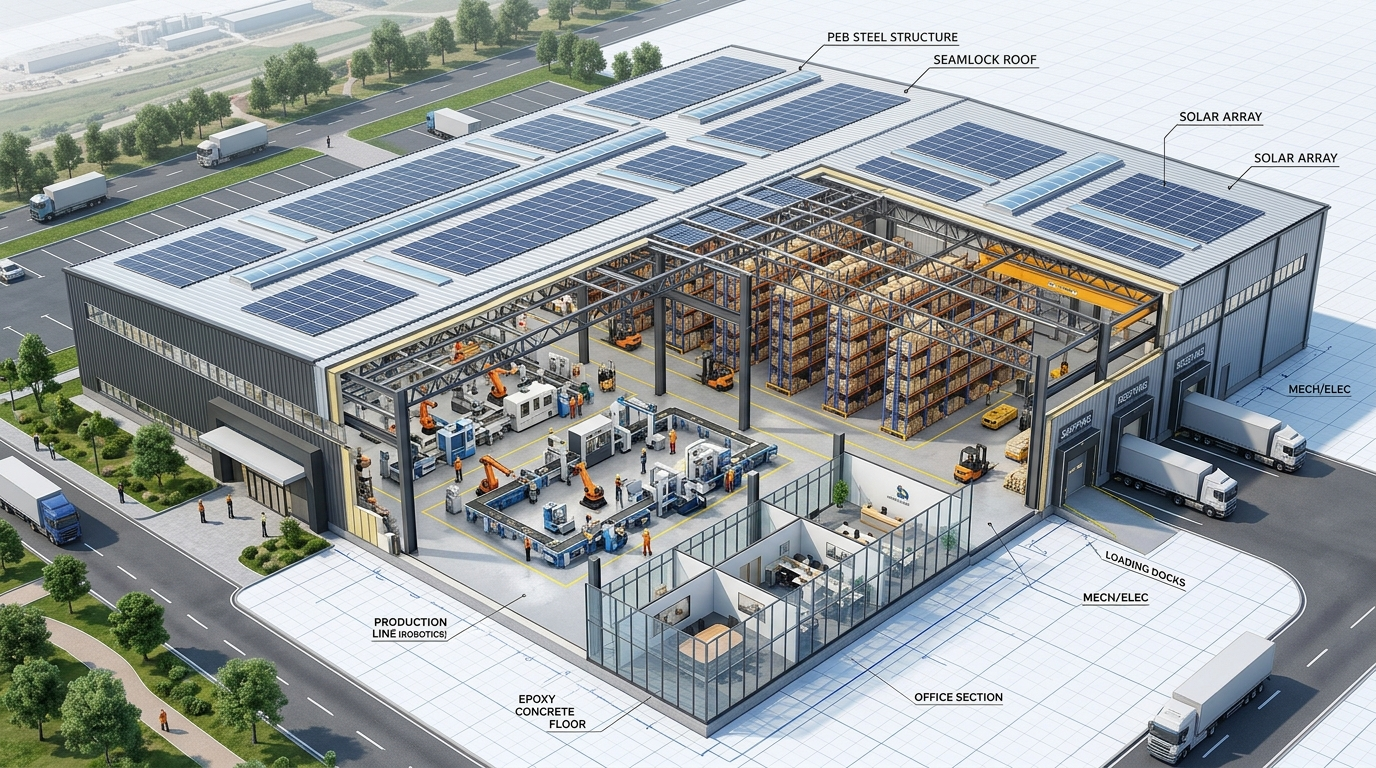
\includegraphics[width=186mm]{../../public/factory-tech-3d.jpg}};
  \fill[TTCDeepNavy, opacity=.88] (0,0) rectangle (66,66);
  \fill[TTCDeepNavy, opacity=.26] (66,0) rectangle (92,66);
  \node[anchor=west, text width=52mm, align=left, text=white] at (8,43) {
    {\fontsize{7}{8}\selectfont\bfseries\color{TTCCyan} TTC EPC VALUE MODEL}\\[1.3mm]
    {\fontsize{17}{19}\selectfont\bfseries ONE CONTRACT}\\[-.2mm]
    {\fontsize{10}{12}\selectfont\bfseries\color{TTCRed!85!white} ONE ACCOUNTABILITY}\\[1.7mm]
    {\fontsize{7}{8.5}\selectfont\color{white!82!gray}
    Một đầu mối kiểm soát phạm vi, ngân sách, tiến độ và chất lượng bàn giao.}
  };
  \node[rounded corners=2pt, fill=white, align=center, minimum width=29mm,
        minimum height=15mm] at (113,15) {
    {\fontsize{11}{12}\selectfont\bfseries\color{TTCRed} -15\%}\\[-.3mm]
    {\fontsize{5.8}{7}\selectfont\color{TTCBlue} KHỐI LƯỢNG THÉP}
  };
  \node[rounded corners=2pt, fill=white, align=center, minimum width=29mm,
        minimum height=15mm] at (145,15) {
    {\fontsize{11}{12}\selectfont\bfseries\color{TTCCyan} -60}\\[-.3mm]
    {\fontsize{5.8}{7}\selectfont\color{TTCBlue} NGÀY TIẾN ĐỘ}
  };
  \node[rounded corners=2pt, fill=TTCGold, text=white, align=center,
        minimum width=29mm, minimum height=15mm] at (177,15) {
    {\fontsize{11}{12}\selectfont\bfseries 0}\\[-.3mm]
    {\fontsize{5.8}{7}\selectfont XUNG ĐỘT MEP}
  };
\end{tikzpicture}

\vspace{3mm}

% SIX WORKSTREAMS — SIMPLE MEMORY LINE
\noindent
\begin{tikzpicture}[x=1mm,y=1mm]
  \path[use as bounding box] (0,0) rectangle (186,48);
  \fill[TTCLightBlue, rounded corners=3pt] (0,0) rectangle (186,48);
  \draw[TTCBorder, rounded corners=3pt, line width=.6pt] (0,0) rectangle (186,48);
  \node[anchor=west, text=TTCBlue, font=\fontsize{8}{9.5}\selectfont\bfseries] at (7,40)
    {\faProjectDiagram\quad SÁU DÒNG CÔNG VIỆC — MỘT CHUỖI GIÁ TRỊ};
  \draw[TTCBlue!35!white, line width=1pt] (14,23) -- (172,23);
  \foreach \x/\n/\t/\s in {
    16/01/DEFINE/Pháp lý \& brief,
    47/02/OPTIMIZE/VE \& BIM 5D,
    78/03/ENGINEER/Shop Drawing,
    109/04/FABRICATE/PEB \& supply,
    140/05/BUILD/Foundation \& MEP,
    171/06/OPERATE/Twin \& O\&M}{
      \fill[white] (\x,23) circle (4.6);
      \draw[TTCBlue, line width=.75pt] (\x,23) circle (4.6);
      \node[text=TTCRed,font=\fontsize{6.4}{7}\selectfont\bfseries] at (\x,23) {\n};
      \node[anchor=north,align=center,text width=27mm] at (\x,16) {
        {\fontsize{6.6}{7.8}\selectfont\bfseries\color{TTCBlue} \t}\\[-.2mm]
        {\fontsize{5.7}{6.8}\selectfont\color{TTCTextMuted} \s}
      };
  }
\end{tikzpicture}

\vspace{3mm}

% THREE SOURCES OF VALUE
\noindent
\begin{tikzpicture}[x=1mm,y=1mm]
  \path[use as bounding box] (0,0) rectangle (186,49);
  \foreach \x/\c in {0/TTCRed,63/TTCCyan,126/TTCGold}{
    \fill[white, rounded corners=2pt] (\x,0) rectangle +(60,49);
    \draw[TTCBorder, rounded corners=2pt, line width=.6pt] (\x,0) rectangle +(60,49);
    \fill[\c, rounded corners=2pt] (\x,45) rectangle +(60,4);
  }
  \node[anchor=north west, text width=50mm] at (5,40) {
    {\fontsize{8}{9.5}\selectfont\bfseries\color{TTCRed} 01 • DESIGN LESS}\\[1mm]
    {\fontsize{10}{11}\selectfont\bfseries\color{TTCBlue} TỐI ƯU KẾT CẤU}\\[1mm]
    {\fontsize{6.8}{8.2}\selectfont\color{TTCTextDark}
    Dầm Tapered theo nội lực, giảm tải xuống móng và bảo toàn hệ số an toàn.}
  };
  \node[anchor=north west, text width=50mm] at (68,40) {
    {\fontsize{8}{9.5}\selectfont\bfseries\color{TTCCyan} 02 • BUILD EARLIER}\\[1mm]
    {\fontsize{10}{11}\selectfont\bfseries\color{TTCBlue} CHẠY SONG SONG}\\[1mm]
    {\fontsize{6.8}{8.2}\selectfont\color{TTCTextDark}
    Thiết kế, gia công PEB và nền móng triển khai đồng thời theo đường găng.}
  };
  \node[anchor=north west, text width=50mm] at (131,40) {
    {\fontsize{8}{9.5}\selectfont\bfseries\color{TTCGold} 03 • CONTROL RISK}\\[1mm]
    {\fontsize{10}{11}\selectfont\bfseries\color{TTCBlue} KHÓA PHẠM VI}\\[1mm]
    {\fontsize{6.8}{8.2}\selectfont\color{TTCTextDark}
    BIM clash-check, release gate và hợp đồng Lump-sum hạn chế phát sinh.}
  };
\end{tikzpicture}

\vspace{3mm}

% KPI MEMORY STRIP
\noindent
\begin{tikzpicture}[x=1mm,y=1mm]
  \path[use as bounding box] (0,0) rectangle (186,29);
  \fill[TTCDeepNavy, rounded corners=3pt] (0,0) rectangle (186,29);
  \foreach \x in {46.5,93,139.5}{\draw[white!35!gray] (\x,6) -- (\x,23);}
  \node[align=center,text=white] at (23.25,15) {{\fontsize{9}{10}\selectfont\bfseries\color{TTCRed} TỐI ƯU CHI PHÍ}\\[-.3mm]{\fontsize{6.2}{7.4}\selectfont Value Engineering}};
  \node[align=center,text=white] at (69.75,15) {{\fontsize{9}{10}\selectfont\bfseries\color{TTCCyan} 45--60 NGÀY}\\[-.3mm]{\fontsize{6.2}{7.4}\selectfont Fast-Track Delivery}};
  \node[align=center,text=white] at (116.25,15) {{\fontsize{9}{10}\selectfont\bfseries 0 CLASH}\\[-.3mm]{\fontsize{6.2}{7.4}\selectfont BIM Coordination}};
  \node[align=center,text=white] at (162.75,15) {{\fontsize{9}{10}\selectfont\bfseries\color{TTCGold} LUMP-SUM}\\[-.3mm]{\fontsize{6.2}{7.4}\selectfont Budget Certainty}};
\end{tikzpicture}
\end{minipage}
\newpage

% ============================================================
% TRANG 15: DIGITAL THREAD — BIM, AI, DIGITAL TWIN
% ============================================================
\begin{tikzpicture}[remember picture, overlay]
  \fill[TTCLightBlue]
    ([xshift=122mm,yshift=-31mm]current page.north west) --
    ([xshift=210mm,yshift=-31mm]current page.north west) --
    ([xshift=210mm,yshift=-111mm]current page.north west) -- cycle;
  \node[opacity=.03, text=TTCBlue, font=\fontsize{62}{64}\selectfont\bfseries,
        rotate=90] at ([xshift=-11mm,yshift=7mm]current page.east) {DATA};
  \begin{scope}[shift={(current page.south west)},x=1mm,y=1mm,opacity=.40]
    \draw[TTCBlue!17!white, line width=.8pt] (14,15) -- (196,15);
    \foreach \x in {22,58,94,130,166}{
      \draw[TTCBlue!15!white] (\x,15) -- (\x+12,36) -- (\x+24,15);
      \fill[TTCCyan!10!white] (\x+12,36) circle (2.2);
    }
    \draw[TTCRed!18!white, line width=.7pt] (22,23) -- (190,23);
  \end{scope}
\end{tikzpicture}

\pagefooterbar{Trang 15}
\begin{minipage}[t][246mm]{\textwidth}
\pageheaderbar{TIÊN PHONG CÔNG NGHỆ CONTECH \& BIM 5D}{Trang 15}
\vspace{6mm}
\secbrand{Một Luồng Dữ Liệu Xuyên Suốt Vòng Đời Nhà Máy}{BIM 5D, AI Structural Optimization \& Smart Digital Twin}

{\fontsize{15}{17}\selectfont\bfseries\color{TTCBlue}
MỘT MÔ HÌNH • BA QUYẾT ĐỊNH • XUYÊN SUỐT VÒNG ĐỜI\par}
\vspace{1mm}
{\fontsize{7.5}{9}\selectfont\color{TTCTextMuted}
Dữ liệu thiết kế không dừng ở bản vẽ: nó dẫn dắt mua sắm, thi công, nghiệm thu và vận hành tài sản.\par}
\vspace{3mm}

% HERO — BIM AS DECISION ENVIRONMENT
\noindent
\begin{tikzpicture}[x=1mm,y=1mm]
  \path[use as bounding box] (0,0) rectangle (186,68);
  \clip[rounded corners=3pt] (0,0) rectangle (186,68);
  \node[anchor=center,inner sep=0pt] at (93,34)
    {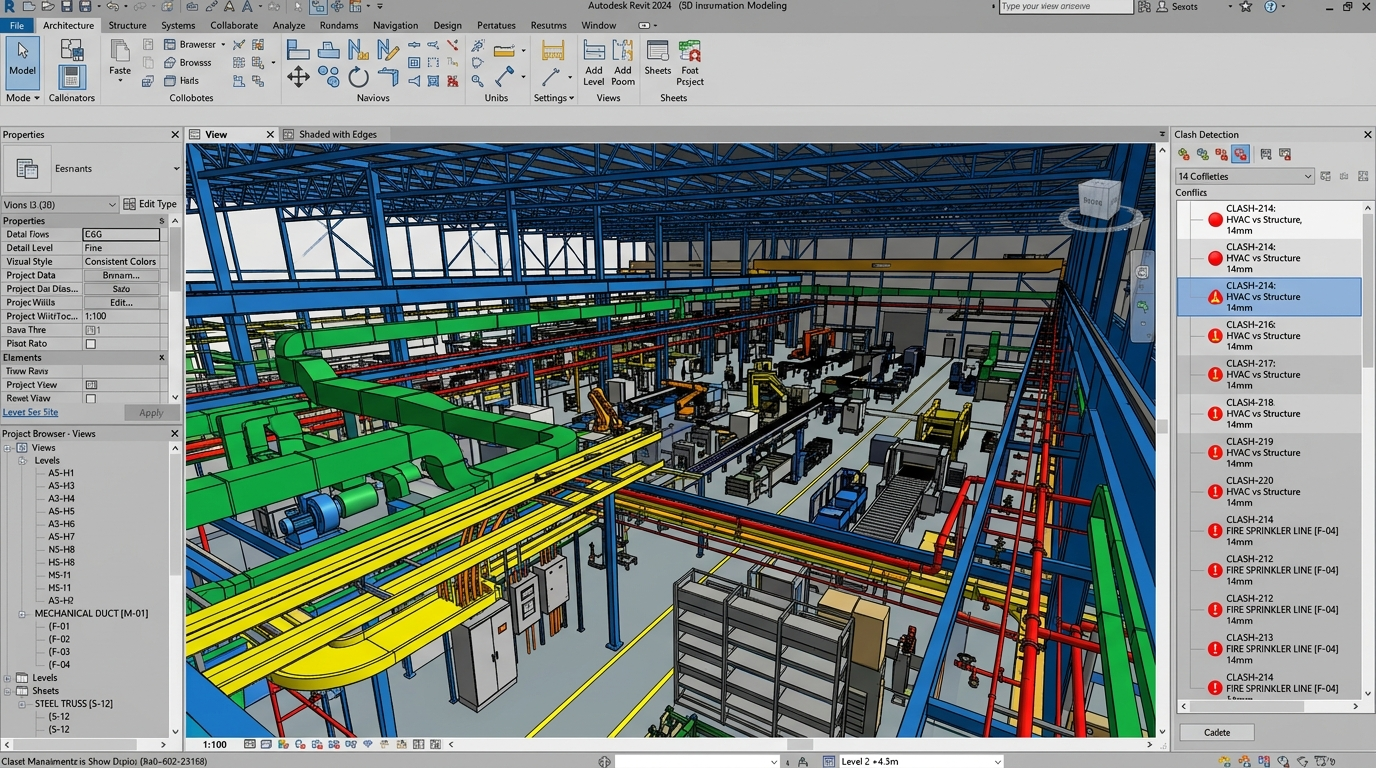
\includegraphics[width=186mm]{../../public/bim-model-3d.jpg}};
  \fill[TTCDeepNavy,opacity=.88] (0,0) rectangle (61,68);
  \fill[TTCDeepNavy,opacity=.24] (61,0) rectangle (86,68);
  \node[anchor=west,text width=48mm,align=left,text=white] at (8,44) {
    {\fontsize{7}{8}\selectfont\bfseries\color{TTCCyan} TTC DIGITAL THREAD}\\[1.4mm]
    {\fontsize{19}{21}\selectfont\bfseries DATA TO}\\[-.3mm]
    {\fontsize{19}{21}\selectfont\bfseries\color{TTCRed!85!white} DECISION}\\[1.8mm]
    {\fontsize{7}{8.5}\selectfont\color{white!82!gray}
    Một nguồn dữ liệu tin cậy cho thiết kế, công trường và đội vận hành.}
  };
  \node[rounded corners=2pt,fill=white,align=center,minimum width=27mm,
        minimum height=15mm] at (111,15) {
    {\fontsize{9}{10}\selectfont\bfseries\color{TTCBlue} DESIGN}\\[-.2mm]
    {\fontsize{5.8}{7}\selectfont LOD 400 • 5D}
  };
  \node[rounded corners=2pt,fill=TTCCyan,align=center,text=white,
        minimum width=27mm,minimum height=15mm] at (143,15) {
    {\fontsize{9}{10}\selectfont\bfseries BUILD}\\[-.2mm]
    {\fontsize{5.8}{7}\selectfont Clash • 4D}
  };
  \node[rounded corners=2pt,fill=TTCGold,align=center,text=white,
        minimum width=27mm,minimum height=15mm] at (172,15) {
    {\fontsize{9}{10}\selectfont\bfseries OPERATE}\\[-.2mm]
    {\fontsize{5.8}{7}\selectfont Twin • O\&M}
  };
\end{tikzpicture}

\vspace{3mm}

% THREE DECISION ENGINES
\noindent
\begin{tikzpicture}[x=1mm,y=1mm]
  \path[use as bounding box] (0,0) rectangle (186,62);
  \foreach \x/\c in {0/TTCRed,63/TTCCyan,126/TTCGold}{
    \fill[white,rounded corners=2pt] (\x,0) rectangle +(60,62);
    \draw[TTCBorder,rounded corners=2pt,line width=.6pt] (\x,0) rectangle +(60,62);
    \fill[\c,rounded corners=2pt] (\x,58) rectangle +(60,4);
  }
  \node[anchor=north west,text width=50mm] at (5,53) {
    {\fontsize{7}{8}\selectfont\bfseries\color{TTCRed} 01 / COORDINATE}\\[1mm]
    {\fontsize{11}{12}\selectfont\bfseries\color{TTCBlue} BIM 5D}\\[1.2mm]
    {\fontsize{6.8}{8.2}\selectfont\color{TTCTextDark}
    \textbf{Input:} Kiến trúc • Kết cấu • MEP\newline
    \textbf{Decision:} Clash-check và sequence\newline
    \textbf{Output:} Shop Drawing, BOQ, 4D plan}\\[1mm]
    {\fontsize{6.2}{7.3}\selectfont\bfseries\color{TTCTextMuted} TEKLA • REVIT • NAVISWORKS}
  };
  \node[anchor=north west,text width=50mm] at (68,53) {
    {\fontsize{7}{8}\selectfont\bfseries\color{TTCCyan} 02 / OPTIMIZE}\\[1mm]
    {\fontsize{11}{12}\selectfont\bfseries\color{TTCBlue} AI STRUCTURE}\\[1.2mm]
    {\fontsize{6.8}{8.2}\selectfont\color{TTCTextDark}
    \textbf{Input:} Tải trọng • nhịp • nội lực\newline
    \textbf{Decision:} Lặp phương án tiết diện\newline
    \textbf{Output:} Dầm Tapered tối ưu 10--15\%}\\[1mm]
    {\fontsize{6.2}{7.3}\selectfont\bfseries\color{TTCTextMuted} AISC 360 • TCVN • AIDC R\&D}
  };
  \node[anchor=north west,text width=50mm] at (131,53) {
    {\fontsize{7}{8}\selectfont\bfseries\color{TTCGold} 03 / OPERATE}\\[1mm]
    {\fontsize{11}{12}\selectfont\bfseries\color{TTCBlue} DIGITAL TWIN}\\[1.2mm]
    {\fontsize{6.8}{8.2}\selectfont\color{TTCTextDark}
    \textbf{Input:} As-built • tài sản • IoT\newline
    \textbf{Decision:} Bảo trì theo trạng thái\newline
    \textbf{Output:} O\&M có truy vết 30+ năm}\\[1mm]
    {\fontsize{6.2}{7.3}\selectfont\bfseries\color{TTCTextMuted} CDE • BMS • SCADA READY}
  };
\end{tikzpicture}

\vspace{3mm}

% DIGITAL THREAD FLOW
\noindent
\begin{tikzpicture}[x=1mm,y=1mm]
  \path[use as bounding box] (0,0) rectangle (186,42);
  \fill[TTCLightBlue,rounded corners=3pt] (0,0) rectangle (186,42);
  \draw[TTCBorder,rounded corners=3pt,line width=.6pt] (0,0) rectangle (186,42);
  \node[anchor=west,text=TTCBlue,font=\fontsize{8}{9.5}\selectfont\bfseries] at (7,34)
    {\faDatabase\quad DIGITAL THREAD — DỮ LIỆU KHÔNG BỊ ĐỨT GÃY};
  \foreach \x/\n/\t in {24/01/MODEL,70/02/APPROVE,116/03/BUILD,162/04/OPERATE}{
    \fill[white] (\x,17) circle (5);
    \draw[TTCBlue,line width=.8pt] (\x,17) circle (5);
    \node[text=TTCRed,font=\fontsize{6.4}{7}\selectfont\bfseries] at (\x,17) {\n};
    \node[anchor=north,align=center,text width=34mm] at (\x,9) {
      {\fontsize{6.7}{8}\selectfont\bfseries\color{TTCBlue} \t}
    };
  }
  \draw[-{Stealth[length=2.2mm]},TTCBlue!45!white,line width=.9pt] (30,17) -- (64,17);
  \draw[-{Stealth[length=2.2mm]},TTCBlue!45!white,line width=.9pt] (76,17) -- (110,17);
  \draw[-{Stealth[length=2.2mm]},TTCBlue!45!white,line width=.9pt] (122,17) -- (156,17);
\end{tikzpicture}

\vspace{3mm}

% KPI MEMORY STRIP
\noindent
\begin{tikzpicture}[x=1mm,y=1mm]
  \path[use as bounding box] (0,0) rectangle (186,29);
  \fill[TTCDeepNavy,rounded corners=3pt] (0,0) rectangle (186,29);
  \foreach \x in {46.5,93,139.5}{\draw[white!35!gray] (\x,6) -- (\x,23);}
  \node[align=center,text=white] at (23.25,15) {{\fontsize{9}{10}\selectfont\bfseries\color{TTCRed} LOD 400}\\[-.3mm]{\fontsize{6.2}{7.4}\selectfont Fabrication Detail}};
  \node[align=center,text=white] at (69.75,15) {{\fontsize{9}{10}\selectfont\bfseries\color{TTCCyan} 10--15\%}\\[-.3mm]{\fontsize{6.2}{7.4}\selectfont Steel Optimization}};
  \node[align=center,text=white] at (116.25,15) {{\fontsize{9}{10}\selectfont\bfseries CLASH-FREE}\\[-.3mm]{\fontsize{6.2}{7.4}\selectfont Coordinated Model}};
  \node[align=center,text=white] at (162.75,15) {{\fontsize{9}{10}\selectfont\bfseries\color{TTCGold} 30+ NĂM}\\[-.3mm]{\fontsize{6.2}{7.4}\selectfont Digital O\&M}};
\end{tikzpicture}
\end{minipage}
\newpage

% ============================================================
% TRANG 16: ESG BUSINESS CASE — GREEN FACTORY
% ============================================================
\pageheaderbar{CÔNG TRÌNH XANH ESG \& MÁI SOLAR-READY}{Trang 16}
\pagefooterbar{Trang 16}

\begin{tikzpicture}[remember picture, overlay]
  \fill[TTCLightBlue]
    ([xshift=125mm,yshift=-30mm]current page.north west) --
    ([xshift=210mm,yshift=-30mm]current page.north west) --
    ([xshift=210mm,yshift=-112mm]current page.north west) -- cycle;
  \node[opacity=.03,text=TTCBlue,font=\fontsize{64}{66}\selectfont\bfseries,
        rotate=90] at ([xshift=-11mm,yshift=2mm]current page.east) {ESG};
  % Solar roof rhythm at the bottom
  \begin{scope}[shift={(current page.south west)},x=1mm,y=1mm,opacity=.43]
    \draw[TTCBlue!17!white,line width=.7pt] (14,13) -- (196,13);
    \foreach \x in {18,48,78,108,138,168}{
      \fill[TTCBlue!3!white] (\x,14) -- ++(24,0) -- ++(-5,17) -- ++(-24,0) -- cycle;
      \draw[TTCBlue!16!white] (\x,14) -- ++(24,0) -- ++(-5,17) -- ++(-24,0) -- cycle;
      \draw[TTCBlue!11!white] (\x+4,14) -- (\x-1,31);
      \draw[TTCBlue!11!white] (\x+12,14) -- (\x+7,31);
    }
    \draw[TTCCyan!22!white,line width=.8pt] (24,38) arc[start angle=210,end angle=330,radius=10mm];
    \draw[TTCRed!18!white,line width=.7pt] (24,38) -- (24,45);
  \end{scope}
\end{tikzpicture}

\begin{minipage}[t][246mm]{\textwidth}
\secbrand{Nhà Máy Xanh Được Thiết Kế Như Một Bài Toán Kinh Doanh}{Solar-Ready, Low-Energy Envelope, Water Circularity \& Green Certification}

{\fontsize{15}{17}\selectfont\bfseries\color{TTCBlue}
GIẢM OPEX • SẴN SÀNG CARBON • TĂNG GIÁ TRỊ TÀI SẢN\par}
\vspace{1mm}
{\fontsize{7.5}{9}\selectfont\color{TTCTextMuted}
ESG được tích hợp từ kết cấu và vỏ bao che — không phải bổ sung tốn kém sau khi nhà máy đã vận hành.\par}
\vspace{3mm}

% HERO — GREEN FACTORY
\noindent
\begin{tikzpicture}[x=1mm,y=1mm]
  \path[use as bounding box] (0,0) rectangle (186,70);
  \clip[rounded corners=3pt] (0,0) rectangle (186,70);
  \node[anchor=center,inner sep=0pt] at (93,35)
    {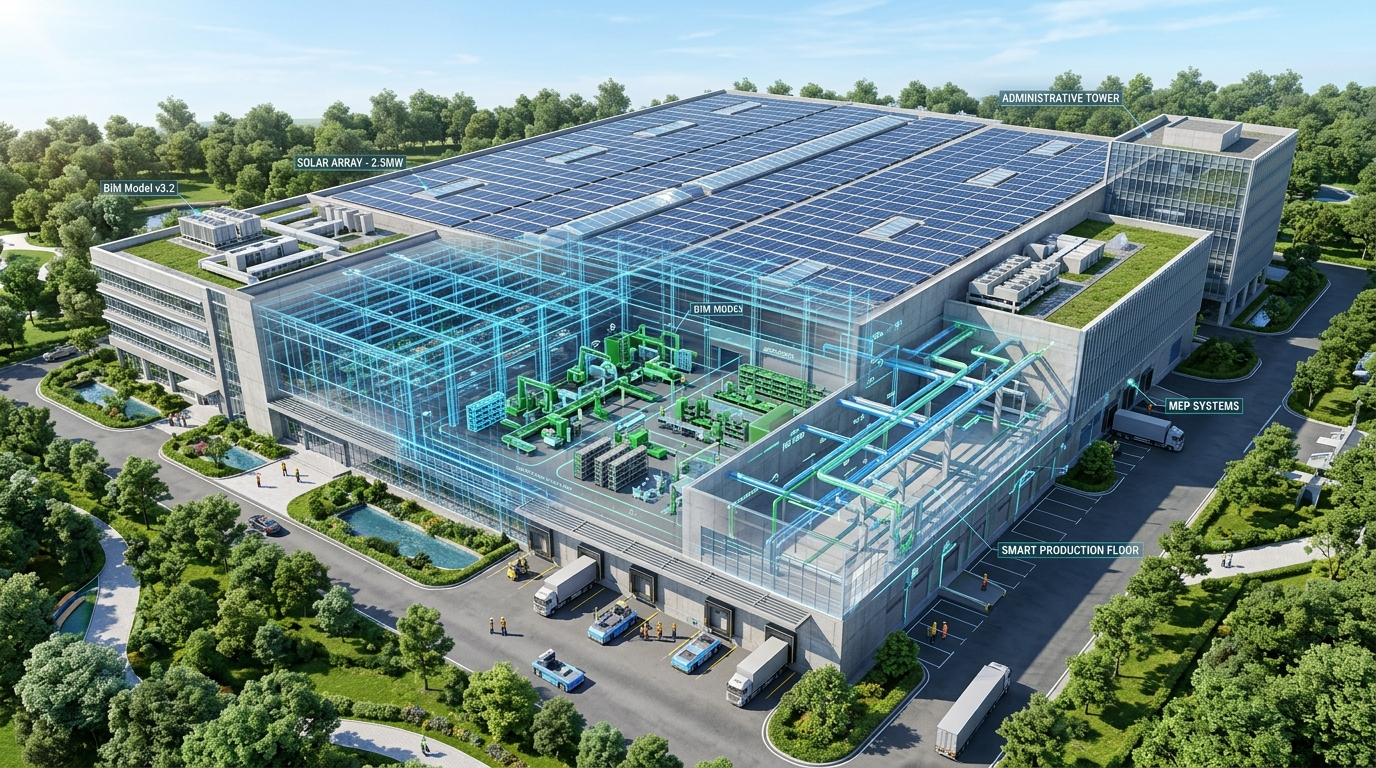
\includegraphics[width=186mm]{../../public/bim-esg-factory-3d.jpg}};
  \fill[TTCDeepNavy,opacity=.84] (0,0) rectangle (61,70);
  \fill[TTCDeepNavy,opacity=.22] (61,0) rectangle (87,70);
  \node[anchor=west,text width=48mm,align=left,text=white] at (8,46) {
    {\fontsize{7}{8}\selectfont\bfseries\color{TTCCyan} ESG-BY-DESIGN}\\[1.3mm]
    {\fontsize{17}{19}\selectfont\bfseries NET-ZERO}\\[-.2mm]
    {\fontsize{17}{19}\selectfont\bfseries\color{TTCRed!85!white} READY}\\[1.8mm]
    {\fontsize{7}{8.5}\selectfont\color{white!82!gray}
    Kết cấu, năng lượng, nước và vận hành được chuẩn bị trong cùng một mô hình.}
  };
  \node[rounded corners=2pt,fill=white,align=center,minimum width=31mm,
        minimum height=15mm] at (121,15) {
    {\fontsize{10}{11}\selectfont\bfseries\color{TTCRed} 1--5 MWp}\\[-.2mm]
    {\fontsize{5.8}{7}\selectfont\color{TTCBlue} SOLAR-READY}
  };
  \node[rounded corners=2pt,fill=TTCCyan,align=center,text=white,
        minimum width=31mm,minimum height=15mm] at (155,15) {
    {\fontsize{10}{11}\selectfont\bfseries -20\%}\\[-.2mm]
    {\fontsize{5.8}{7}\selectfont HVAC ENERGY}
  };
\end{tikzpicture}

\vspace{3mm}

% FOUR ESG LEVERS
\noindent
\begin{tikzpicture}[x=1mm,y=1mm]
  \path[use as bounding box] (0,0) rectangle (186,51);
  \foreach \x/\c in {0/TTCRed,47.5/TTCCyan,95/TTCBlue,142.5/TTCGold}{
    \fill[white,rounded corners=2pt] (\x,0) rectangle +(43.5,51);
    \draw[TTCBorder,rounded corners=2pt,line width=.6pt] (\x,0) rectangle +(43.5,51);
    \fill[\c,rounded corners=2pt] (\x,47) rectangle +(43.5,4);
  }
  \node[anchor=north west,text width=35mm] at (4,43) {
    {\fontsize{7}{8}\selectfont\bfseries\color{TTCRed} 01 / ENERGY}\\[1mm]
    {\fontsize{8.5}{10}\selectfont\bfseries\color{TTCBlue} SOLAR-READY}\\[1mm]
    {\fontsize{6.5}{7.8}\selectfont\color{TTCTextDark}
    Dự phòng tải mái, xà gồ và Seamlock cho hệ pin 1--5MWp.}
  };
  \node[anchor=north west,text width=35mm] at (51.5,43) {
    {\fontsize{7}{8}\selectfont\bfseries\color{TTCCyan} 02 / ENVELOPE}\\[1mm]
    {\fontsize{8.5}{10}\selectfont\bfseries\color{TTCBlue} COOL ROOF}\\[1mm]
    {\fontsize{6.5}{7.8}\selectfont\color{TTCTextDark}
    Panel PIR/Rockwool và mái phản xạ nhiệt giảm tải HVAC.}
  };
  \node[anchor=north west,text width=35mm] at (99,43) {
    {\fontsize{7}{8}\selectfont\bfseries\color{TTCBlue} 03 / WATER}\\[1mm]
    {\fontsize{8.5}{10}\selectfont\bfseries\color{TTCBlue} CIRCULARITY}\\[1mm]
    {\fontsize{6.5}{7.8}\selectfont\color{TTCTextDark}
    Nước thải Cột A, thu nước mưa và tái sử dụng cho cảnh quan.}
  };
  \node[anchor=north west,text width=35mm] at (146.5,43) {
    {\fontsize{7}{8}\selectfont\bfseries\color{TTCGold} 04 / STANDARD}\\[1mm]
    {\fontsize{8.5}{10}\selectfont\bfseries\color{TTCBlue} LEED / LOTUS}\\[1mm]
    {\fontsize{6.5}{7.8}\selectfont\color{TTCTextDark}
    Mô phỏng năng lượng, vật liệu Low-VOC và hồ sơ chứng nhận.}
  };
\end{tikzpicture}

\vspace{3mm}

% ESG BUSINESS CASE
\noindent
\begin{tikzpicture}[x=1mm,y=1mm]
  \path[use as bounding box] (0,0) rectangle (186,47);
  \fill[TTCLightBlue,rounded corners=3pt] (0,0) rectangle (186,47);
  \draw[TTCBorder,rounded corners=3pt,line width=.6pt] (0,0) rectangle (186,47);
  \node[anchor=west,text=TTCBlue,font=\fontsize{8}{9.5}\selectfont\bfseries] at (7,39)
    {\faGlobeAmericas\quad BUSINESS CASE CHO CHỦ ĐẦU TƯ FDI};
  \foreach \x in {62,124}{\draw[TTCBorder] (\x,6) -- (\x,31);}
  \node[align=left,text width=50mm,anchor=north west] at (6,30) {
    {\fontsize{8}{9.5}\selectfont\bfseries\color{TTCRed} GREEN FINANCE}\\[.7mm]
    {\fontsize{6.5}{7.8}\selectfont\color{TTCTextDark}
    Tăng khả năng tiếp cận nguồn vốn xanh và tiêu chí chuỗi cung ứng quốc tế.}
  };
  \node[align=left,text width=50mm,anchor=north west] at (68,30) {
    {\fontsize{8}{9.5}\selectfont\bfseries\color{TTCCyan} CARBON READY}\\[.7mm]
    {\fontsize{6.5}{7.8}\selectfont\color{TTCTextDark}
    Chuẩn bị dữ liệu năng lượng và vật liệu cho CBAM, I-REC và Net-Zero roadmap.}
  };
  \node[align=left,text width=50mm,anchor=north west] at (130,30) {
    {\fontsize{8}{9.5}\selectfont\bfseries\color{TTCGold} LOWER OPEX}\\[.7mm]
    {\fontsize{6.5}{7.8}\selectfont\color{TTCTextDark}
    Giảm điện HVAC, tối ưu nước vận hành và nâng giá trị khai thác tài sản.}
  };
\end{tikzpicture}

\vspace{3mm}

% KPI MEMORY STRIP
\noindent
\begin{tikzpicture}[x=1mm,y=1mm]
  \path[use as bounding box] (0,0) rectangle (186,29);
  \fill[TTCDeepNavy,rounded corners=3pt] (0,0) rectangle (186,29);
  \foreach \x in {46.5,93,139.5}{\draw[white!35!gray] (\x,6) -- (\x,23);}
  \node[align=center,text=white] at (23.25,15) {{\fontsize{9}{10}\selectfont\bfseries\color{TTCRed} 1--5 MWp}\\[-.3mm]{\fontsize{6.2}{7.4}\selectfont Solar-Ready Roof}};
  \node[align=center,text=white] at (69.75,15) {{\fontsize{9}{10}\selectfont\bfseries\color{TTCCyan} -20\% ĐIỆN}\\[-.3mm]{\fontsize{6.2}{7.4}\selectfont HVAC Energy}};
  \node[align=center,text=white] at (116.25,15) {{\fontsize{9}{10}\selectfont\bfseries CỘT A}\\[-.3mm]{\fontsize{6.2}{7.4}\selectfont Water Treatment}};
  \node[align=center,text=white] at (162.75,15) {{\fontsize{9}{10}\selectfont\bfseries\color{TTCGold} LEED READY}\\[-.3mm]{\fontsize{6.2}{7.4}\selectfont Green Certification}};
\end{tikzpicture}
\end{minipage}
\newpage

% ============================================================
% TRANG 17: DIGITAL SITE CONTROL CENTER
% ============================================================
\pageheaderbar{TRUNG TÂM ĐIỀU HÀNH CÔNG TRƯỜNG SỐ}{Trang 17}
\pagefooterbar{Trang 17}

\begin{tikzpicture}[remember picture, overlay]
  \fill[TTCLightBlue]
    ([xshift=131mm,yshift=-30mm]current page.north west) --
    ([xshift=210mm,yshift=-30mm]current page.north west) --
    ([xshift=210mm,yshift=-115mm]current page.north west) -- cycle;
  % Data pulse background — deliberately different from the previous pages
  \begin{scope}[shift={(current page.south west)},x=1mm,y=1mm,opacity=.45]
    \draw[TTCBlue!18!white,line width=.8pt] (13,17) -- (197,17);
    \draw[TTCBlue!15!white] (20,17) -- (38,35) -- (62,25) -- (86,45) --
      (112,29) -- (139,42) -- (164,26) -- (191,38);
    \foreach \x/\y in {20/17,38/35,62/25,86/45,112/29,139/42,164/26,191/38}{
      \fill[TTCCyan!20!white] (\x,\y) circle (1.7);
      \draw[TTCBlue!20!white] (\x,\y) circle (3.1);
    }
  \end{scope}
\end{tikzpicture}

\begin{minipage}[t][246mm]{\textwidth}
\secbrand{Trung Tâm Điều Hành Công Trường Số}{Dữ liệu tập trung • Cảnh báo tức thời • Hồ sơ truy xuất được}

{\fontsize{15}{17}\selectfont\bfseries\color{TTCBlue}
MỘT CÔNG TRƯỜNG • BA NGUỒN DỮ LIỆU • MỘT ĐẦU MỐI ĐIỀU HÀNH\par}
\vspace{1mm}
{\fontsize{7.5}{9}\selectfont\color{TTCTextMuted}
Tập trung dữ liệu con người, an toàn và hồ sơ thi công để Chỉ huy trưởng xử lý đúng việc, đúng thời điểm.\par}
\vspace{3mm}

% CONTROL CENTER DASHBOARD
\noindent
\begin{tikzpicture}[x=1mm,y=1mm]
  \path[use as bounding box] (0,0) rectangle (186,101);
  \fill[TTCDeepNavy,rounded corners=3pt] (0,0) rectangle (186,101);
  \draw[TTCCyan!65!white,rounded corners=3pt,line width=.8pt] (0,0) rectangle (186,101);

  \node[anchor=west,text=white,font=\fontsize{8}{9.5}\selectfont\bfseries] at (8,93)
    {\faDesktop\quad TRUNG TÂM ĐIỀU HÀNH};
  \node[anchor=east,text=TTCCyan,font=\fontsize{6.3}{7.5}\selectfont\bfseries] at (121,93)
    {DỮ LIỆU THẬT • HÀNH ĐỘNG CÓ LƯU VẾT};

  % Status row
  \foreach \x/\c in {8/TTCRed,47/TTCCyan,86/TTCGold}{
    \fill[white!7!TTCDeepNavy,rounded corners=2pt] (\x,63) rectangle +(34,21);
    \draw[\c!70!white,rounded corners=2pt,line width=.55pt] (\x,63) rectangle +(34,21);
  }
  \node[anchor=west,text=TTCRed,font=\fontsize{6.2}{7.3}\selectfont\bfseries] at (11,78) {KIỂM SOÁT RA VÀO};
  \node[anchor=west,text=white,font=\fontsize{9.2}{10.5}\selectfont\bfseries] at (11,70) {ĐÚNG NGƯỜI};
  \node[anchor=west,text=TTCCyan,font=\fontsize{6.2}{7.3}\selectfont\bfseries] at (50,78) {GIÁM SÁT AN TOÀN};
  \node[anchor=west,text=white,font=\fontsize{9.2}{10.5}\selectfont\bfseries] at (50,70) {ĐÚNG QUY TẮC};
  \node[anchor=west,text=TTCGold,font=\fontsize{6.2}{7.3}\selectfont\bfseries] at (89,78) {HỒ SƠ HIỆN TRƯỜNG};
  \node[anchor=west,text=white,font=\fontsize{9.2}{10.5}\selectfont\bfseries] at (89,70) {ĐÚNG PHIÊN BẢN};

  % Three real data streams
  \fill[white,rounded corners=2pt] (8,29) rectangle (40,55);
  \fill[white,rounded corners=2pt] (47,29) rectangle (79,55);
  \fill[white,rounded corners=2pt] (86,29) rectangle (118,55);
  \node[align=center,text width=27mm] at (24,42) {
    {\fontsize{7.5}{9}\selectfont\bfseries\color{TTCRed} NHÂN SỰ}\\[-.2mm]
    {\fontsize{6.2}{7.4}\selectfont\color{TTCTextMuted}FaceID • đào tạo\\chứng chỉ vào cổng}
  };
  \node[align=center,text width=27mm] at (63,42) {
    {\fontsize{7.5}{9}\selectfont\bfseries\color{TTCCyan} AN TOÀN}\\[-.2mm]
    {\fontsize{6.2}{7.4}\selectfont\color{TTCTextMuted}Camera AI • PPE\\vùng nguy hiểm}
  };
  \node[align=center,text width=27mm] at (102,42) {
    {\fontsize{7.5}{9}\selectfont\bfseries\color{TTCGold} HỒ SƠ}\\[-.2mm]
    {\fontsize{6.2}{7.4}\selectfont\color{TTCTextMuted}CDE • ITP • RFI\\nhật ký số}
  };
  \draw[-{Stealth[length=2mm]},TTCCyan,line width=.8pt] (40.5,42) -- (46,42);
  \draw[-{Stealth[length=2mm]},TTCCyan,line width=.8pt] (79.5,42) -- (85,42);

  % Decision layer
  \fill[TTCCyan!12!TTCDeepNavy,rounded corners=2pt] (8,7) rectangle (118,21);
  \node[anchor=west,text=TTCCyan,font=\fontsize{6}{7}\selectfont\bfseries] at (12,14)
    {LỚP ĐIỀU HÀNH};
  \node[anchor=west,text=white,font=\fontsize{7}{8.5}\selectfont\bfseries] at (40,14)
    {Cảnh báo → Phân công → Phê duyệt → Lưu bằng chứng};

  % Ảnh hiện trường có vùng chú thích riêng, không đặt chữ lên ảnh
  \begin{scope}
    \clip[rounded corners=2pt] (126,16) rectangle (179,86);
    \node[anchor=center,inner sep=0pt] at (152.5,51)
      {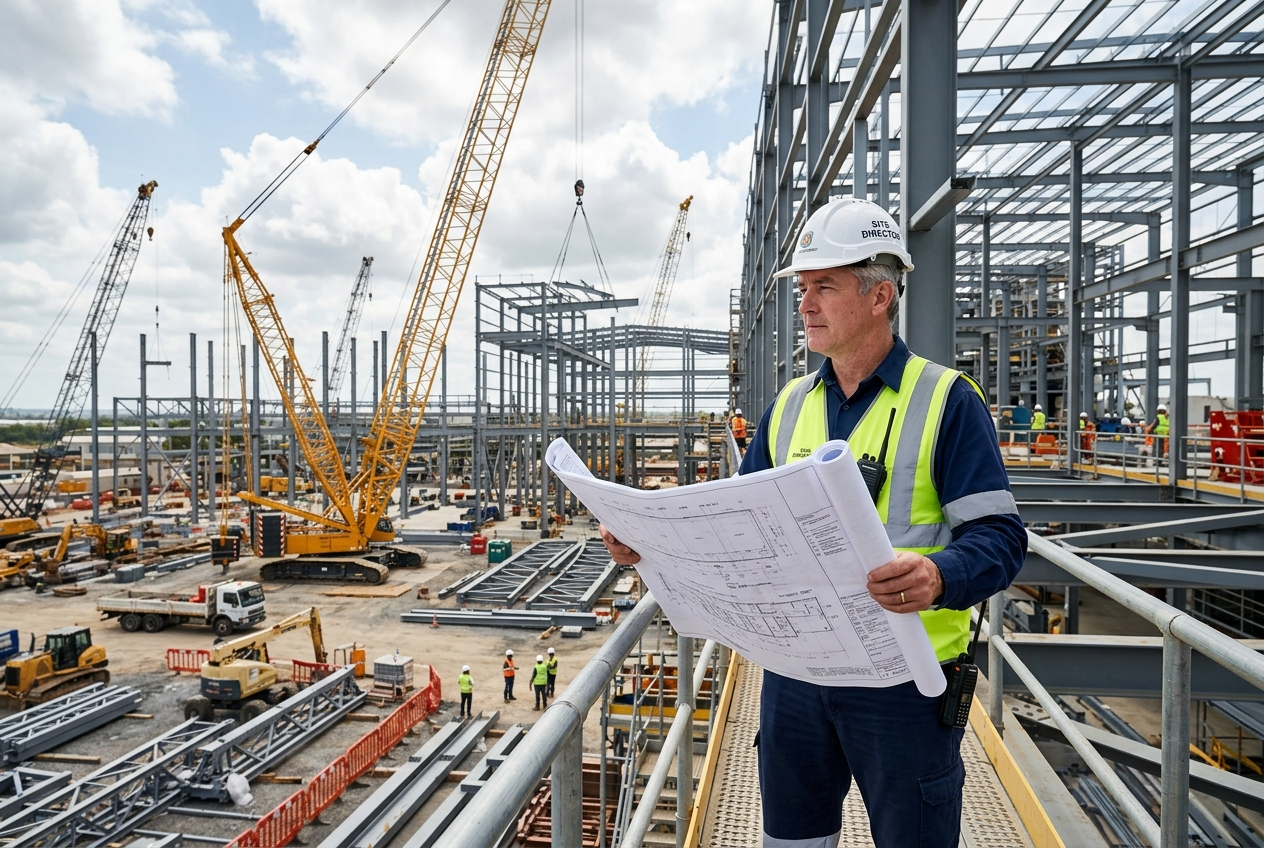
\includegraphics[height=70mm]{../../public/c_level_site_inspection.jpg}};
  \end{scope}
  \draw[white!45!gray,rounded corners=2pt,line width=.6pt] (126,16) rectangle (179,86);
  \fill[TTCBlue] (126,7) rectangle (179,15);
  \node[text=white,font=\fontsize{6.4}{7.5}\selectfont\bfseries] at (152.5,11)
    {HÌNH ẢNH HIỆN TRƯỜNG};
\end{tikzpicture}

\vspace{3mm}

% OWNER VIEW — THREE OUTCOMES
\noindent
\begin{tikzpicture}[x=1mm,y=1mm]
  \path[use as bounding box] (0,0) rectangle (186,49);
  \fill[white,rounded corners=3pt] (0,0) rectangle (186,49);
  \draw[TTCBorder,rounded corners=3pt,line width=.6pt] (0,0) rectangle (186,49);
  \node[anchor=west,text=TTCBlue,font=\fontsize{8}{9.5}\selectfont\bfseries] at (7,41)
    {\faMobile*\quad THÔNG TIN ĐỦ ĐỂ RA QUYẾT ĐỊNH};
  \foreach \x in {62,124}{\draw[TTCBorder] (\x,7) -- (\x,33);}
  \node[anchor=north west,text width=50mm] at (6,31) {
    {\fontsize{8}{9.5}\selectfont\bfseries\color{TTCRed} QUÂN SỐ SẴN SÀNG}\\[.7mm]
    {\fontsize{6.6}{8}\selectfont\color{TTCTextDark}
    Biết ai đang ở công trường và điều kiện vào cổng của từng người.}
  };
  \node[anchor=north west,text width=50mm] at (68,31) {
    {\fontsize{8}{9.5}\selectfont\bfseries\color{TTCCyan} AN TOÀN HIỂN THỊ}\\[.7mm]
    {\fontsize{6.6}{8}\selectfont\color{TTCTextDark}
    Cảnh báo vi phạm PPE và xâm nhập vùng nguy hiểm để xử lý tức thời.}
  };
  \node[anchor=north west,text width=50mm] at (130,31) {
    {\fontsize{8}{9.5}\selectfont\bfseries\color{TTCGold} HỒ SƠ ĐẦY ĐỦ}\\[.7mm]
    {\fontsize{6.6}{8}\selectfont\color{TTCTextDark}
    Nhật ký, RFI và hồ sơ ITP có thời gian, người duyệt và bằng chứng.}
  };
\end{tikzpicture}

\vspace{3mm}

% ACTION LOOP — NO KPI GRID
\noindent
\begin{tikzpicture}[x=1mm,y=1mm]
  \path[use as bounding box] (0,0) rectangle (186,43);
  \fill[TTCLightBlue,rounded corners=3pt] (0,0) rectangle (186,43);
  \draw[TTCBorder,rounded corners=3pt,line width=.6pt] (0,0) rectangle (186,43);
  \node[anchor=west,text=TTCBlue,font=\fontsize{8}{9.5}\selectfont\bfseries] at (7,35)
    {\faCheckCircle\quad VÒNG LẶP HÀNH ĐỘNG TRONG NGÀY};
  \foreach \x/\n/\t in {23/01/GHI NHẬN,69/02/CẢNH BÁO,115/03/XỬ LÝ,161/04/LƯU VẾT}{
    \fill[white] (\x,17) circle (5);
    \draw[TTCBlue,line width=.8pt] (\x,17) circle (5);
    \node[text=TTCRed,font=\fontsize{6.3}{7}\selectfont\bfseries] at (\x,17) {\n};
    \node[anchor=north,align=center,text width=34mm] at (\x,9)
      {{\fontsize{6.7}{8}\selectfont\bfseries\color{TTCBlue} \t}};
  }
  \draw[-{Stealth[length=2mm]},TTCBlue!45!white,line width=.9pt] (29,17) -- (63,17);
  \draw[-{Stealth[length=2mm]},TTCBlue!45!white,line width=.9pt] (75,17) -- (109,17);
  \draw[-{Stealth[length=2mm]},TTCBlue!45!white,line width=.9pt] (121,17) -- (155,17);
\end{tikzpicture}
\end{minipage}
\newpage

% ============================================================
% TRANG 18: QUALITY PASSPORT & RELEASE GATES
% ============================================================
\pageheaderbar{HỆ THỐNG QUẢN LÝ CHẤT LƯỢNG QA/QC}{Trang 18}
\pagefooterbar{Trang 18}

\begin{tikzpicture}[remember picture, overlay]
  \fill[TTCLightBlue]
    ([xshift=121mm,yshift=-31mm]current page.north west) --
    ([xshift=210mm,yshift=-31mm]current page.north west) --
    ([xshift=210mm,yshift=-118mm]current page.north west) -- cycle;
  % document trace lines at the bottom
  \begin{scope}[shift={(current page.south west)},x=1mm,y=1mm,opacity=.43]
    \draw[TTCBlue!17!white,line width=.7pt] (14,15) -- (196,15);
    \foreach \x in {18,56,94,132,170}{
      \draw[TTCBlue!15!white,rounded corners=1pt] (\x,15) rectangle +(25,28);
      \draw[TTCRed!14!white] (\x+5,35) -- (\x+20,35);
      \draw[TTCBlue!11!white] (\x+5,29) -- (\x+20,29);
      \draw[TTCBlue!11!white] (\x+5,23) -- (\x+16,23);
    }
  \end{scope}
\end{tikzpicture}

\begin{minipage}[t][246mm]{\textwidth}
\secbrand{Hộ Chiếu Chất Lượng Cho Từng Gói Công Việc}{Kiểm soát ITP bốn cấp • Đủ bằng chứng mới chuyển bước}

{\fontsize{15}{17}\selectfont\bfseries\color{TTCBlue}
CHỈ CHUYỂN BƯỚC KHI ĐÃ CÓ ĐỦ BẰNG CHỨNG\par}
\vspace{1mm}
{\fontsize{7.5}{9}\selectfont\color{TTCTextMuted}
Mỗi vật liệu, mối hàn và hạng mục được kiểm tra, ký xác nhận và lưu vết trước khi phát hành cho bước tiếp theo.\par}
\vspace{3mm}

% QUALITY GATES + PASSPORT
\noindent
\begin{tikzpicture}[x=1mm,y=1mm]
  \path[use as bounding box] (0,0) rectangle (186,122);

  % Left release ladder
  \fill[TTCDeepNavy,rounded corners=3pt] (0,0) rectangle (57,122);
  \node[anchor=west,text=TTCCyan,font=\fontsize{7}{8}\selectfont\bfseries] at (6,113)
    {4 CẤP KIỂM SOÁT};
  \node[anchor=west,text=white,font=\fontsize{11}{12}\selectfont\bfseries] at (6,106.5)
    {CỔNG ITP};

  \foreach \y/\n/\c in {78/01/TTCRed,52/02/TTCBlue,26/03/TTCCyan,0/04/TTCGold}{
    \fill[white,rounded corners=2pt] (6,\y+6) rectangle (51,\y+25);
    \draw[\c,rounded corners=2pt,line width=.7pt] (6,\y+6) rectangle (51,\y+25);
    \fill[\c] (6,\y+6) rectangle (13,\y+25);
    \node[text=white,font=\fontsize{6.5}{7}\selectfont\bfseries] at (9.5,\y+15.5) {\n};
  }
  \node[anchor=west,text width=33mm] at (16,93.5) {
    {\fontsize{7.2}{8.5}\selectfont\bfseries\color{TTCRed} TỔ ĐỘI TỰ KIỂM}\\[-.2mm]
    {\fontsize{6.2}{7.4}\selectfont\color{TTCTextMuted}Phiếu tự kiểm nội bộ}
  };
  \node[anchor=west,text width=33mm] at (16,67.5) {
    {\fontsize{7.2}{8.5}\selectfont\bfseries\color{TTCBlue} KỸ SƯ HIỆN TRƯỜNG}\\[-.2mm]
    {\fontsize{6.2}{7.4}\selectfont\color{TTCTextMuted}Bản vẽ thi công • ITP}
  };
  \node[anchor=west,text width=33mm] at (16,41.5) {
    {\fontsize{7.2}{8.5}\selectfont\bfseries\color{TTCCyan} QA/QC ĐỘC LẬP}\\[-.2mm]
    {\fontsize{6.2}{7.4}\selectfont\color{TTCTextMuted}Biên bản NDT • kết quả thử}
  };
  \node[anchor=west,text width=33mm] at (16,15.5) {
    {\fontsize{7.2}{8.5}\selectfont\bfseries\color{TTCGold} TVGS / CHỦ ĐẦU TƯ}\\[-.2mm]
    {\fontsize{6.2}{7.4}\selectfont\color{TTCTextMuted}Chấp thuận cuối}
  };
  \draw[-{Stealth[length=2mm]},white!55!gray,line width=.8pt] (28.5,83) -- (28.5,78);
  \draw[-{Stealth[length=2mm]},white!55!gray,line width=.8pt] (28.5,57) -- (28.5,52);
  \draw[-{Stealth[length=2mm]},white!55!gray,line width=.8pt] (28.5,31) -- (28.5,26);

  % Right quality passport
  \fill[white,rounded corners=3pt] (62,0) rectangle (186,122);
  \draw[TTCBorder,rounded corners=3pt,line width=.7pt] (62,0) rectangle (186,122);
  \fill[TTCLightBlue,rounded corners=3pt] (62,101) rectangle (186,122);
  \node[anchor=west,text=TTCBlue,font=\fontsize{10}{11.5}\selectfont\bfseries] at (68,113)
    {\faClipboardCheck\quad HỒ SƠ CHẤT LƯỢNG HẠNG MỤC};
  \node[anchor=east,text=TTCTextMuted,font=\fontsize{6}{7}\selectfont\bfseries] at (180,113)
    {MÃ GÓI VIỆC / HỒ SƠ TRUY XUẤT};

  \foreach \y/\n/\c in {78/01/TTCRed,55/02/TTCBlue,32/03/TTCCyan,9/04/TTCGold}{
    \fill[\c!6!white,rounded corners=1.5pt] (68,\y) rectangle (180,\y+18);
    \node[anchor=west,text=\c,font=\fontsize{7}{8}\selectfont\bfseries] at (72,\y+12) {\n};
    \fill[\c] (165,\y+5) circle (2.3);
    \node[text=white,font=\fontsize{5}{5.5}\selectfont\bfseries] at (165,\y+5) {\faCheck};
    \node[anchor=west,text=TTCTextMuted,font=\fontsize{6.1}{7.2}\selectfont\bfseries] at (170,\y+5) {ĐẠT};
  }
  \node[anchor=west,text=TTCBlue,font=\fontsize{7.4}{8.7}\selectfont\bfseries] at (81,90) {NGUỒN GỐC VẬT LIỆU};
  \node[anchor=west,text=TTCTextDark,font=\fontsize{6.3}{7.5}\selectfont] at (81,84) {CO/CQ • số lô • chứng chỉ xuất xưởng • kiểm tra đầu vào};
  \node[anchor=west,text=TTCBlue,font=\fontsize{7.4}{8.7}\selectfont\bfseries] at (81,67) {KIỂM SOÁT HÀN};
  \node[anchor=west,text=TTCTextDark,font=\fontsize{6.3}{7.5}\selectfont] at (81,61) {WPS/PQR • mã thợ hàn • AWS D1.1 • sơ đồ mối hàn};
  \node[anchor=west,text=TTCBlue,font=\fontsize{7.4}{8.7}\selectfont\bfseries] at (81,44) {BẰNG CHỨNG KIỂM TRA};
  \node[anchor=west,text=TTCTextDark,font=\fontsize{6.3}{7.5}\selectfont] at (81,38) {VT • UT • MT/PT • biên bản kiểm tra độc lập};
  \node[anchor=west,text=TTCBlue,font=\fontsize{7.4}{8.7}\selectfont\bfseries] at (81,21) {HỒ SƠ HOÀN CÔNG};
  \node[anchor=west,text=TTCTextDark,font=\fontsize{6.3}{7.5}\selectfont] at (81,15) {ITP đã ký • NCR đã đóng • bản vẽ hoàn công • lưu CDE};
\end{tikzpicture}

\vspace{3mm}

% NDT TOOLBOX
\noindent
\begin{tikzpicture}[x=1mm,y=1mm]
  \path[use as bounding box] (0,0) rectangle (186,46);
  \fill[TTCLightBlue,rounded corners=3pt] (0,0) rectangle (186,46);
  \draw[TTCBorder,rounded corners=3pt,line width=.6pt] (0,0) rectangle (186,46);
  \node[anchor=west,text=TTCBlue,font=\fontsize{8}{9.5}\selectfont\bfseries] at (7,38)
    {\faCheckDouble\quad PHƯƠNG PHÁP KIỂM TRA NDT};
  \foreach \x in {46.5,93,139.5}{\draw[TTCBorder] (\x,6) -- (\x,31);}
  \node[align=center,text width=38mm] at (23.25,18) {
    {\fontsize{9}{10}\selectfont\bfseries\color{TTCRed} VT}\\[-.2mm]
    {\fontsize{6.1}{7.3}\selectfont Ngoại quan • kích thước • bề mặt}
  };
  \node[align=center,text width=38mm] at (69.75,18) {
    {\fontsize{9}{10}\selectfont\bfseries\color{TTCCyan} UT}\\[-.2mm]
    {\fontsize{6.3}{7.5}\selectfont Siêu âm kiểm tra mối hàn}
  };
  \node[align=center,text width=38mm] at (116.25,18) {
    {\fontsize{9}{10}\selectfont\bfseries\color{TTCBlue} MT / PT}\\[-.2mm]
    {\fontsize{6.3}{7.5}\selectfont Kiểm tra nứt bề mặt và mối góc}
  };
  \node[align=center,text width=38mm] at (162.75,18) {
    {\fontsize{9}{10}\selectfont\bfseries\color{TTCGold} LAS-XD}\\[-.2mm]
    {\fontsize{6.3}{7.5}\selectfont Kiểm chứng tại phòng thí nghiệm}
  };
\end{tikzpicture}

\vspace{3mm}

% RELEASE OUTCOME
\noindent
\begin{tikzpicture}[x=1mm,y=1mm]
  \path[use as bounding box] (0,0) rectangle (186,30);
  \fill[TTCDeepNavy,rounded corners=3pt] (0,0) rectangle (186,30);
  \node[anchor=west,text=TTCCyan,font=\fontsize{7}{8}\selectfont\bfseries] at (8,20)
    {NGUYÊN TẮC PHÁT HÀNH};
  \node[anchor=west,text=white,font=\fontsize{10}{11.5}\selectfont\bfseries] at (8,11)
    {ĐÃ KIỂM TRA → ĐỦ BẰNG CHỨNG → ĐÃ DUYỆT → TRUY XUẤT ĐƯỢC};
  \node[anchor=east,text=TTCGold,font=\fontsize{12}{13}\selectfont\bfseries] at (178,15)
    {AWS D1.1 • ISO 9001};
\end{tikzpicture}
\end{minipage}
\newpage

% ============================================================
% TRANG 19: HSE DECISION SYSTEM & STOP WORK AUTHORITY
% ============================================================
\pageheaderbar{AN TOÀN LAO ĐỘNG HSE \& STOP WORK AUTHORITY}{Trang 19}
\pagefooterbar{Trang 19}

\begin{tikzpicture}[remember picture, overlay]
  \fill[TTCRed!4!white]
    ([xshift=0mm,yshift=-210mm]current page.north west) --
    ([xshift=67mm,yshift=-248mm]current page.north west) --
    ([xshift=0mm,yshift=-278mm]current page.north west) -- cycle;
  \fill[TTCLightBlue]
    ([xshift=148mm,yshift=-31mm]current page.north west) --
    ([xshift=210mm,yshift=-31mm]current page.north west) --
    ([xshift=210mm,yshift=-108mm]current page.north west) -- cycle;
  \node[opacity=.035,text=TTCRed,font=\fontsize{66}{68}\selectfont\bfseries,
        rotate=90] at ([xshift=-11mm,yshift=-2mm]current page.east) {STOP};
\end{tikzpicture}

\begin{minipage}[t][246mm]{\textwidth}
\secbrand{An Toàn Là Một Hệ Quyết Định — Không Chỉ Là PPE}{Risk Elimination, Daily Control Cycle \& Stop Work Authority}

{\fontsize{15}{17}\selectfont\bfseries\color{TTCBlue}
NHÌN THẤY NGUY CƠ • KIỂM SOÁT TRƯỚC VIỆC • DỪNG KHI KHÔNG AN TOÀN\par}
\vspace{1mm}
{\fontsize{7.5}{9}\selectfont\color{TTCTextMuted}
Tiến độ không bao giờ là lý do để chấp nhận một điều kiện làm việc chưa được kiểm soát.\par}
\vspace{3mm}

% MANIFESTO + RISK HIERARCHY + DAILY LOOP
\noindent
\begin{tikzpicture}[x=1mm,y=1mm]
  \path[use as bounding box] (0,0) rectangle (186,149);

  % Left manifesto rail
  \fill[TTCDeepNavy,rounded corners=3pt] (0,0) rectangle (58,149);
  \begin{scope}
    \clip[rounded corners=3pt] (0,87) rectangle (58,149);
    \node[anchor=center,inner sep=0pt] at (29,118)
      {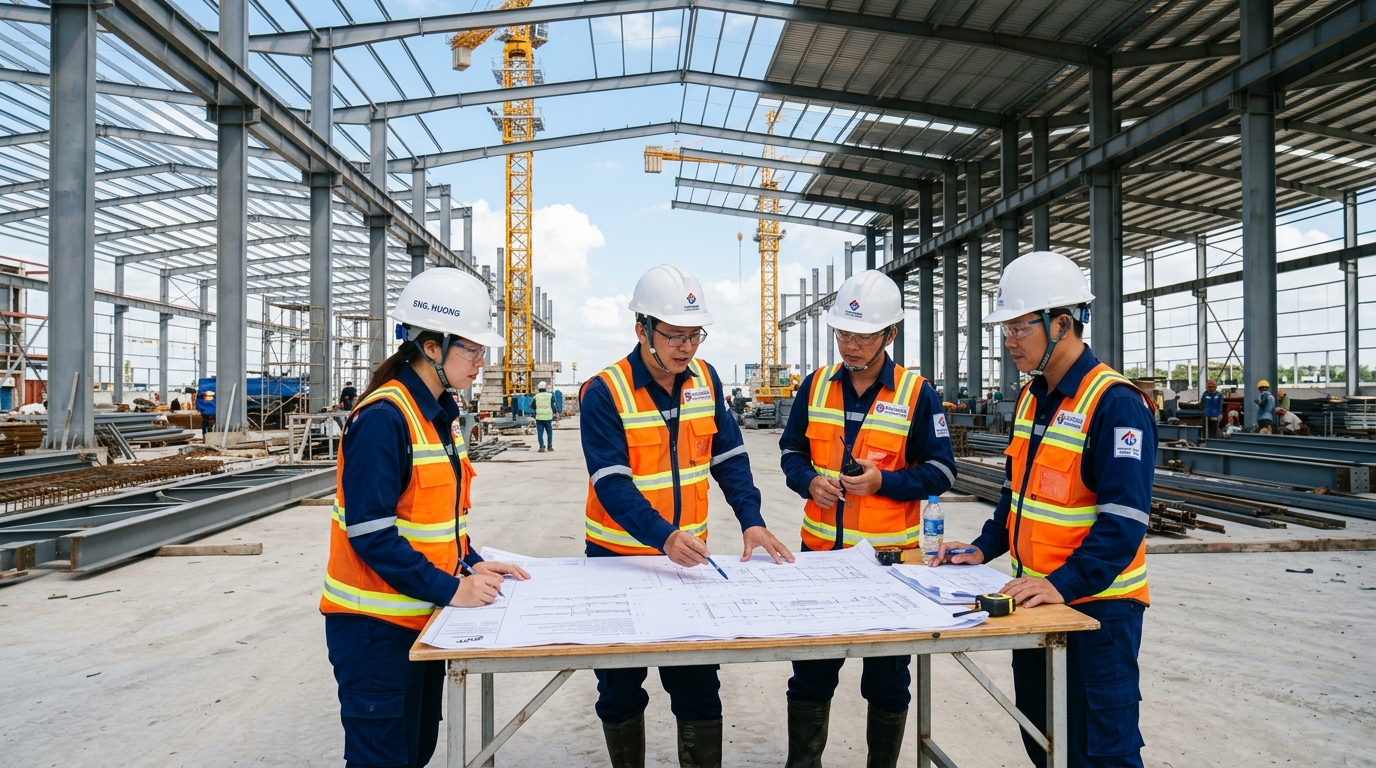
\includegraphics[height=62mm]{../../public/engineer-team-site.jpg}};
    \fill[TTCDeepNavy,opacity=.28] (0,87) rectangle (58,149);
  \end{scope}
  \node[anchor=west,text=TTCCyan,font=\fontsize{7}{8}\selectfont\bfseries] at (7,78)
    {STOP WORK AUTHORITY};
  \node[anchor=west,text=white,font=\fontsize{22}{23}\selectfont\bfseries] at (7,63)
    {STOP};
  \node[anchor=west,text=TTCRed!85!white,font=\fontsize{22}{23}\selectfont\bfseries] at (7,48)
    {WORK};
  \node[anchor=north west,text width=44mm,align=left] at (7,37) {
    {\fontsize{6.8}{8.3}\selectfont\color{white!85!gray}
    Bất kỳ ai cũng có quyền dừng công việc khi điều kiện an toàn chưa đầy đủ.}\\[2mm]
    {\fontsize{7}{8.5}\selectfont\bfseries\color{TTCGold}
    PEOPLE BEFORE PRODUCTION}
  };

  % Right — hierarchy of controls
  \fill[white,rounded corners=3pt] (63,86) rectangle (186,149);
  \draw[TTCBorder,rounded corners=3pt,line width=.6pt] (63,86) rectangle (186,149);
  \node[anchor=west,text=TTCBlue,font=\fontsize{8}{9.5}\selectfont\bfseries] at (69,141)
    {\faShield*\quad THỨ TỰ ƯU TIÊN KIỂM SOÁT RỦI RO};

  \fill[TTCRed] (69,124) rectangle (180,136);
  \fill[TTCBlue] (74,111) rectangle (175,123);
  \fill[TTCCyan] (79,98) rectangle (170,110);
  \fill[TTCGold] (84,85) rectangle (165,97);
  \node[anchor=west,text=white,font=\fontsize{7}{8}\selectfont\bfseries] at (73,130) {01 • ELIMINATE — Loại bỏ nguy cơ ngay từ biện pháp};
  \node[anchor=west,text=white,font=\fontsize{7}{8}\selectfont\bfseries] at (78,117) {02 • ENGINEER — Rào chắn, sàn thao tác, chống rơi};
  \node[anchor=west,text=white,font=\fontsize{7}{8}\selectfont\bfseries] at (83,104) {03 • PERMIT — JSA, giấy phép và người giám sát};
  \node[anchor=west,text=white,font=\fontsize{7}{8}\selectfont\bfseries] at (88,91) {04 • PPE — Lớp bảo vệ cuối cùng};

  % Right — daily safety cycle
  \fill[TTCLightBlue,rounded corners=3pt] (63,29) rectangle (186,81);
  \draw[TTCBorder,rounded corners=3pt,line width=.6pt] (63,29) rectangle (186,81);
  \node[anchor=west,text=TTCBlue,font=\fontsize{8}{9.5}\selectfont\bfseries] at (69,73)
    {\faClock\quad DAILY SAFETY CONTROL CYCLE};
  \draw[TTCBlue!35!white,line width=1pt] (76,50) -- (175,50);
  \foreach \x/\n/\t in {77/01/PLAN,102/02/TALK,127/03/VERIFY,152/04/WORK,175/05/CLOSE}{
    \fill[white] (\x,50) circle (4.5);
    \draw[TTCBlue,line width=.75pt] (\x,50) circle (4.5);
    \node[text=TTCRed,font=\fontsize{5.8}{6.5}\selectfont\bfseries] at (\x,50) {\n};
    \node[anchor=north,align=center,text width=22mm] at (\x,42)
      {{\fontsize{6}{7.2}\selectfont\bfseries\color{TTCBlue} \t}};
  }
  \node[anchor=west,text=TTCTextMuted,font=\fontsize{6}{7.3}\selectfont] at (70,33)
    {JSA / Method → Toolbox Talk → PPE \& thiết bị → Giám sát → Đóng hành động};

  % Emergency row
  \fill[white,rounded corners=3pt] (63,0) rectangle (186,24);
  \draw[TTCBorder,rounded corners=3pt,line width=.6pt] (63,0) rectangle (186,24);
  \node[anchor=west,text=TTCRed,font=\fontsize{8}{9.5}\selectfont\bfseries] at (69,16)
    {\faFireExtinguisher\quad EMERGENCY READY};
  \node[anchor=west,text=TTCTextDark,font=\fontsize{6.4}{7.8}\selectfont] at (69,7)
    {Báo động • Cô lập • Sơ tán • Sơ cứu • Điều tra • Phòng ngừa tái diễn};
\end{tikzpicture}

\vspace{3mm}

% LIFE-SAVING RULES
\noindent
\begin{tikzpicture}[x=1mm,y=1mm]
  \path[use as bounding box] (0,0) rectangle (186,48);
  \fill[white,rounded corners=3pt] (0,0) rectangle (186,48);
  \draw[TTCBorder,rounded corners=3pt,line width=.6pt] (0,0) rectangle (186,48);
  \node[anchor=west,text=TTCBlue,font=\fontsize{8}{9.5}\selectfont\bfseries] at (7,40)
    {\faHandPaper\quad 5 LIFE-SAVING RULES};
  \foreach \x in {37.2,74.4,111.6,148.8}{\draw[TTCBorder] (\x,6) -- (\x,31);}
  \node[align=center,text width=32mm] at (18.6,18) {
    {\fontsize{7.3}{8.5}\selectfont\bfseries\color{TTCRed} TRÊN CAO}\\[-.2mm]
    {\fontsize{5.8}{7}\selectfont 2 móc • lifeline • lưới hứng}
  };
  \node[align=center,text width=32mm] at (55.8,18) {
    {\fontsize{7.3}{8.5}\selectfont\bfseries\color{TTCBlue} NÂNG HẠ}\\[-.2mm]
    {\fontsize{5.8}{7}\selectfont Vùng cấm • tín hiệu • rigging}
  };
  \node[align=center,text width=32mm] at (93,18) {
    {\fontsize{7.3}{8.5}\selectfont\bfseries\color{TTCCyan} ĐIỆN}\\[-.2mm]
    {\fontsize{5.8}{7}\selectfont ELCB • tiếp địa • lock-out}
  };
  \node[align=center,text width=32mm] at (130.2,18) {
    {\fontsize{7.3}{8.5}\selectfont\bfseries\color{TTCGold} HÀN CẮT}\\[-.2mm]
    {\fontsize{5.8}{7}\selectfont Fire watch • chắn xỉ • permit}
  };
  \node[align=center,text width=32mm] at (167.4,18) {
    {\fontsize{7.3}{8.5}\selectfont\bfseries\color{TTCBlue} HỐ ĐÀO}\\[-.2mm]
    {\fontsize{5.8}{7}\selectfont Rào chắn • chống sạt • lối thoát}
  };
\end{tikzpicture}
\end{minipage}
\newpage

% ============================================================
% TRANG 20: SỔ DANH MỤC DỰ ÁN TIÊU BIỂU 01--08
% ============================================================
\AddToShipoutPictureFG*{%
  \AtPageUpperLeft{%
    \begin{tikzpicture}[x=1mm,y=1mm]
      \path[use as bounding box] (0,0) rectangle (0,0);
      \fill[TTCDeepNavy] (0,0) rectangle (210,-10);
      \fill[TTCRed] (0,-10) rectangle (210,-11);
      \node[anchor=west,text=white,font=\fontsize{7.5}{9}\selectfont\bfseries] at (12,-5)
        {\faBuilding\quad CÔNG TY CỔ PHẦN CÔNG NGHỆ XÂY DỰNG TÂN THÀNH CÔNG \textbullet\ TTC JSC};
      \node[anchor=east,text=TTCCyan,font=\fontsize{7.5}{9}\selectfont\bfseries] at (198,-5)
        {DANH MỤC DỰ ÁN TIÊU BIỂU • 01--08};
    \end{tikzpicture}%
  }%
  \AtPageLowerLeft{%
    \begin{tikzpicture}[x=1mm,y=1mm]
      \path[use as bounding box] (0,0) rectangle (0,0);
      \fill[TTCDeepNavy] (0,0) rectangle (210,8);
      \fill[TTCCyan] (0,8) rectangle (210,8.8);
      \node[anchor=west,text=white,font=\fontsize{6.8}{8}\selectfont] at (12,4)
        {\faPhone*\ +84 976 447 766 \quad\textbullet\quad \faEnvelope\ info@tanthanhcongjsc.com \quad\textbullet\quad \faGlobe\ https://tanthanhcongjsc.com};
      \node[anchor=east,text=white,font=\fontsize{7}{8}\selectfont\bfseries] at (198,4)
        {Trang 20};
    \end{tikzpicture}%
  }%
}

\begin{minipage}[t][246mm]{\textwidth}
\secbrand{Danh Mục Dự Án Công Nghiệp Tiêu Biểu}{Tám công trình đại diện • Thông tin cô đọng • Dễ đối chiếu}

{\fontsize{15}{17}\selectfont\bfseries\color{TTCBlue}
QUY MÔ • ĐỊA ĐIỂM • PHẠM VI CÔNG VIỆC\par}
\vspace{1mm}
{\fontsize{7.5}{9}\selectfont\color{TTCTextMuted}
Danh sách được trình bày theo một cấu trúc thống nhất để người đọc nhận biết nhanh vai trò của TTC tại từng dự án.\par}
\vspace{3mm}

\noindent
\begin{tikzpicture}[x=1mm,y=1mm]
  \path[use as bounding box] (0,0) rectangle (186,188);
  \fill[white,rounded corners=3pt] (0,0) rectangle (186,188);
  \draw[TTCBorder,rounded corners=3pt,line width=.7pt] (0,0) rectangle (186,188);

  % Tiêu đề cột
  \fill[TTCDeepNavy,rounded corners=3pt] (0,176) rectangle (186,188);
  \node[text=white,font=\fontsize{6.5}{7.5}\selectfont\bfseries] at (5,182) {STT};
  \node[anchor=west,text=white,font=\fontsize{6.5}{7.5}\selectfont\bfseries] at (14,182) {DỰ ÁN / CHỦ ĐẦU TƯ};
  \node[text=white,font=\fontsize{6.5}{7.5}\selectfont\bfseries] at (84,182) {QUY MÔ};
  \node[anchor=west,text=white,font=\fontsize{6.5}{7.5}\selectfont\bfseries] at (96,182) {ĐỊA ĐIỂM};
  \node[anchor=west,text=white,font=\fontsize{6.5}{7.5}\selectfont\bfseries] at (129,182) {PHẠM VI TTC};

  \newcommand{\projectrowa}[8]{%
    \fill[#8] (0,{#1-11}) rectangle (186,{#1+11});
    \fill[TTCBlue] (0,{#1-11}) rectangle (10,{#1+11});
    \node[text=white,font=\fontsize{7}{8}\selectfont\bfseries] at (5,#1) {#2};
    \node[anchor=west,text width=53mm,align=left] at (14,#1) {
      {\fontsize{7.2}{8.4}\selectfont\bfseries\color{TTCBlue} #3}\\[-.2mm]
      {\fontsize{5.8}{7}\selectfont\color{TTCTextMuted} #4}
    };
    \node[align=center,text width=20mm] at (84,#1)
      {{\fontsize{7}{8.2}\selectfont\bfseries\color{TTCTextDark} #5}};
    \node[anchor=west,text width=29mm,align=left] at (96,#1)
      {{\fontsize{5.9}{7.1}\selectfont\color{TTCTextDark} #6}};
    \node[anchor=west,text width=50mm,align=left] at (129,#1)
      {{\fontsize{6}{7.2}\selectfont\color{TTCTextDark} #7}};
    \draw[TTCBorder,line width=.45pt] (10,{#1-11}) -- (186,{#1-11});
  }

  \projectrowa{165}{01}{Tổ hợp NM Gạch Hồng Trang}{Gạch Hồng Trang • Việt Nam}{100.000 m$^2$}{Lập Thạch\\Vĩnh Phúc}{Tổng thầu EPC • Fast-track 6,5 tháng}{TTCLightBlue}
  \projectrowa{143}{02}{Nhà máy May Sông Hồng 7}{May Sông Hồng • Việt Nam}{68.000 m$^2$}{Hải Hậu\\Nam Định}{Thiết kế và thi công • Sàn hai tầng tải nặng}{white}
  \projectrowa{121}{03}{Tổ hợp NM Japfa Comfeed}{Japfa • Indonesia}{50.000 m$^2$}{Vĩnh Phúc\\Thái Bình}{Kết cấu silo cao 45 m • Xưởng CNC}{TTCLightBlue}
  \projectrowa{99}{04}{NM Thức Ăn Chăn Nuôi CP}{C.P • Thái Lan}{35.000 m$^2$}{Đồng Văn\\Hà Nam}{Xưởng sản xuất • Kho bảo quản}{white}
  \projectrowa{77}{05}{Nhà máy Daeyun ST Vina}{Daeyun • Hàn Quốc}{20.000 m$^2$}{Bá Thiện 2\\Vĩnh Phúc}{Xưởng sạch • Sàn chống tĩnh điện}{TTCLightBlue}
  \projectrowa{55}{06}{Nhà máy Dây Cáp Sumidenso}{Sumitomo • Nhật Bản}{15.015 m$^2$}{Sông Hậu\\Hậu Giang}{Nhà máy dây cáp ô tô • Hệ PCCC}{white}
  \projectrowa{33}{07}{Xưởng Sản Xuất Foxconn}{Foxconn • Đài Loan}{12.000 m$^2$}{Quế Võ\\Bắc Ninh}{Kết cấu vượt nhịp • Lắp dựng nhà xưởng cao}{TTCLightBlue}
  \projectrowa{11}{08}{Tổ hợp Logistics BW Industrial}{BW Industrial • Singapore}{45.000 m$^2$}{Yên Phong\\Bắc Ninh}{Tổng thầu kho thông minh • Sàn siêu phẳng}{white}
\end{tikzpicture}

\vspace{3mm}

\noindent
\begin{tikzpicture}[x=1mm,y=1mm]
  \path[use as bounding box] (0,0) rectangle (186,35);
  \fill[TTCDeepNavy,rounded corners=3pt] (0,0) rectangle (186,35);
  \node[anchor=west,text=TTCCyan,font=\fontsize{6.2}{7.2}\selectfont\bfseries]
    at (7,29) {NĂNG LỰC ĐƯỢC CHỨNG MINH QUA DANH MỤC};
  \foreach \x in {46.5,93,139.5}{\draw[white!25!gray] (\x,5) -- (\x,23);}
  \node[align=center,text width=40mm] at (23.25,14) {
    {\fontsize{8.2}{9.5}\selectfont\bfseries\color{white} EPC / DESIGN--BUILD}\\[-.2mm]
    {\fontsize{5.9}{7.1}\selectfont\color{white!75!gray}Một đầu mối xuyên suốt}
  };
  \node[align=center,text width=40mm] at (69.75,14) {
    {\fontsize{8.2}{9.5}\selectfont\bfseries\color{white} KẾT CẤU \& PEB}\\[-.2mm]
    {\fontsize{5.9}{7.1}\selectfont\color{white!75!gray}Nhịp lớn • tải nặng • silo}
  };
  \node[align=center,text width=40mm] at (116.25,14) {
    {\fontsize{8.2}{9.5}\selectfont\bfseries\color{white} SÀN CÔNG NGHIỆP}\\[-.2mm]
    {\fontsize{5.9}{7.1}\selectfont\color{white!75!gray}Sàn tải nặng • sàn phẳng}
  };
  \node[align=center,text width=40mm] at (162.75,14) {
    {\fontsize{8.2}{9.5}\selectfont\bfseries\color{white} MEP / PCCC}\\[-.2mm]
    {\fontsize{5.9}{7.1}\selectfont\color{white!75!gray}Tích hợp theo vận hành}
  };
\end{tikzpicture}
\end{minipage}
\newpage

% ============================================================
% TRANG 21: SỔ DANH MỤC DỰ ÁN TIÊU BIỂU 09--16
% ============================================================
\noindent\mbox{}\par\vspace{-\baselineskip}
\pageheaderbar{DANH MỤC DỰ ÁN TIÊU BIỂU • 09--16}{Trang 21}
\pagefooterbar{Trang 21}

\begin{minipage}[t][246mm]{\textwidth}
\secbrand{Danh Mục Dự Án FDI Và Công Nghiệp Phụ Trợ}{Tám công trình tiếp theo • Nhà đầu tư đa quốc gia • Yêu cầu chuyên biệt}

{\fontsize{15}{17}\selectfont\bfseries\color{TTCBlue}
NHÀ ĐẦU TƯ • CHUYÊN NGÀNH • GIẢI PHÁP TRIỂN KHAI\par}
\vspace{1mm}
{\fontsize{7.5}{9}\selectfont\color{TTCTextMuted}
Danh mục thể hiện kinh nghiệm triển khai nhà máy thực phẩm, điện tử, cơ khí, logistics và năng lượng.\par}
\vspace{3mm}

\noindent
\begin{tikzpicture}[x=1mm,y=1mm]
  \path[use as bounding box] (0,0) rectangle (186,188);
  \fill[white,rounded corners=3pt] (0,0) rectangle (186,188);
  \draw[TTCBorder,rounded corners=3pt,line width=.7pt] (0,0) rectangle (186,188);

  \fill[TTCDeepNavy,rounded corners=3pt] (0,176) rectangle (186,188);
  \node[text=white,font=\fontsize{6.5}{7.5}\selectfont\bfseries] at (5,182) {STT};
  \node[anchor=west,text=white,font=\fontsize{6.5}{7.5}\selectfont\bfseries] at (14,182) {DỰ ÁN / CHỦ ĐẦU TƯ};
  \node[text=white,font=\fontsize{6.5}{7.5}\selectfont\bfseries] at (84,182) {QUY MÔ};
  \node[anchor=west,text=white,font=\fontsize{6.5}{7.5}\selectfont\bfseries] at (96,182) {ĐỊA ĐIỂM};
  \node[anchor=west,text=white,font=\fontsize{6.5}{7.5}\selectfont\bfseries] at (129,182) {PHẠM VI TTC};

  \newcommand{\projectrowb}[8]{%
    \fill[#8] (0,{#1-11}) rectangle (186,{#1+11});
    \fill[TTCBlue] (0,{#1-11}) rectangle (10,{#1+11});
    \node[text=white,font=\fontsize{7}{8}\selectfont\bfseries] at (5,#1) {#2};
    \node[anchor=west,text width=53mm,align=left] at (14,#1) {
      {\fontsize{7.2}{8.4}\selectfont\bfseries\color{TTCBlue} #3}\\[-.2mm]
      {\fontsize{5.8}{7}\selectfont\color{TTCTextMuted} #4}
    };
    \node[align=center,text width=20mm] at (84,#1)
      {{\fontsize{7}{8.2}\selectfont\bfseries\color{TTCTextDark} #5}};
    \node[anchor=west,text width=29mm,align=left] at (96,#1)
      {{\fontsize{5.9}{7.1}\selectfont\color{TTCTextDark} #6}};
    \node[anchor=west,text width=50mm,align=left] at (129,#1)
      {{\fontsize{6}{7.2}\selectfont\color{TTCTextDark} #7}};
    \draw[TTCBorder,line width=.45pt] (10,{#1-11}) -- (186,{#1-11});
  }

  \projectrowb{165}{09}{NM Chăn Nuôi New Hope}{New Hope • Singapore}{32.000 m$^2$}{Quang Châu\\Bắc Giang}{Silo ngũ cốc • Trạm điện biến áp}{TTCLightBlue}
  \projectrowb{143}{10}{NM Cơ Khí Shinjo Vina}{Shinjo • Nhật Bản}{18.500 m$^2$}{VSIP\\Bắc Ninh}{Xưởng cơ khí chính xác • Dầm cầu trục 15T}{white}
  \projectrowb{121}{11}{NM Điện Tử Towada}{Towada • Nhật Bản}{16.000 m$^2$}{Phúc Điền\\Hải Dương}{Lắp ráp vi mạch • Phòng sạch ISO}{TTCLightBlue}
  \projectrowb{99}{12}{NM Bao Bì Toyo Seikan}{Toyo Seikan • Nhật Bản}{22.000 m$^2$}{Tiên Sơn\\Bắc Ninh}{Tổng thầu EPC • Xưởng bao bì • Sàn phẳng}{white}
  \projectrowb{77}{13}{Xưởng May Fami Vina}{Fami Garment • Hàn Quốc}{28.000 m$^2$}{Thụy Vân\\Phú Thọ}{Nhà xưởng may hai tầng • Hệ HVAC}{TTCLightBlue}
  \projectrowb{55}{14}{Kho Logistics Yusen}{Yusen • Nhật Bản}{25.000 m$^2$}{Đình Vũ\\Hải Phòng}{Kho ngoại quan • Cụm sàn nâng hàng}{white}
  \projectrowb{33}{15}{NM Thực Phẩm A-One}{Saigon Ve Wong • Đài Loan}{30.000 m$^2$}{Sóng Thần 2\\Bình Dương}{Xưởng chế biến thực phẩm • Chuẩn HACCP}{TTCLightBlue}
  \projectrowb{11}{16}{NM Năng Lượng Sơn Hà}{Sơn Hà • Việt Nam}{24.000 m$^2$}{Thuận Thành\\Bắc Ninh}{Xưởng sản xuất bồn • Pin mặt trời}{white}
\end{tikzpicture}

\vspace{3mm}

\noindent
\begin{tikzpicture}[x=1mm,y=1mm]
  \path[use as bounding box] (0,0) rectangle (186,35);
  \fill[TTCDeepNavy,rounded corners=3pt] (0,0) rectangle (186,35);
  \node[anchor=west,text=TTCCyan,font=\fontsize{6.2}{7.2}\selectfont\bfseries]
    at (7,29) {TỪ DANH MỤC ĐẾN 6 HỒ SƠ DỰ ÁN • TRANG 22--27};
  \foreach \x in {62,124}{\draw[white!25!gray] (\x,5) -- (\x,23);}
  \node[align=center,text width=53mm] at (31,14) {
    {\fontsize{7.8}{9.2}\selectfont\bfseries\color{white} HỒNG TRANG • SÔNG HỒNG 7}\\[-.2mm]
    {\fontsize{6}{7.2}\selectfont\color{white!75!gray}EPC nhịp lớn • nhà xưởng hai tầng}
  };
  \node[align=center,text width=53mm] at (93,14) {
    {\fontsize{7.8}{9.2}\selectfont\bfseries\color{white} JAPFA • DAEYUN}\\[-.2mm]
    {\fontsize{6}{7.2}\selectfont\color{white!75!gray}Công trình process • phòng sạch}
  };
  \node[align=center,text width=53mm] at (155,14) {
    {\fontsize{7.8}{9.2}\selectfont\bfseries\color{white} SUMIDENSO • FOXCONN}\\[-.2mm]
    {\fontsize{6}{7.2}\selectfont\color{white!75!gray}Bàn giao chất lượng • nhà xưởng điện tử}
  };
\end{tikzpicture}
\end{minipage}
\newpage

% ============================================================
% TRANG 22: FLAGSHIP CASE -- NHÀ MÁY GẠCH HỒNG TRANG
% ============================================================
\noindent\mbox{}\par\vspace{-\baselineskip}
\casepagebars{DỰ ÁN TIÊU BIỂU • HỒNG TRANG}{Trang 22}

\begin{minipage}[t][246mm]{\textwidth}
\secbrand{Hồ Sơ Dự Án 01: Nhà Máy Gạch Hồng Trang}{Flagship EPC case • Large-span industrial facility • Lập Thạch, Vĩnh Phúc}

\noindent
\begin{tikzpicture}[x=1mm,y=1mm]
  \path[use as bounding box] (0,0) rectangle (186,220);

  % Ảnh dự án nhỏ gọn, đúng với độ phân giải nguồn
  \begin{scope}
    \clip[rounded corners=4pt] (0,150) rectangle (70,220);
    \node[inner sep=0pt] at (35,185)
      {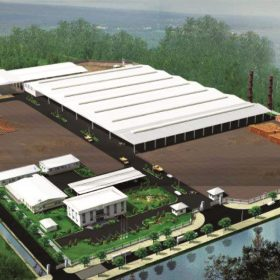
\includegraphics[width=70mm,height=70mm]{../../public/project-assets/hongtrang.jpg}};
    \fill[TTCDeepNavy,opacity=.88] (0,150) rectangle (70,161);
    \node[anchor=west,text=white,font=\fontsize{7}{8}\selectfont\bfseries]
      at (4,155.5) {ẢNH DỰ ÁN • LẬP THẠCH, VĨNH PHÚC};
  \end{scope}
  \draw[TTCBorder,rounded corners=4pt,line width=.7pt] (0,150) rectangle (70,220);

  % Tóm tắt điều hành
  \fill[TTCLightBlue,rounded corners=4pt] (74,150) rectangle (186,220);
  \draw[TTCBorder,rounded corners=4pt,line width=.7pt] (74,150) rectangle (186,220);
  \node[anchor=north west,text=TTCRed,font=\fontsize{7.5}{9}\selectfont\bfseries]
    at (80,214) {TỔNG THẦU EPC};
  \node[anchor=north west,text width=99mm,align=left,text=TTCBlue,
        font=\fontsize{14}{16}\selectfont\bfseries]
    at (80,207) {100.000 m$^2$ QUY HOẠCH};
  \draw[TTCBorder,line width=.55pt] (80,190) -- (180,190);
  \foreach \x in {113.3,146.6}{\draw[TTCBorder,line width=.5pt] (\x,163) -- (\x,186);}
  \node[align=center,text width=29mm] at (96.5,176) {
    {\fontsize{11}{12}\selectfont\bfseries\color{TTCRed}75.000 m$^2$}\\[-.5mm]
    {\fontsize{6.2}{7.4}\selectfont\color{TTCTextMuted}DIỆN TÍCH SÀN}};
  \node[align=center,text width=29mm] at (130,176) {
    {\fontsize{11}{12}\selectfont\bfseries\color{TTCBlue}NHỊP 42M}\\[-.5mm]
    {\fontsize{6.2}{7.4}\selectfont\color{TTCTextMuted}KHÔNG CỘT GIỮA}};
  \node[align=center,text width=29mm] at (163.5,176) {
    {\fontsize{11}{12}\selectfont\bfseries\color{TTCBlue}6,5 THÁNG}\\[-.5mm]
    {\fontsize{6.2}{7.4}\selectfont\color{TTCTextMuted}TIẾN ĐỘ THI CÔNG}};
  \node[anchor=south west,text width=99mm,align=left,text=TTCTextDark,
        font=\fontsize{7.4}{9}\selectfont]
    at (80,153) {\textbf{Phạm vi TTC:} Tổng thầu EPC; phối hợp thiết kế, kết cấu thép, hạ tầng và tổ chức thi công fast-track.};

  % Câu chuyện dự án: bài toán -- giải pháp -- kết quả
  \node[anchor=west,text=TTCBlue,font=\fontsize{8}{9.5}\selectfont\bfseries]
    at (0,143) {CÂU CHUYỆN DỰ ÁN • CHỈ GIỮ BA Ý CHÍNH};

  \fill[white,rounded corners=4pt] (0,79) rectangle (58,137);
  \draw[TTCBorder,rounded corners=4pt,line width=.7pt] (0,79) rectangle (58,137);
  \fill[TTCRed,rounded corners=2pt] (5,124) rectangle (16,133);
  \node[text=white,font=\fontsize{7}{8}\selectfont\bfseries] at (10.5,128.5) {01};
  \node[anchor=north west,text=TTCBlue,font=\fontsize{9}{10.5}\selectfont\bfseries]
    at (5,120) {BÀI TOÁN};
  \node[anchor=north west,text width=48mm,align=left,text=TTCTextDark,
        font=\fontsize{7.2}{9}\selectfont]
    at (5,110) {Dây chuyền lò nung cần mặt bằng liên tục, không bị chia cắt bởi cột giữa; đồng thời nhà xưởng phải thoát nhiệt hiệu quả.};

  \draw[-{Latex[length=2.5mm]},TTCCyan,line width=1pt] (59.5,108) -- (63,108);
  \fill[TTCDeepNavy,rounded corners=4pt] (64,79) rectangle (122,137);
  \node[text=TTCDeepNavy,fill=white,rounded corners=2pt,font=\fontsize{7}{8}\selectfont\bfseries,
        minimum width=11mm,minimum height=9mm] at (74.5,128.5) {02};
  \node[anchor=north west,text=white,font=\fontsize{9}{10.5}\selectfont\bfseries]
    at (69,120) {GIẢI PHÁP TTC};
  \node[anchor=north west,text width=48mm,align=left,text=white,
        font=\fontsize{7.2}{9}\selectfont]
    at (69,110) {Khung thép tiết diện thay đổi vượt nhịp 42 m; thông gió đối lưu đỉnh mái; các gói EPC được triển khai song song.};

  \draw[-{Latex[length=2.5mm]},TTCCyan,line width=1pt] (123.5,108) -- (127,108);
  \fill[TTCLightBlue,rounded corners=4pt] (128,79) rectangle (186,137);
  \draw[TTCBorder,rounded corners=4pt,line width=.7pt] (128,79) rectangle (186,137);
  \fill[TTCBlue,rounded corners=2pt] (133,124) rectangle (144,133);
  \node[text=white,font=\fontsize{7}{8}\selectfont\bfseries] at (138.5,128.5) {03};
  \node[anchor=north west,text=TTCBlue,font=\fontsize{9}{10.5}\selectfont\bfseries]
    at (133,120) {KẾT QUẢ};
  \node[anchor=north west,text width=48mm,align=left,text=TTCTextDark,
        font=\fontsize{7.2}{9}\selectfont]
    at (133,110) {Hoàn thành 75.000 m$^2$ sàn trong 6,5 tháng; bàn giao sớm 20 ngày theo hồ sơ năng lực hiện tại.};

  % Băng ghi nhớ
  \fill[white,rounded corners=4pt] (0,20) rectangle (186,70);
  \draw[TTCBorder,rounded corners=4pt,line width=.7pt] (0,20) rectangle (186,70);
  \node[anchor=west,text=TTCBlue,font=\fontsize{8}{9.5}\selectfont\bfseries]
    at (7,61) {BA ĐIỂM NGƯỜI ĐỌC CẦN NHỚ};
  \draw[TTCBorder] (62,27) -- (62,58);
  \draw[TTCBorder] (124,27) -- (124,58);
  \node[align=center,text width=52mm] at (31,42) {
    {\fontsize{12}{13}\selectfont\bfseries\color{TTCRed}42 MÉT}\\[-.5mm]
    {\fontsize{6.6}{8}\selectfont\color{TTCTextMuted}MẶT BẰNG SẢN XUẤT KHÔNG CỘT GIỮA}};
  \node[align=center,text width=52mm] at (93,42) {
    {\fontsize{12}{13}\selectfont\bfseries\color{TTCBlue}EPC SONG SONG}\\[-.5mm]
    {\fontsize{6.6}{8}\selectfont\color{TTCTextMuted}THIẾT KẾ • SẢN XUẤT • THI CÔNG}};
  \node[align=center,text width=52mm] at (155,42) {
    {\fontsize{12}{13}\selectfont\bfseries\color{TTCBlue}SỚM 20 NGÀY}\\[-.5mm]
    {\fontsize{6.6}{8}\selectfont\color{TTCTextMuted}SO VỚI MỐC CAM KẾT}};

  \fill[TTCDeepNavy,rounded corners=3pt] (0,0) rectangle (186,14);
  \node[anchor=west,text=white,font=\fontsize{7.4}{9}\selectfont\bfseries]
    at (7,7) {GIÁ TRỊ CỐT LÕI: KHÔNG GIAN SẢN XUẤT LIÊN TỤC • TIẾN ĐỘ CÓ KIỂM SOÁT};
\end{tikzpicture}
\end{minipage}
\newpage

% ============================================================
% TRANG 23: ENGINEERING CASE -- NHÀ MÁY MAY SÔNG HỒNG 7
% ============================================================
\noindent\mbox{}\par\vspace{-\baselineskip}
\casepagebars{GIẢI PHÁP KỸ THUẬT • SÔNG HỒNG 7}{Trang 23}

\begin{minipage}[t][246mm]{\textwidth}
\secbrand{Hồ Sơ Dự Án 02: Nhà Máy May Sông Hồng 7}{Engineering anatomy • Two-storey heavy-duty factory • Hải Hậu, Nam Định}

\noindent
\begin{tikzpicture}[x=1mm,y=1mm]
  \path[use as bounding box] (0,0) rectangle (186,220);

  % Phối cảnh và thẻ dữ liệu
  \begin{scope}
    \clip[rounded corners=4pt] (0,148) rectangle (104,220);
    \node[inner sep=0pt] at (52,184)
      {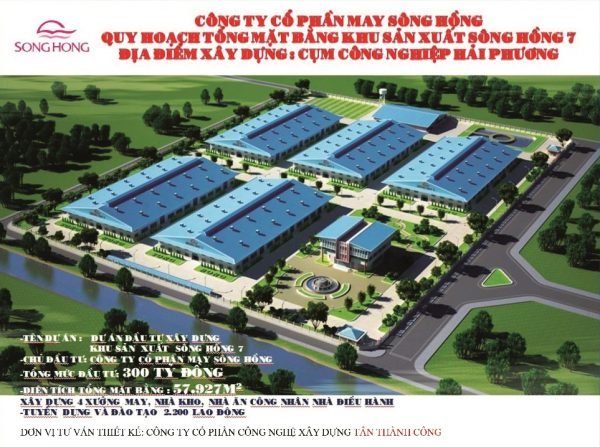
\includegraphics[width=104mm,height=77.5mm]{../../public/project-assets/songhong7.jpg}};
    \fill[TTCDeepNavy,opacity=.88] (0,148) rectangle (104,160);
    \node[anchor=west,text=white,font=\fontsize{7}{8}\selectfont\bfseries]
      at (4,154) {PHỐI CẢNH DỰ ÁN • HẢI HẬU, NAM ĐỊNH};
  \end{scope}
  \draw[TTCBorder,rounded corners=4pt,line width=.7pt] (0,148) rectangle (104,220);

  \fill[TTCDeepNavy,rounded corners=4pt] (108,148) rectangle (186,220);
  \node[anchor=north west,text=TTCCyan,font=\fontsize{7.2}{8.5}\selectfont\bfseries]
    at (114,214) {TÓM TẮT DỰ ÁN};
  \node[anchor=north west,text=white,font=\fontsize{15}{16}\selectfont\bfseries]
    at (114,205) {68.000 m$^2$};
  \node[anchor=north west,text=white!75!gray,font=\fontsize{6.5}{8}\selectfont]
    at (114,190) {TỔNG DIỆN TÍCH SÀN};
  \draw[white!25!gray] (114,183) -- (180,183);
  \node[anchor=north west,text width=62mm,align=left,text=white,
        font=\fontsize{7.2}{9}\selectfont]
    at (114,178) {\textbf{Kết cấu:} Nhà xưởng hai tầng\\[1mm]
                  \textbf{Tải trọng thiết kế:} 1.200 kg/m$^2$\\[1mm]
                  \textbf{Tiến độ:} 180 ngày\\[1mm]
                  \textbf{Vai trò TTC:} Thiết kế và thi công};

  % Sơ đồ kỹ thuật khác biệt với trang trước
  \node[anchor=west,text=TTCBlue,font=\fontsize{8}{9.5}\selectfont\bfseries]
    at (0,140) {SƠ ĐỒ NGUYÊN LÝ • ĐƯỜNG TRUYỀN TẢI VÀ KIỂM SOÁT RUNG};
  \fill[TTCLightBlue,rounded corners=4pt] (0,53) rectangle (186,134);
  \draw[TTCBorder,rounded corners=4pt,line width=.7pt] (0,53) rectangle (186,134);

  % Khung hai tầng
  \draw[TTCBlue,line width=1.2pt] (10,67) -- (132,67);
  \draw[TTCBlue,line width=2pt] (12,94) -- (130,94);
  \draw[TTCBlue,line width=1.2pt] (12,122) -- (71,130) -- (130,122);
  \foreach \x in {16,44,72,100,128}{
    \draw[TTCBlue,line width=1.2pt] (\x,67) -- (\x,122);
  }
  \foreach \x in {26,54,82,110}{
    \fill[white] (\x,98) rectangle +(15,7);
    \draw[TTCBorder] (\x,98) rectangle +(15,7);
    \draw[-{Latex[length=2mm]},TTCRed,line width=.8pt] (\x+7.5,108) -- (\x+7.5,96);
  }
  \node[anchor=west,text=TTCRed,font=\fontsize{6.5}{8}\selectfont\bfseries]
    at (16,112) {TẢI TRỌNG ĐỘNG TỪ CỤM MÁY SẢN XUẤT};
  \draw[TTCCyan,line width=1.2pt,dashed] (17,87) -- (127,87);
  \node[anchor=west,text=TTCCyan,font=\fontsize{6.3}{7.5}\selectfont\bfseries]
    at (19,82) {TUYẾN MEP / HVAC PHỐI HỢP DƯỚI SÀN};
  \draw[<->,>=Latex,TTCBlue,line width=.8pt] (16,60) -- (128,60);
  \node[fill=TTCLightBlue,text=TTCBlue,font=\fontsize{6.5}{8}\selectfont\bfseries]
    at (72,60) {KHÔNG GIAN SẢN XUẤT HAI TẦNG};

  % Chú giải bên phải
  \draw[TTCBorder] (138,60) -- (138,127);
  \node[anchor=north west,text=TTCBlue,font=\fontsize{7.2}{8.5}\selectfont\bfseries]
    at (145,124) {3 QUYẾT ĐỊNH THIẾT KẾ};
  \node[anchor=north west,text width=34mm,align=left,text=TTCTextDark,
        font=\fontsize{6.7}{8.3}\selectfont]
    at (145,114) {\textbf{01 • Sàn liên hợp}\newline
                  Deck mạ kẽm và bê tông cốt thép tạo mặt sàn tải nặng.};
  \node[anchor=north west,text width=34mm,align=left,text=TTCTextDark,
        font=\fontsize{6.7}{8.3}\selectfont]
    at (145,92) {\textbf{02 • Kiểm soát rung}\newline
                  Phân vùng tải và đường truyền lực rõ ràng theo khu máy.};
  \node[anchor=north west,text width=34mm,align=left,text=TTCTextDark,
        font=\fontsize{6.7}{8.3}\selectfont]
    at (145,70) {\textbf{03 • Phối hợp MEP}\newline
                  Dành trước không gian HVAC và tuyến kỹ thuật dưới sàn.};

  % Ba ý ghi nhớ
  \fill[white,rounded corners=3pt] (0,9) rectangle (58,45);
  \draw[TTCBorder,rounded corners=3pt] (0,9) rectangle (58,45);
  \node[anchor=north west,text=TTCRed,font=\fontsize{8}{9}\selectfont\bfseries]
    at (5,39) {01 • TẢI NẶNG};
  \node[anchor=north west,text width=48mm,text=TTCTextDark,font=\fontsize{6.8}{8.4}\selectfont]
    at (5,30) {Sàn tầng hai được tổ chức theo khu vực tải và thiết bị.};

  \fill[white,rounded corners=3pt] (64,9) rectangle (122,45);
  \draw[TTCBorder,rounded corners=3pt] (64,9) rectangle (122,45);
  \node[anchor=north west,text=TTCBlue,font=\fontsize{8}{9}\selectfont\bfseries]
    at (69,39) {02 • PHỐI HỢP};
  \node[anchor=north west,text width=48mm,text=TTCTextDark,font=\fontsize{6.8}{8.4}\selectfont]
    at (69,30) {Kết cấu và MEP được khóa giao diện trước khi triển khai.};

  \fill[white,rounded corners=3pt] (128,9) rectangle (186,45);
  \draw[TTCBorder,rounded corners=3pt] (128,9) rectangle (186,45);
  \node[anchor=north west,text=TTCBlue,font=\fontsize{8}{9}\selectfont\bfseries]
    at (133,39) {03 • TIẾN ĐỘ};
  \node[anchor=north west,text width=48mm,text=TTCTextDark,font=\fontsize{6.8}{8.4}\selectfont]
    at (133,30) {Chu kỳ kết cấu, sàn và cơ điện được triển khai theo nhịp lặp.};

  \fill[TTCDeepNavy,rounded corners=2pt] (0,0) rectangle (186,6);
\end{tikzpicture}
\end{minipage}
\newpage

% ============================================================
% TRANG 24: PROCESS CASE -- TỔ HỢP JAPFA COMFEED
% ============================================================
\noindent\mbox{}\par\vspace{-\baselineskip}
\casepagebars{CÔNG TRÌNH CÔNG NGHỆ • JAPFA COMFEED}{Trang 24}

\begin{minipage}[t][246mm]{\textwidth}
\secbrand{Hồ Sơ Dự Án 03: Tổ Hợp Japfa Comfeed}{Process-industry case • High-rise silo • Dynamic-load and dust control}

\noindent
\begin{tikzpicture}[x=1mm,y=1mm]
  \path[use as bounding box] (0,0) rectangle (186,220);

  % Ảnh nhỏ và bảng số liệu 2x2
  \begin{scope}
    \clip[rounded corners=4pt] (0,151) rectangle (68,219);
    \node[inner sep=0pt] at (34,185)
      {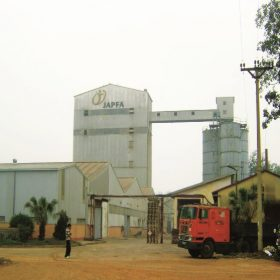
\includegraphics[width=68mm,height=68mm]{../../public/project-assets/japfa.jpg}};
    \fill[TTCDeepNavy,opacity=.9] (0,151) rectangle (68,162);
    \node[anchor=west,text=white,font=\fontsize{7}{8}\selectfont\bfseries]
      at (4,156.5) {ẢNH DỰ ÁN • JAPFA COMFEED};
  \end{scope}
  \draw[TTCBorder,rounded corners=4pt,line width=.7pt] (0,151) rectangle (68,219);

  \fill[TTCLightBlue,rounded corners=4pt] (72,151) rectangle (186,219);
  \draw[TTCBorder,rounded corners=4pt,line width=.7pt] (72,151) rectangle (186,219);
  \node[anchor=west,text=TTCBlue,font=\fontsize{8}{9.5}\selectfont\bfseries]
    at (78,211) {CỤM DỰ ÁN VĨNH PHÚC / THÁI BÌNH};
  \draw[TTCBorder] (129,158) -- (129,204);
  \draw[TTCBorder] (78,181) -- (180,181);
  \node[align=center,text width=45mm] at (103.5,193) {
    {\fontsize{12}{13}\selectfont\bfseries\color{TTCRed}50.000 m$^2$}\\[-.5mm]
    {\fontsize{6.2}{7.4}\selectfont\color{TTCTextMuted}DIỆN TÍCH QUY HOẠCH}};
  \node[align=center,text width=45mm] at (154.5,193) {
    {\fontsize{12}{13}\selectfont\bfseries\color{TTCBlue}SILO 45M}\\[-.5mm]
    {\fontsize{6.2}{7.4}\selectfont\color{TTCTextMuted}CHIỀU CAO CỤM THÁP}};
  \node[align=center,text width=45mm] at (103.5,169) {
    {\fontsize{12}{13}\selectfont\bfseries\color{TTCBlue}2.800 TẤN}\\[-.5mm]
    {\fontsize{6.2}{7.4}\selectfont\color{TTCTextMuted}KẾT CẤU THÉP PEB}};
  \node[align=center,text width=45mm] at (154.5,169) {
    {\fontsize{12}{13}\selectfont\bfseries\color{TTCBlue}165 NGÀY}\\[-.5mm]
    {\fontsize{6.2}{7.4}\selectfont\color{TTCTextMuted}TIẾN ĐỘ THI CÔNG}};

  % Câu chuyện theo chiều cao
  \node[anchor=west,text=TTCBlue,font=\fontsize{8}{9.5}\selectfont\bfseries]
    at (0,143) {CÂU CHUYỆN KỸ THUẬT • TỪ MÓNG ĐỘNG LỰC ĐẾN ĐỈNH SILO};
  \fill[TTCLightBlue,rounded corners=4pt] (0,56) rectangle (54,137);
  \draw[TTCBorder,rounded corners=4pt,line width=.7pt] (0,56) rectangle (54,137);

  % Tháp silo mô phỏng
  \fill[TTCBlue!10!white] (19,69) rectangle (42,123);
  \draw[TTCBlue,line width=1.1pt] (19,69) rectangle (42,123);
  \foreach \y in {80,91,102,113}{\draw[TTCBorder] (19,\y) -- (42,\y);}
  \draw[TTCBlue,line width=1.1pt] (16,69) -- (45,69);
  \fill[TTCDeepNavy] (12,62) rectangle (49,69);
  \draw[<->,>=Latex,TTCRed,line width=.9pt] (9,69) -- (9,123);
  \node[rotate=90,text=TTCRed,font=\fontsize{9}{10}\selectfont\bfseries]
    at (4,96) {45 MÉT};
  \node[text=TTCBlue,font=\fontsize{6.5}{7.5}\selectfont\bfseries]
    at (30.5,129) {CỤM SILO};
  \node[text=white,font=\fontsize{6.2}{7.2}\selectfont\bfseries]
    at (30.5,65.5) {MÓNG D800};

  % Ba rủi ro -- ba phản hồi
  \fill[white,rounded corners=3pt] (60,108) rectangle (186,137);
  \draw[TTCBorder,rounded corners=3pt] (60,108) rectangle (186,137);
  \fill[TTCRed] (60,108) rectangle (63,137);
  \node[anchor=north west,text=TTCBlue,font=\fontsize{8}{9}\selectfont\bfseries]
    at (69,132) {01 • TẢI ĐỘNG MÁY NGHIỀN};
  \node[anchor=north west,text width=108mm,text=TTCTextDark,font=\fontsize{6.9}{8.4}\selectfont]
    at (69,122) {Móng cọc khoan nhồi sâu D800 kết hợp lớp giảm chấn để kiểm soát rung truyền sang khu vực lân cận.};

  \fill[white,rounded corners=3pt] (60,76) rectangle (186,105);
  \draw[TTCBorder,rounded corners=3pt] (60,76) rectangle (186,105);
  \fill[TTCBlue] (60,76) rectangle (63,105);
  \node[anchor=north west,text=TTCBlue,font=\fontsize{8}{9}\selectfont\bfseries]
    at (69,100) {02 • LẮP DỰNG THEO CAO ĐỘ};
  \node[anchor=north west,text width=108mm,text=TTCTextDark,font=\fontsize{6.9}{8.4}\selectfont]
    at (69,90) {Chia tháp thành các phân đoạn lắp dựng; kiểm soát cao độ, độ thẳng đứng và liên kết tại từng điểm dừng kỹ thuật.};

  \fill[white,rounded corners=3pt] (60,44) rectangle (186,73);
  \draw[TTCBorder,rounded corners=3pt] (60,44) rectangle (186,73);
  \fill[TTCBlue] (60,44) rectangle (63,73);
  \node[anchor=north west,text=TTCBlue,font=\fontsize{8}{9}\selectfont\bfseries]
    at (69,68) {03 • BỤI VÀ AN TOÀN QUY TRÌNH};
  \node[anchor=north west,text width=108mm,text=TTCTextDark,font=\fontsize{6.9}{8.4}\selectfont]
    at (69,58) {Tích hợp thu gom bụi, thông gió và giải pháp xả áp theo yêu cầu vận hành ATEX / HACCP của dây chuyền.};

  % Chuỗi phạm vi TTC
  \fill[TTCDeepNavy,rounded corners=4pt] (0,0) rectangle (186,35);
  \node[anchor=west,text=TTCCyan,font=\fontsize{6.5}{8}\selectfont\bfseries]
    at (7,28) {PHẠM VI TRIỂN KHAI};
  \foreach \x in {46.5,93,139.5}{\draw[white!25!gray] (\x,6) -- (\x,25);}
  \node[align=center,text width=39mm,text=white,font=\fontsize{7.2}{8.5}\selectfont\bfseries]
    at (23.25,15) {MÓNG SÂU\\[-.5mm]{\fontsize{5.8}{7}\selectfont\color{white!70!gray}TẢI TĨNH + TẢI ĐỘNG}};
  \node[align=center,text width=39mm,text=white,font=\fontsize{7.2}{8.5}\selectfont\bfseries]
    at (69.75,15) {KẾT CẤU PEB\\[-.5mm]{\fontsize{5.8}{7}\selectfont\color{white!70!gray}SẢN XUẤT \& LẮP DỰNG}};
  \node[align=center,text width=39mm,text=white,font=\fontsize{7.2}{8.5}\selectfont\bfseries]
    at (116.25,15) {CỤM SILO\\[-.5mm]{\fontsize{5.8}{7}\selectfont\color{white!70!gray}KIỂM SOÁT CAO ĐỘ}};
  \node[align=center,text width=39mm,text=white,font=\fontsize{7.2}{8.5}\selectfont\bfseries]
    at (162.75,15) {HỆ THỐNG PHỤ TRỢ\\[-.5mm]{\fontsize{5.8}{7}\selectfont\color{white!70!gray}BỤI • ĐIỆN • AN TOÀN}};
\end{tikzpicture}
\end{minipage}
\newpage

% ============================================================
% TRANG 25: CLEANROOM CASE -- DAEYUN ST VINA
% ============================================================
\noindent\mbox{}\par\vspace{-\baselineskip}
\casepagebars{HỆ THỐNG PHÒNG SẠCH • DAEYUN ST VINA}{Trang 25}

\begin{minipage}[t][246mm]{\textwidth}
\secbrand{Hồ Sơ Dự Án 04: Nhà Máy Daeyun ST Vina}{Integrated cleanroom systems • KCN Bá Thiện 2, Vĩnh Phúc}

\noindent
\begin{tikzpicture}[x=1mm,y=1mm]
  \path[use as bounding box] (0,0) rectangle (186,220);

  % Phối cảnh ngang + thẻ dữ liệu dọc
  \begin{scope}
    \clip[rounded corners=4pt] (0,157) rectangle (118,219);
    \node[inner sep=0pt] at (59,188)
      {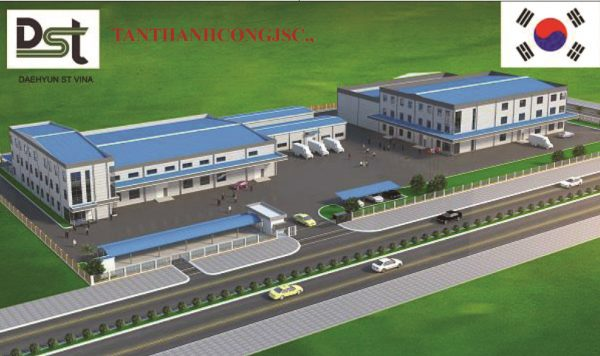
\includegraphics[width=118mm]{../../public/project-assets/daeyun.jpg}};
    \fill[TTCDeepNavy,opacity=.88] (0,157) rectangle (118,168);
    \node[anchor=west,text=white,font=\fontsize{7}{8}\selectfont\bfseries]
      at (4,162.5) {PHỐI CẢNH DỰ ÁN • KCN BÁ THIỆN 2};
  \end{scope}
  \draw[TTCBorder,rounded corners=4pt,line width=.7pt] (0,157) rectangle (118,219);

  \fill[TTCDeepNavy,rounded corners=4pt] (122,157) rectangle (186,219);
  \node[anchor=north west,text=TTCCyan,font=\fontsize{7}{8}\selectfont\bfseries]
    at (128,213) {THÔNG TIN DỰ ÁN};
  \node[anchor=north west,text=white,font=\fontsize{13}{14}\selectfont\bfseries]
    at (128,203) {20.000 m$^2$};
  \node[anchor=north west,text=white!70!gray,font=\fontsize{6}{7.2}\selectfont]
    at (128,190) {DIỆN TÍCH SÀN};
  \draw[white!25!gray] (128,184) -- (180,184);
  \node[anchor=north west,text width=48mm,align=left,text=white,
        font=\fontsize{6.8}{8.4}\selectfont]
    at (128,180) {\textbf{Phân loại:} Xưởng sạch\\
                  \textbf{Yêu cầu:} Class 10.000\\
                  \textbf{Tiến độ:} 140 ngày};

  % Bản đồ hệ thống
  \node[anchor=west,text=TTCBlue,font=\fontsize{8}{9.5}\selectfont\bfseries]
    at (0,149) {BẢN ĐỒ HỆ THỐNG • BỐN LỚP PHẢI HOẠT ĐỘNG NHƯ MỘT};
  \fill[TTCLightBlue,rounded corners=4pt] (0,57) rectangle (186,143);
  \draw[TTCBorder,rounded corners=4pt,line width=.7pt] (0,57) rectangle (186,143);

  % Trung tâm sản xuất
  \fill[TTCDeepNavy,rounded corners=4pt] (68,88) rectangle (118,116);
  \node[align=center,text=white,text width=42mm,font=\fontsize{8}{9.5}\selectfont\bfseries]
    at (93,102) {VÙNG SẢN XUẤT SẠCH\\[-.5mm]
    {\fontsize{6}{7.2}\selectfont\color{white!70!gray}ỔN ĐỊNH • KÍN • CHỐNG TĨNH ĐIỆN}};

  % Bốn mô-đun xung quanh
  \fill[white,rounded corners=3pt] (7,108) rectangle (58,136);
  \draw[TTCBorder,rounded corners=3pt] (7,108) rectangle (58,136);
  \node[anchor=north west,text=TTCBlue,font=\fontsize{7.5}{8.5}\selectfont\bfseries]
    at (12,131) {01 • BAO CHE KÍN};
  \node[anchor=north west,text width=41mm,text=TTCTextDark,font=\fontsize{6.4}{7.8}\selectfont]
    at (12,121) {Panel vách và trần hạn chế xâm nhập bụi, duy trì phân vùng áp suất.};

  \fill[white,rounded corners=3pt] (128,108) rectangle (179,136);
  \draw[TTCBorder,rounded corners=3pt] (128,108) rectangle (179,136);
  \node[anchor=north west,text=TTCBlue,font=\fontsize{7.5}{8.5}\selectfont\bfseries]
    at (133,131) {02 • AHU / HEPA};
  \node[anchor=north west,text width=41mm,text=TTCTextDark,font=\fontsize{6.4}{7.8}\selectfont]
    at (133,121) {Cấp và hồi khí có lọc; cân bằng lưu lượng theo từng khu vực chức năng.};

  \fill[white,rounded corners=3pt] (7,64) rectangle (58,92);
  \draw[TTCBorder,rounded corners=3pt] (7,64) rectangle (58,92);
  \node[anchor=north west,text=TTCRed,font=\fontsize{7.5}{8.5}\selectfont\bfseries]
    at (12,87) {03 • NHIỆT / ẨM};
  \node[anchor=north west,text width=41mm,text=TTCTextDark,font=\fontsize{6.4}{7.8}\selectfont]
    at (12,77) {Kiểm soát mục tiêu $\pm1^\circ$C và $\pm5\%$ theo yêu cầu dây chuyền.};

  \fill[white,rounded corners=3pt] (128,64) rectangle (179,92);
  \draw[TTCBorder,rounded corners=3pt] (128,64) rectangle (179,92);
  \node[anchor=north west,text=TTCBlue,font=\fontsize{7.5}{8.5}\selectfont\bfseries]
    at (133,87) {04 • SÀN ESD};
  \node[anchor=north west,text width=41mm,text=TTCTextDark,font=\fontsize{6.4}{7.8}\selectfont]
    at (133,77) {Vinyl dẫn điện và mạng tiếp địa hỗ trợ kiểm soát phóng tĩnh điện.};

  \draw[-{Latex[length=2mm]},TTCCyan,line width=.9pt] (58,122) -- (68,108);
  \draw[-{Latex[length=2mm]},TTCCyan,line width=.9pt] (128,122) -- (118,108);
  \draw[-{Latex[length=2mm]},TTCCyan,line width=.9pt] (58,78) -- (68,94);
  \draw[-{Latex[length=2mm]},TTCCyan,line width=.9pt] (128,78) -- (118,94);

  % Kết quả ghi nhớ
  \fill[white,rounded corners=3pt] (0,10) rectangle (58,48);
  \draw[TTCBorder,rounded corners=3pt] (0,10) rectangle (58,48);
  \node[align=center,text width=48mm] at (29,29) {
    {\fontsize{10}{11}\selectfont\bfseries\color{TTCRed}CLASS 10.000}\\[-.5mm]
    {\fontsize{6.4}{7.6}\selectfont\color{TTCTextMuted}YÊU CẦU MÔI TRƯỜNG SẠCH}};

  \fill[white,rounded corners=3pt] (64,10) rectangle (122,48);
  \draw[TTCBorder,rounded corners=3pt] (64,10) rectangle (122,48);
  \node[align=center,text width=48mm] at (93,29) {
    {\fontsize{10}{11}\selectfont\bfseries\color{TTCBlue}ESD VINYL}\\[-.5mm]
    {\fontsize{6.4}{7.6}\selectfont\color{TTCTextMuted}BẢO VỆ LINH KIỆN ĐIỆN TỬ}};

  \fill[white,rounded corners=3pt] (128,10) rectangle (186,48);
  \draw[TTCBorder,rounded corners=3pt] (128,10) rectangle (186,48);
  \node[align=center,text width=48mm] at (157,29) {
    {\fontsize{10}{11}\selectfont\bfseries\color{TTCBlue}140 NGÀY}\\[-.5mm]
    {\fontsize{6.4}{7.6}\selectfont\color{TTCTextMuted}TIẾN ĐỘ THEO HỒ SƠ HIỆN TẠI}};

  \fill[TTCDeepNavy,rounded corners=2pt] (0,0) rectangle (186,6);
\end{tikzpicture}
\end{minipage}
\newpage

% ============================================================
% TRANG 26: QUALITY DELIVERY -- SUMIDENSO VINA
% ============================================================
\noindent\mbox{}\par\vspace{-\baselineskip}
\casepagebars{BÀN GIAO CHẤT LƯỢNG • SUMIDENSO VINA}{Trang 26}

\begin{minipage}[t][246mm]{\textwidth}
\secbrand{Hồ Sơ Dự Án 05: Nhà Máy Dây Cáp Sumidenso}{Quality-led delivery • Automotive wire harness plant • KCN Sông Hậu, Hậu Giang}

\noindent
\begin{tikzpicture}[x=1mm,y=1mm]
  \path[use as bounding box] (0,0) rectangle (186,220);

  % Ảnh và tóm tắt dự án
  \begin{scope}
    \clip[rounded corners=4pt] (0,155) rectangle (64,219);
    \node[inner sep=0pt] at (32,187)
      {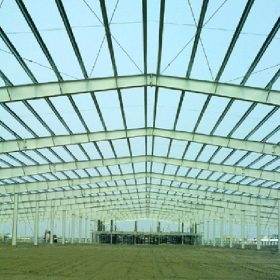
\includegraphics[width=64mm,height=64mm]{../../public/project-assets/sumidenso.jpg}};
    \fill[TTCDeepNavy,opacity=.88] (0,155) rectangle (64,166);
    \node[anchor=west,text=white,font=\fontsize{6.8}{8}\selectfont\bfseries]
      at (4,160.5) {ẢNH KHU NHÀ XƯỞNG};
  \end{scope}
  \draw[TTCBorder,rounded corners=4pt,line width=.7pt] (0,155) rectangle (64,219);

  \fill[TTCLightBlue,rounded corners=4pt] (68,155) rectangle (186,219);
  \draw[TTCBorder,rounded corners=4pt,line width=.7pt] (68,155) rectangle (186,219);
  \node[anchor=north west,text=TTCBlue,font=\fontsize{8}{9.5}\selectfont\bfseries]
    at (75,212) {HỒ SƠ DỰ ÁN};
  \node[anchor=north west,text width=48mm,text=TTCTextDark,font=\fontsize{7.1}{8.8}\selectfont]
    at (75,201) {\textbf{Chủ đầu tư:} Sumitomo Electric\\
                  \textbf{Quy mô:} 15.015 m$^2$\\
                  \textbf{Tiến độ:} 150 ngày};
  \draw[TTCBorder] (129,161) -- (129,208);
  \node[anchor=north west,text=TTCBlue,font=\fontsize{8}{9.5}\selectfont\bfseries]
    at (136,212) {TRỌNG TÂM BÀN GIAO};
  \node[anchor=north west,text width=43mm,text=TTCTextDark,font=\fontsize{6.9}{8.5}\selectfont]
    at (136,201) {\textbullet\quad Sprinkler phản ứng nhanh\\[1mm]
                  \textbullet\quad Trạm xử lý nước thải\\[1mm]
                  \textbullet\quad Kiểm soát hồ sơ theo chuẩn quản lý Nhật Bản};

  % Quality gates
  \node[anchor=west,text=TTCBlue,font=\fontsize{8}{9.5}\selectfont\bfseries]
    at (0,147) {BỐN CỔNG KIỂM SOÁT • CHỈ CHUYỂN BƯỚC KHI ĐỦ BẰNG CHỨNG};
  \fill[white,rounded corners=4pt] (0,88) rectangle (186,141);
  \draw[TTCBorder,rounded corners=4pt,line width=.7pt] (0,88) rectangle (186,141);
  \draw[TTCBlue,line width=.8pt] (23,122) -- (163,122);

  \foreach \x/\n in {23/01,69/02,117/03,163/04}{
    \fill[white] (\x,122) circle (6mm);
    \draw[TTCBlue,line width=.9pt] (\x,122) circle (6mm);
    \node[text=TTCBlue,font=\fontsize{7}{8}\selectfont\bfseries] at (\x,122) {\n};
  }
  \fill[TTCRed] (23,122) circle (3.2mm);
  \node[text=white,font=\fontsize{6.2}{7}\selectfont\bfseries] at (23,122) {01};

  \node[align=center,text width=38mm] at (23,101) {
    {\fontsize{7.3}{8.5}\selectfont\bfseries\color{TTCBlue}VẬT LIỆU ĐẦU VÀO}\\[-.3mm]
    {\fontsize{5.9}{7.1}\selectfont\color{TTCTextMuted}CO/CQ • mẫu duyệt • truy xuất lô}};
  \node[align=center,text width=38mm] at (69,101) {
    {\fontsize{7.3}{8.5}\selectfont\bfseries\color{TTCBlue}THI CÔNG / ITP}\\[-.3mm]
    {\fontsize{5.9}{7.1}\selectfont\color{TTCTextMuted}Checklist • hold point • nghiệm thu}};
  \node[align=center,text width=38mm] at (117,101) {
    {\fontsize{7.3}{8.5}\selectfont\bfseries\color{TTCBlue}CHẠY THỬ HỆ THỐNG}\\[-.3mm]
    {\fontsize{5.9}{7.1}\selectfont\color{TTCTextMuted}PCCC • xử lý nước thải • liên động}};
  \node[align=center,text width=38mm] at (163,101) {
    {\fontsize{7.3}{8.5}\selectfont\bfseries\color{TTCBlue}HỒ SƠ HOÀN CÔNG}\\[-.3mm]
    {\fontsize{5.9}{7.1}\selectfont\color{TTCTextMuted}As-built • biên bản • hướng dẫn O\&M}};

  % Ma trận yêu cầu -- kiểm soát -- bằng chứng
  \node[anchor=west,text=TTCBlue,font=\fontsize{8}{9.5}\selectfont\bfseries]
    at (0,80) {TỪ YÊU CẦU ĐẾN HỒ SƠ BÀN GIAO};
  \fill[TTCDeepNavy,rounded corners=3pt] (0,62) rectangle (186,75);
  \node[anchor=west,text=white,font=\fontsize{6.5}{7.8}\selectfont\bfseries] at (6,68.5) {HẠNG MỤC};
  \node[anchor=west,text=white,font=\fontsize{6.5}{7.8}\selectfont\bfseries] at (55,68.5) {ĐIỂM KIỂM SOÁT};
  \node[anchor=west,text=white,font=\fontsize{6.5}{7.8}\selectfont\bfseries] at (126,68.5) {BẰNG CHỨNG BÀN GIAO};

  \fill[TTCLightBlue] (0,47) rectangle (186,62);
  \fill[white] (0,32) rectangle (186,47);
  \fill[TTCLightBlue] (0,17) rectangle (186,32);
  \draw[TTCBorder] (49,17) -- (49,75);
  \draw[TTCBorder] (120,17) -- (120,75);
  \foreach \y in {17,32,47,62}{\draw[TTCBorder] (0,\y) -- (186,\y);}
  \node[anchor=west,text=TTCBlue,font=\fontsize{6.6}{8}\selectfont\bfseries] at (6,54.5) {PCCC SPRINKLER};
  \node[anchor=west,text=TTCTextDark,font=\fontsize{6.4}{7.8}\selectfont] at (55,54.5) {Áp lực • lưu lượng • liên động};
  \node[anchor=west,text=TTCTextDark,font=\fontsize{6.4}{7.8}\selectfont] at (126,54.5) {Biên bản thử và chứng từ thiết bị};
  \node[anchor=west,text=TTCBlue,font=\fontsize{6.6}{8}\selectfont\bfseries] at (6,39.5) {NƯỚC THẢI};
  \node[anchor=west,text=TTCTextDark,font=\fontsize{6.4}{7.8}\selectfont] at (55,39.5) {Vận hành thử • mẫu đầu ra};
  \node[anchor=west,text=TTCTextDark,font=\fontsize{6.4}{7.8}\selectfont] at (126,39.5) {Kết quả thử theo yêu cầu QCVN};
  \node[anchor=west,text=TTCBlue,font=\fontsize{6.6}{8}\selectfont\bfseries] at (6,24.5) {HOÀN THIỆN};
  \node[anchor=west,text=TTCTextDark,font=\fontsize{6.4}{7.8}\selectfont] at (55,24.5) {Mẫu duyệt • punch list • vệ sinh};
  \node[anchor=west,text=TTCTextDark,font=\fontsize{6.4}{7.8}\selectfont] at (126,24.5) {Checklist đóng việc và ảnh nghiệm thu};

  \fill[TTCDeepNavy,rounded corners=3pt] (0,0) rectangle (186,11);
  \node[anchor=west,text=white,font=\fontsize{7}{8.5}\selectfont\bfseries]
    at (7,5.5) {15.015 m$^2$};
  \node[text=white!35!gray] at (49,5.5) {|};
  \node[anchor=west,text=white,font=\fontsize{7}{8.5}\selectfont\bfseries]
    at (57,5.5) {150 NGÀY};
  \node[text=white!35!gray] at (95,5.5) {|};
  \node[anchor=west,text=white,font=\fontsize{7}{8.5}\selectfont\bfseries]
    at (103,5.5) {HỆ THỐNG PCCC + XỬ LÝ NƯỚC THẢI};
\end{tikzpicture}
\end{minipage}
\newpage

% ============================================================
% TRANG 27: PROJECT SPOTLIGHT -- XƯỞNG SẢN XUẤT FOXCONN
% ============================================================
\noindent\mbox{}\par\vspace{-\baselineskip}
\casepagebars{NHÀ XƯỞNG ĐIỆN TỬ • FOXCONN}{Trang 27}

\begin{minipage}[t][246mm]{\textwidth}
\secbrand{Hồ Sơ Dự Án 06: Xưởng Sản Xuất Foxconn}{Electronics manufacturing facility • KCN Quế Võ, Bắc Ninh}

\noindent
\begin{tikzpicture}[x=1mm,y=1mm]
  \path[use as bounding box] (0,0) rectangle (186,220);

  % Hero ngang, dùng đúng ảnh Foxconn
  \begin{scope}
    \clip[rounded corners=4pt] (0,151) rectangle (186,219);
    \node[inner sep=0pt] at (93,185)
      {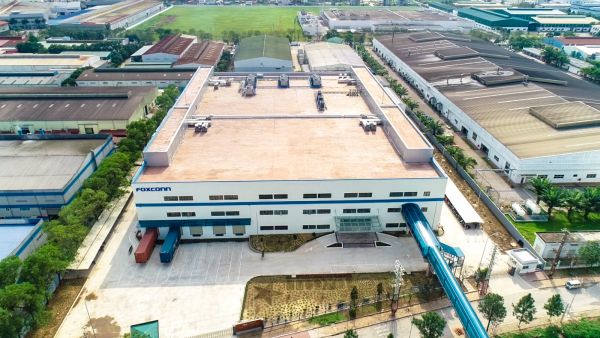
\includegraphics[width=186mm]{../../public/project-assets/foxcon.png}};
    \fill[TTCDeepNavy,opacity=.9] (0,151) rectangle (78,168);
    \node[anchor=west,text=white,font=\fontsize{7}{8}\selectfont\bfseries]
      at (5,159.5) {ẢNH DỰ ÁN • KCN QUẾ VÕ, BẮC NINH};
    \fill[TTCDeepNavy,opacity=.92] (127,151) rectangle (186,219);
    \node[anchor=north west,text=TTCCyan,font=\fontsize{6.8}{8}\selectfont\bfseries]
      at (133,212) {THÔNG TIN DỰ ÁN};
    \node[anchor=north west,text=white,font=\fontsize{14}{15}\selectfont\bfseries]
      at (133,201) {12.000 m$^2$};
    \node[anchor=north west,text=white!70!gray,font=\fontsize{6}{7.2}\selectfont]
      at (133,187) {DIỆN TÍCH NHÀ XƯỞNG};
    \draw[white!25!gray] (133,181) -- (180,181);
    \node[anchor=north west,text width=43mm,text=white,font=\fontsize{6.5}{8}\selectfont]
      at (133,177) {\textbf{Chủ đầu tư:} Foxconn\\
                    \textbf{Quốc gia:} Đài Loan\\
                    \textbf{Vai trò TTC:} Kết cấu thép và lắp dựng};
  \end{scope}
  \draw[TTCBorder,rounded corners=4pt,line width=.7pt] (0,151) rectangle (186,219);

  % Luồng triển khai theo zone -- hình thức khác 5 trang trước
  \node[anchor=west,text=TTCBlue,font=\fontsize{8}{9.5}\selectfont\bfseries]
    at (0,143) {LUỒNG TRIỂN KHAI • KHÓA GIAO DIỆN TRƯỚC KHI LẮP DỰNG};
  \fill[TTCLightBlue,rounded corners=4pt] (0,68) rectangle (186,137);
  \draw[TTCBorder,rounded corners=4pt,line width=.7pt] (0,68) rectangle (186,137);

  % Bốn thẻ quy trình độc lập; mũi tên chỉ nằm trong khe giữa các thẻ
  \foreach \xa/\xb in {4/43,50/89,96/135,142/182}{
    \fill[white,rounded corners=3pt] (\xa,74) rectangle (\xb,132);
    \draw[TTCBorder,rounded corners=3pt,line width=.65pt] (\xa,74) rectangle (\xb,132);
    \draw[TTCBlue,line width=1.2pt] ({\xa+4},128) -- ({\xb-4},128);
  }
  \foreach \xa/\xb in {43/50,89/96,135/142}{
    \draw[-{Latex[length=2mm]},TTCBlue!65!white,line width=.8pt]
      ({\xa+1},103) -- ({\xb-1},103);
  }

  \fill[TTCRed] (10,122) circle (3.5mm);
  \node[text=white,font=\fontsize{6}{7}\selectfont\bfseries] at (10,122) {01};
  \node[anchor=north west,text width=29mm,align=left,text=TTCBlue,
        font=\fontsize{7.2}{8.5}\selectfont\bfseries]
    at (9,115) {PHỐI HỢP\\THIẾT KẾ};
  \node[anchor=north west,text width=29mm,align=left,text=TTCTextMuted,
        font=\fontsize{6.1}{7.4}\selectfont]
    at (9,96) {Chốt trục, cao độ và giao diện kết cấu--MEP.};

  \fill[TTCBlue] (56,122) circle (3.5mm);
  \node[text=white,font=\fontsize{6}{7}\selectfont\bfseries] at (56,122) {02};
  \node[anchor=north west,text width=29mm,align=left,text=TTCBlue,
        font=\fontsize{7.2}{8.5}\selectfont\bfseries]
    at (55,115) {SẢN XUẤT\\CẤU KIỆN};
  \node[anchor=north west,text width=29mm,align=left,text=TTCTextMuted,
        font=\fontsize{6.1}{7.4}\selectfont]
    at (55,96) {Kiểm soát vật liệu, kích thước và liên kết tại xưởng.};

  \fill[TTCBlue] (102,122) circle (3.5mm);
  \node[text=white,font=\fontsize{6}{7}\selectfont\bfseries] at (102,122) {03};
  \node[anchor=north west,text width=29mm,align=left,text=TTCBlue,
        font=\fontsize{7.2}{8.5}\selectfont\bfseries]
    at (101,115) {LẮP DỰNG\\THEO ZONE};
  \node[anchor=north west,text width=29mm,align=left,text=TTCTextMuted,
        font=\fontsize{6.1}{7.4}\selectfont]
    at (101,96) {Ổn định khung và mở mặt bằng cuốn chiếu.};

  \fill[TTCBlue] (148,122) circle (3.5mm);
  \node[text=white,font=\fontsize{6}{7}\selectfont\bfseries] at (148,122) {04};
  \node[anchor=north west,text width=29mm,align=left,text=TTCBlue,
        font=\fontsize{7.2}{8.5}\selectfont\bfseries]
    at (147,115) {NGHIỆM THU\\CHUYỂN BƯỚC};
  \node[anchor=north west,text width=29mm,align=left,text=TTCTextMuted,
        font=\fontsize{6.1}{7.4}\selectfont]
    at (147,96) {Kiểm tra hình học, liên kết và hồ sơ trước bao che.};

  % Hai khối nội dung cô đọng
  \fill[white,rounded corners=4pt] (0,19) rectangle (90,60);
  \draw[TTCBorder,rounded corners=4pt] (0,19) rectangle (90,60);
  \node[anchor=north west,text=TTCRed,font=\fontsize{8}{9}\selectfont\bfseries]
    at (6,54) {BÀI TOÁN DỰ ÁN};
  \node[anchor=north west,text width=77mm,align=left,text=TTCTextDark,
        font=\fontsize{6.9}{8.5}\selectfont]
    at (6,44) {Nhà xưởng điện tử yêu cầu mặt bằng lớn, giao diện kết cấu--MEP rõ ràng và trình tự lắp dựng không làm gián đoạn các khu vực kế cận.};

  \fill[TTCLightBlue,rounded corners=4pt] (96,19) rectangle (186,60);
  \draw[TTCBorder,rounded corners=4pt] (96,19) rectangle (186,60);
  \node[anchor=north west,text=TTCBlue,font=\fontsize{8}{9}\selectfont\bfseries]
    at (102,54) {PHẢN HỒI CỦA TTC};
  \node[anchor=north west,text width=77mm,align=left,text=TTCTextDark,
        font=\fontsize{6.9}{8.5}\selectfont]
    at (102,44) {Chia zone thi công, kiểm soát cấu kiện từ xưởng và nghiệm thu từng bước để bàn giao mặt bằng theo trình tự rõ ràng.};

  \fill[TTCDeepNavy,rounded corners=3pt] (0,0) rectangle (186,12);
  \node[anchor=west,text=TTCCyan,font=\fontsize{6.2}{7.4}\selectfont\bfseries]
    at (7,6) {NGUYÊN TẮC TRIỂN KHAI};
  \draw[white!28!gray] (47,3) -- (47,9);
  \node[anchor=west,text=white,font=\fontsize{7}{8.5}\selectfont\bfseries]
    at (54,6) {KHÓA GIAO DIỆN → CHIA ZONE → NGHIỆM THU CHUYỂN BƯỚC};
\end{tikzpicture}
\end{minipage}
\newpage

% ============================================================
% TRANG 28: CHUỖI CUNG ỨNG KIỂM SOÁT
% ============================================================
\noindent\mbox{}\par\vspace{-\baselineskip}
\casepagebars{CHUỖI CUNG ỨNG • KIỂM SOÁT VẬT TƯ}{Trang 28}

\begin{minipage}[t][246mm]{\textwidth}
\secbrand{Chuỗi Cung Ứng Được Kiểm Soát Theo Từng Lô}{Approved sources • Material submittal • CO/CQ/MTC • Lot traceability}

\noindent
\begin{tikzpicture}[x=1mm,y=1mm]
  \path[use as bounding box] (0,0) rectangle (186,220);

  \node[anchor=west,text=TTCBlue,font=\fontsize{15}{17}\selectfont\bfseries]
    at (0,211) {VẬT TƯ CHỈ ĐƯỢC LẮP ĐẶT SAU KHI ĐỦ HỒ SƠ};
  \node[anchor=west,text=TTCTextMuted,font=\fontsize{7.2}{8.8}\selectfont]
    at (0,201) {Một luồng phê duyệt thống nhất giúp khóa chất lượng, nguồn gốc và khả năng thay thế trước khi mua hàng.};

  % Cột quy trình 4 cổng kiểm soát
  \fill[TTCDeepNavy,rounded corners=4pt] (0,79) rectangle (62,192);
  \node[anchor=west,text=TTCCyan,font=\fontsize{7}{8.3}\selectfont\bfseries]
    at (7,184) {4 CỔNG KIỂM SOÁT};
  \draw[white!18!gray] (7,178) -- (55,178);

  \foreach \y/\n/\title/\desc in {
    158/01/PHÊ DUYỆT NGUỒN/Nhà sản xuất • mẫu • dữ liệu kỹ thuật,
    134/02/KHÓA HỒ SƠ/CO--CQ • MTC • catalogue • bảo hành,
    110/03/KIỂM TRA ĐẦU VÀO/Nhãn lô • kích thước • tình trạng • thí nghiệm,
    88/04/TRUY XUẤT LẮP ĐẶT/Lô vật tư gắn với khu vực và biên bản nghiệm thu}
  {
    \fill[white,rounded corners=2pt] (7,{\y-8}) rectangle (55,{\y+8});
    \fill[TTCRed] (7,{\y-8}) rectangle (16,{\y+8});
    \node[text=white,font=\fontsize{6.2}{7}\selectfont\bfseries] at (11.5,\y) {\n};
    \node[anchor=north west,text width=34mm,text=TTCBlue,
          font=\fontsize{6.7}{7.8}\selectfont\bfseries] at (19,{\y+5}) {\title};
    \node[anchor=north west,text width=34mm,text=TTCTextMuted,
          font=\fontsize{5.6}{6.7}\selectfont] at (19,{\y-1}) {\desc};
  }

  % Ma trận nhóm vật tư
  \fill[white,rounded corners=4pt] (67,79) rectangle (186,192);
  \draw[TTCBorder,rounded corners=4pt,line width=.7pt] (67,79) rectangle (186,192);
  \node[anchor=west,text=TTCBlue,font=\fontsize{8}{9.4}\selectfont\bfseries]
    at (74,184) {NHÓM VẬT TƯ / THƯƠNG HIỆU THAM CHIẾU};
  \node[anchor=west,text=TTCTextMuted,font=\fontsize{5.8}{7}\selectfont]
    at (74,176) {Lựa chọn cuối cùng tuân theo hồ sơ phê duyệt vật liệu của từng dự án.};

  \foreach \y/\n/\name/\brands/\control in {
    157/01/THÉP \& BAO CHE/POSCO • Hòa Phát • BlueScope/MTC • mác thép • lớp mạ,
    134/02/SƠN \& HÓA CHẤT/Jotun • KCC • Sika/Batch • DFT • chứng nhận PCCC,
    111/03/ĐIỆN \& MEP/Schneider • ABB • LS Vina/Catalogue • test • xuất xứ,
    88/04/HVAC \& PCCC/Daikin • Grundfos • Tyco/Submittal • UL--FM khi yêu cầu}
  {
    \fill[TTCLightBlue,rounded corners=2pt] (73,{\y-9}) rectangle (180,{\y+9});
    \node[anchor=west,text=TTCRed,font=\fontsize{6.4}{7.5}\selectfont\bfseries]
      at (78,{\y+4}) {\n};
    \node[anchor=west,text=TTCBlue,font=\fontsize{7}{8.2}\selectfont\bfseries]
      at (91,{\y+4}) {\name};
    \node[anchor=west,text=TTCTextDark,font=\fontsize{6.2}{7.3}\selectfont]
      at (91,{\y-2}) {\brands};
    \node[anchor=east,text=TTCTextMuted,font=\fontsize{5.6}{6.7}\selectfont]
      at (176,{\y-7}) {Kiểm soát: \control};
  }

  % Ba lớp bảo chứng
  \node[anchor=west,text=TTCBlue,font=\fontsize{8}{9.4}\selectfont\bfseries]
    at (0,68) {BA LỚP BẢO CHỨNG TRƯỚC KHI LẮP ĐẶT};
  \foreach \xa/\xb/\n/\title/\desc in {
    0/58/01/ĐÚNG NGUỒN/Hồ sơ phê duyệt khớp nhà sản xuất và xuất xứ,
    64/122/02/ĐÚNG CHẤT LƯỢNG/Chỉ tiêu kỹ thuật khớp mẫu và tiêu chuẩn dự án,
    128/186/03/ĐÚNG VỊ TRÍ/Mỗi lô gắn với biên bản và khu vực sử dụng}
  {
    \fill[white,rounded corners=3pt] (\xa,25) rectangle (\xb,60);
    \draw[TTCBorder,rounded corners=3pt] (\xa,25) rectangle (\xb,60);
    \node[anchor=west,text=TTCRed,font=\fontsize{7}{8}\selectfont\bfseries]
      at ({\xa+6},52) {\n};
    \node[anchor=west,text=TTCBlue,font=\fontsize{7.4}{8.7}\selectfont\bfseries]
      at ({\xa+17},52) {\title};
    \node[anchor=north west,text width=46mm,text=TTCTextMuted,
          font=\fontsize{6.2}{7.5}\selectfont] at ({\xa+6},43) {\desc};
  }

  \fill[TTCDeepNavy,rounded corners=3pt] (0,0) rectangle (186,16);
  \node[anchor=west,text=TTCCyan,font=\fontsize{6.3}{7.5}\selectfont\bfseries]
    at (7,8) {MATERIAL ASSURANCE};
  \node[anchor=east,text=white,font=\fontsize{7.2}{8.5}\selectfont\bfseries]
    at (179,8) {APPROVED SOURCE → VERIFIED LOT → TRACEABLE INSTALLATION};
\end{tikzpicture}
\end{minipage}
\newpage

% ============================================================
% TRANG 29: HỆ SINH THÁI CÔNG TRÌNH THEO NGÀNH
% ============================================================
\noindent\mbox{}\par\vspace{-\baselineskip}
\casepagebars{HỆ SINH THÁI DỰ ÁN • 6 NHÓM NGÀNH}{Trang 29}

\begin{minipage}[t][246mm]{\textwidth}
\secbrand{Sáu Hệ Công Trình — Một Năng Lực Tích Hợp}{Representative sectors • Different operating demands • One coordinated EPC workflow}

\noindent
\begin{tikzpicture}[x=1mm,y=1mm]
  \path[use as bounding box] (0,0) rectangle (186,220);
  \node[anchor=west,text=TTCBlue,font=\fontsize{15}{17}\selectfont\bfseries]
    at (0,211) {THIẾT KẾ BẮT ĐẦU TỪ CÁCH NHÀ MÁY VẬN HÀNH};
  \node[anchor=west,text=TTCTextMuted,font=\fontsize{7.2}{8.8}\selectfont]
    at (0,201) {Mỗi nhóm ngành có một rủi ro cốt lõi; giải pháp kết cấu, MEP và trình tự thi công phải trả lời đúng rủi ro đó.};

  % Hàng 1
  \begin{scope}
    \clip[rounded corners=3pt] (0,132) rectangle (59,190);
    \node[inner sep=0pt] at (29.5,165) {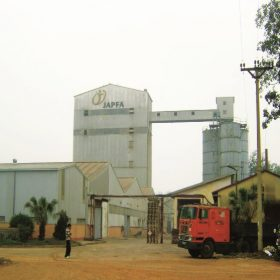
\includegraphics[width=60mm]{../../public/project-assets/japfa.jpg}};
    \fill[TTCDeepNavy,opacity=.9] (0,132) rectangle (59,151);
  \end{scope}
  \draw[TTCBorder,rounded corners=3pt] (0,132) rectangle (59,190);
  \node[anchor=west,text=white,font=\fontsize{7.5}{8.8}\selectfont\bfseries] at (5,144) {THỰC PHẨM \& AGRIFOOD};
  \node[anchor=west,text=white!75!gray,font=\fontsize{5.8}{7}\selectfont] at (5,137) {Silo • process • vệ sinh • PCCC};

  \begin{scope}
    \clip[rounded corners=3pt] (63.5,132) rectangle (122.5,190);
    \node[inner sep=0pt] at (93,167) {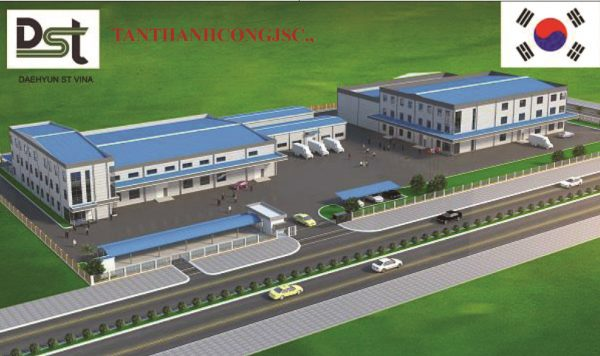
\includegraphics[height=41mm]{../../public/project-assets/daeyun.jpg}};
    \fill[TTCDeepNavy,opacity=.9] (63.5,132) rectangle (122.5,151);
  \end{scope}
  \draw[TTCBorder,rounded corners=3pt] (63.5,132) rectangle (122.5,190);
  \node[anchor=west,text=white,font=\fontsize{7.5}{8.8}\selectfont\bfseries] at (68.5,144) {ĐIỆN TỬ \& PHÒNG SẠCH};
  \node[anchor=west,text=white!75!gray,font=\fontsize{5.8}{7}\selectfont] at (68.5,137) {HVAC • ESD • kiểm soát môi trường};

  \begin{scope}
    \clip[rounded corners=3pt] (127,132) rectangle (186,190);
    \node[inner sep=0pt] at (156.5,168) {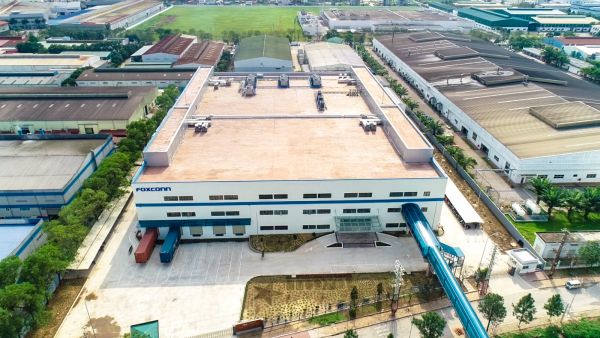
\includegraphics[height=41mm]{../../public/project-assets/foxcon.png}};
    \fill[TTCDeepNavy,opacity=.9] (127,132) rectangle (186,151);
  \end{scope}
  \draw[TTCBorder,rounded corners=3pt] (127,132) rectangle (186,190);
  \node[anchor=west,text=white,font=\fontsize{7.5}{8.8}\selectfont\bfseries] at (132,144) {NHÀ XƯỞNG ĐIỆN TỬ};
  \node[anchor=west,text=white!75!gray,font=\fontsize{5.8}{7}\selectfont] at (132,137) {Giao diện MEP • lắp dựng theo zone};

  % Hàng 2
  \begin{scope}
    \clip[rounded corners=3pt] (0,69) rectangle (59,127);
    \node[inner sep=0pt] at (29.5,103) {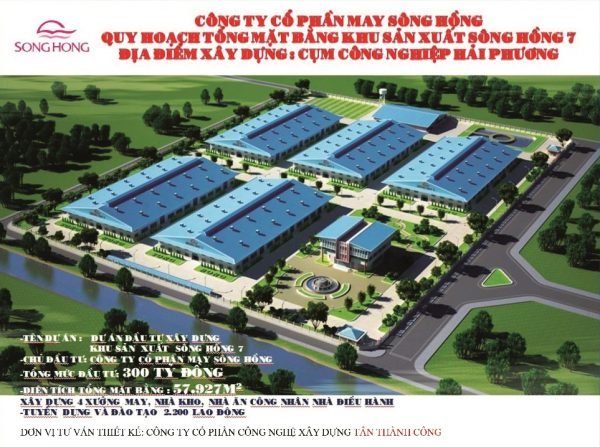
\includegraphics[height=42mm]{../../public/project-assets/songhong7.jpg}};
    \fill[TTCDeepNavy,opacity=.9] (0,69) rectangle (59,88);
  \end{scope}
  \draw[TTCBorder,rounded corners=3pt] (0,69) rectangle (59,127);
  \node[anchor=west,text=white,font=\fontsize{7.5}{8.8}\selectfont\bfseries] at (5,81) {DỆT MAY NHIỀU TẦNG};
  \node[anchor=west,text=white!75!gray,font=\fontsize{5.8}{7}\selectfont] at (5,74) {Sàn tải nặng • nhịp lớn • thoát nạn};

  \begin{scope}
    \clip[rounded corners=3pt] (63.5,69) rectangle (122.5,127);
    \node[inner sep=0pt] at (93,104) {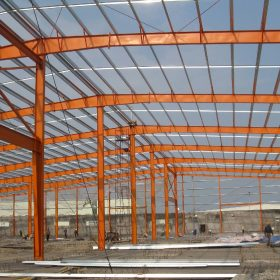
\includegraphics[width=60mm]{../../public/project-assets/yusen.jpg}};
    \fill[TTCDeepNavy,opacity=.9] (63.5,69) rectangle (122.5,88);
  \end{scope}
  \draw[TTCBorder,rounded corners=3pt] (63.5,69) rectangle (122.5,127);
  \node[anchor=west,text=white,font=\fontsize{7.5}{8.8}\selectfont\bfseries] at (68.5,81) {LOGISTICS \& KHO VẬN};
  \node[anchor=west,text=white!75!gray,font=\fontsize{5.8}{7}\selectfont] at (68.5,74) {Sàn phẳng • dock • luồng xe hàng};

  \begin{scope}
    \clip[rounded corners=3pt] (127,69) rectangle (186,127);
    \node[inner sep=0pt] at (156.5,104) {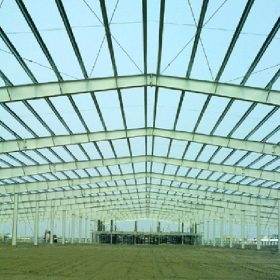
\includegraphics[width=60mm]{../../public/project-assets/sumidenso.jpg}};
    \fill[TTCDeepNavy,opacity=.9] (127,69) rectangle (186,88);
  \end{scope}
  \draw[TTCBorder,rounded corners=3pt] (127,69) rectangle (186,127);
  \node[anchor=west,text=white,font=\fontsize{7.5}{8.8}\selectfont\bfseries] at (132,81) {LINH KIỆN Ô TÔ};
  \node[anchor=west,text=white!75!gray,font=\fontsize{5.8}{7}\selectfont] at (132,74) {Chất lượng ổn định • bàn giao theo gate};

  % Ba năng lực dùng chung
  \node[anchor=west,text=TTCBlue,font=\fontsize{8}{9.3}\selectfont\bfseries]
    at (0,58) {NĂNG LỰC XUYÊN SUỐT MỌI NHÓM NGÀNH};
  \foreach \xa/\xb/\title/\desc in {
    0/58/COORDINATION/Khóa giao diện kiến trúc • kết cấu • MEP,
    64/122/CONSTRUCTABILITY/Thiết kế bám biện pháp và trình tự thi công,
    128/186/HANDOVER/Đủ bằng chứng trước mỗi bước chuyển giao}
  {
    \fill[TTCLightBlue,rounded corners=3pt] (\xa,20) rectangle (\xb,50);
    \node[anchor=west,text=TTCBlue,font=\fontsize{7.2}{8.5}\selectfont\bfseries]
      at ({\xa+6},41) {\title};
    \node[anchor=north west,text width=46mm,text=TTCTextMuted,
          font=\fontsize{6.1}{7.3}\selectfont] at ({\xa+6},34) {\desc};
  }
  \fill[TTCDeepNavy,rounded corners=3pt] (0,0) rectangle (186,12);
  \node[anchor=west,text=TTCCyan,font=\fontsize{6.2}{7.4}\selectfont\bfseries] at (7,6) {SECTOR FIT};
  \node[anchor=east,text=white,font=\fontsize{7}{8.3}\selectfont\bfseries]
    at (179,6) {GIẢI PHÁP ĐƯỢC THIẾT KẾ THEO NHU CẦU VẬN HÀNH};
\end{tikzpicture}
\end{minipage}
\newpage

% ============================================================
% TRANG 30: BỘ HỒ SƠ BÀN GIAO
% ============================================================
\noindent\mbox{}\par\vspace{-\baselineskip}
\casepagebars{BẰNG CHỨNG BÀN GIAO • CLOSEOUT DOSSIER}{Trang 30}

\begin{minipage}[t][246mm]{\textwidth}
\secbrand{Bộ Hồ Sơ Bàn Giao Có Thể Truy Xuất}{Evidence chain from approved material to as-built and commissioning records}

\noindent
\begin{tikzpicture}[x=1mm,y=1mm]
  \path[use as bounding box] (0,0) rectangle (186,220);
  \node[anchor=west,text=TTCBlue,font=\fontsize{15}{17}\selectfont\bfseries]
    at (0,211) {BÀN GIAO CÔNG TRÌNH — ĐỒNG THỜI BÀN GIAO BẰNG CHỨNG};
  \node[anchor=west,text=TTCTextMuted,font=\fontsize{7.2}{8.8}\selectfont]
    at (0,201) {Mỗi bước chỉ được đóng khi hồ sơ kỹ thuật, biên bản và bằng chứng hiện trường đã khớp nhau.};

  % Dòng 5 cổng bằng chứng
  \fill[TTCLightBlue,rounded corners=4pt] (0,139) rectangle (186,190);
  \draw[TTCBorder,rounded corners=4pt] (0,139) rectangle (186,190);
  \draw[TTCBlue!40!white,line width=.8pt] (18,165) -- (168,165);
  \foreach \x/\n/\title in {
    18/01/VẬT TƯ,
    55.5/02/SHOP DRAWING,
    93/03/NGHIỆM THU,
    130.5/04/AS-BUILT,
    168/05/COMMISSIONING}
  {
    \fill[white] (\x,165) circle (5mm);
    \draw[TTCBlue,line width=.8pt] (\x,165) circle (5mm);
    \node[text=TTCBlue,font=\fontsize{6}{7}\selectfont\bfseries] at (\x,165) {\n};
    \node[anchor=north,align=center,text width=29mm,text=TTCBlue,
          font=\fontsize{6.5}{7.7}\selectfont\bfseries] at (\x,155) {\title};
  }
  \fill[TTCRed] (18,165) circle (3.5mm);
  \node[text=white,font=\fontsize{5.8}{6.8}\selectfont\bfseries] at (18,165) {01};

  % Minh họa tập hồ sơ
  \fill[TTCDeepNavy,rounded corners=4pt] (0,48) rectangle (70,130);
  \node[anchor=west,text=TTCCyan,font=\fontsize{7}{8.2}\selectfont\bfseries]
    at (7,121) {CLOSEOUT DOSSIER};
  \fill[white!15!gray,rounded corners=2pt] (15,61) rectangle (61,111);
  \fill[white!45!gray,rounded corners=2pt] (12,65) rectangle (58,115);
  \fill[white,rounded corners=2pt] (9,69) rectangle (55,119);
  \fill[TTCRed] (9,112) rectangle (55,119);
  \node[anchor=west,text=TTCBlue,font=\fontsize{7.4}{8.6}\selectfont\bfseries]
    at (15,103) {HỒ SƠ HOÀN CÔNG};
  \draw[TTCBorder] (15,96) -- (49,96);
  \draw[TTCBorder] (15,90) -- (49,90);
  \draw[TTCBorder] (15,84) -- (42,84);
  \node[anchor=west,text=TTCTextMuted,font=\fontsize{5.8}{7}\selectfont]
    at (15,76) {CDE index • revision • approval};
  \node[anchor=west,text=white,font=\fontsize{6.1}{7.3}\selectfont\bfseries]
    at (7,55) {01 BỘ CHỈ MỤC • NHIỀU NHÓM HỒ SƠ};

  % Checklist bên phải
  \fill[white,rounded corners=4pt] (76,48) rectangle (186,130);
  \draw[TTCBorder,rounded corners=4pt] (76,48) rectangle (186,130);
  \node[anchor=west,text=TTCBlue,font=\fontsize{8}{9.4}\selectfont\bfseries]
    at (83,120) {CẤU TRÚC BÀN GIAO TỐI THIỂU};
  \foreach \y/\n/\title/\desc in {
    104/01/HỒ SƠ VẬT LIỆU/Approved submittal • CO/CQ • MTC • test,
    90/02/HỒ SƠ THI CÔNG/ITP • checklist • biên bản nghiệm thu,
    76/03/HỒ SƠ HOÀN CÔNG/Bản vẽ as-built • revision • xác nhận,
    62/04/HỒ SƠ VẬN HÀNH/O\&M manual • bảo hành • danh mục thiết bị}
  {
    \fill[TTCLightBlue,rounded corners=2pt] (83,{\y-6}) rectangle (179,{\y+6});
    \node[anchor=west,text=TTCRed,font=\fontsize{6.2}{7.2}\selectfont\bfseries]
      at (88,\y) {\n};
    \node[anchor=west,text=TTCBlue,font=\fontsize{6.6}{7.7}\selectfont\bfseries]
      at (101,{\y+2}) {\title};
    \node[anchor=west,text=TTCTextMuted,font=\fontsize{5.6}{6.7}\selectfont]
      at (101,{\y-4}) {\desc};
  }

  % Nguyên tắc phát hành
  \node[anchor=west,text=TTCBlue,font=\fontsize{8}{9.3}\selectfont\bfseries]
    at (0,37) {NGUYÊN TẮC PHÁT HÀNH};
  \fill[TTCDeepNavy,rounded corners=3pt] (0,0) rectangle (186,29);
  \node[anchor=west,text=TTCCyan,font=\fontsize{6.2}{7.4}\selectfont\bfseries]
    at (7,20) {RELEASE CONTROL};
  \node[anchor=west,text=white,font=\fontsize{9}{10.5}\selectfont\bfseries]
    at (7,10) {ĐÃ KIỂM TRA → ĐỦ BẰNG CHỨNG → ĐÃ DUYỆT → TRUY XUẤT ĐƯỢC};
  \node[anchor=east,text=white!70!gray,font=\fontsize{6.1}{7.3}\selectfont]
    at (179,20) {Một phiên bản hiệu lực • Một chỉ mục bàn giao};
\end{tikzpicture}
\end{minipage}
\newpage

% ============================================================
% TRANG 31: NỀN TẢNG PHÁP LÝ VÀ HỆ QUẢN TRỊ
% ============================================================
\noindent\mbox{}\par\vspace{-\baselineskip}
\casepagebars{NỀN TẢNG PHÁP LÝ • HỆ QUẢN TRỊ}{Trang 31}

\begin{minipage}[t][246mm]{\textwidth}
\secbrand{Hồ Sơ Pháp Lý Sẵn Sàng Cho Thẩm Định}{Corporate identity • Construction capability • ISO systems • Key-person credentials}

\noindent
\begin{tikzpicture}[x=1mm,y=1mm]
  \path[use as bounding box] (0,0) rectangle (186,220);
  \node[anchor=west,text=TTCBlue,font=\fontsize{15}{17}\selectfont\bfseries]
    at (0,211) {MỘT BỘ HỒ SƠ — BỐN LỚP NĂNG LỰC CÓ THỂ ĐỐI CHIẾU};
  \node[anchor=west,text=TTCTextMuted,font=\fontsize{7.2}{8.8}\selectfont]
    at (0,201) {Thông tin pháp nhân, phạm vi hoạt động và hệ thống quản trị được tổ chức theo đúng logic của vòng thẩm định nhà thầu.};

  % Hồ sơ pháp nhân lớn bên trái
  \fill[TTCDeepNavy,rounded corners=4pt] (0,57) rectangle (67,191);
  \node[anchor=west,text=TTCCyan,font=\fontsize{7}{8.3}\selectfont\bfseries]
    at (7,182) {CORPORATE IDENTITY};
  \node[anchor=north west,text width=53mm,text=white,
        font=\fontsize{12}{14}\selectfont\bfseries]
    at (7,169) {CÔNG TY CỔ PHẦN\\CÔNG NGHỆ XÂY DỰNG\\TÂN THÀNH CÔNG};
  \draw[white!20!gray] (7,125) -- (60,125);
  \node[anchor=north west,text width=53mm,text=white!82!gray,
        font=\fontsize{6.5}{8.2}\selectfont]
    at (7,116) {\textbf{Tên viết tắt:} TTC JSC\\[2mm]
                 \textbf{Mã số thuế:} 0107090447\\[2mm]
                 \textbf{Trụ sở:} Hà Nội, Việt Nam\\[2mm]
                 \textbf{Lĩnh vực:} Tổng thầu công nghiệp, kết cấu thép, MEP và quản lý dự án};
  \fill[TTCRed,rounded corners=2pt] (7,67) rectangle (60,82);
  \node[text=white,font=\fontsize{7}{8.2}\selectfont\bfseries] at (33.5,74.5)
    {LEGAL • TRACEABLE • BID-READY};

  % Bốn lớp hồ sơ bên phải
  \foreach \y/\n/\title/\desc in {
    166/01/NĂNG LỰC HOẠT ĐỘNG XÂY DỰNG/Phạm vi công việc và cấp năng lực được đối chiếu trực tiếp theo chứng chỉ còn hiệu lực.,
    134/02/HỆ THỐNG QUẢN LÝ ISO/ISO 9001 • ISO 14001 • ISO 45001 được trình bày cùng phạm vi áp dụng và kỳ đánh giá.,
    102/03/NHÂN SỰ CHỦ CHỐT/Chứng chỉ hành nghề của Giám đốc dự án • Chỉ huy trưởng • chủ trì thiết kế.,
    70/04/HỒ SƠ THƯƠNG MẠI/Đăng ký doanh nghiệp • thuế • ngân hàng • bảo hiểm • biểu mẫu hồ sơ dự thầu.}
  {
    \fill[white,rounded corners=3pt] (73,{\y-13}) rectangle (186,{\y+13});
    \draw[TTCBorder,rounded corners=3pt] (73,{\y-13}) rectangle (186,{\y+13});
    \fill[TTCLightBlue,rounded corners=2pt] (79,{\y-7}) rectangle (94,{\y+7});
    \node[text=TTCRed,font=\fontsize{7}{8}\selectfont\bfseries] at (86.5,\y) {\n};
    \node[anchor=west,text=TTCBlue,font=\fontsize{7.2}{8.5}\selectfont\bfseries]
      at (101,{\y+5}) {\title};
    \node[anchor=north west,text width=76mm,text=TTCTextMuted,
          font=\fontsize{6.1}{7.4}\selectfont] at (101,{\y-1}) {\desc};
  }

  % Checklist hồ sơ thầu
  \node[anchor=west,text=TTCBlue,font=\fontsize{8}{9.3}\selectfont\bfseries]
    at (0,46) {BỘ CHỈ MỤC PHỤC VỤ PRE-QUALIFICATION / TENDER};
  \foreach \xa/\xb/\label in {
    0/34/PHÁP NHÂN,
    38/72/NĂNG LỰC,
    76/110/ISO,
    114/148/NHÂN SỰ,
    152/186/TÀI CHÍNH}
  {
    \fill[TTCLightBlue,rounded corners=2pt] (\xa,20) rectangle (\xb,38);
    \node[text=TTCBlue,font=\fontsize{6.6}{7.8}\selectfont\bfseries]
      at ({(\xa+\xb)/2},29) {\label};
  }
  \fill[TTCDeepNavy,rounded corners=3pt] (0,0) rectangle (186,12);
  \node[anchor=west,text=TTCCyan,font=\fontsize{6.2}{7.4}\selectfont\bfseries] at (7,6) {DUE DILIGENCE};
  \node[anchor=east,text=white,font=\fontsize{7}{8.3}\selectfont\bfseries]
    at (179,6) {THÔNG TIN CÓ CHỈ MỤC • BẢN SAO CÓ KIỂM SOÁT • DỄ ĐỐI CHIẾU};
\end{tikzpicture}
\end{minipage}
\newpage

% ============================================================
% TRANG 32: BẢN ĐỒ HIỆN DIỆN DỰ ÁN
% ============================================================
\noindent\mbox{}\par\vspace{-\baselineskip}
\casepagebars{BẢN ĐỒ HIỆN DIỆN • CỤM CÔNG NGHIỆP}{Trang 32}

\begin{minipage}[t][246mm]{\textwidth}
\secbrand{Hiện Diện Theo Các Hành Lang Công Nghiệp Trọng Điểm}{Northern manufacturing belt • Central corridor • Southern FDI and logistics cluster}

\noindent
\begin{tikzpicture}[x=1mm,y=1mm]
  \path[use as bounding box] (0,0) rectangle (186,220);
  \node[anchor=west,text=TTCBlue,font=\fontsize{15}{17}\selectfont\bfseries]
    at (0,211) {BẢN ĐỒ KINH NGHIỆM TRIỂN KHAI TẠI VIỆT NAM};
  \node[anchor=west,text=TTCTextMuted,font=\fontsize{7.2}{8.8}\selectfont]
    at (0,201) {Các điểm nhấn phản ánh cụm địa bàn xuất hiện trong danh mục dự án; không biểu diễn số lượng dự án theo tỷ lệ.};

  % Khung bản đồ
  \fill[white,rounded corners=4pt] (0,24) rectangle (103,191);
  \draw[TTCBorder,rounded corners=4pt,line width=.7pt] (0,24) rectangle (103,191);
  \node[inner sep=0pt] at (51.5,107.5)
    {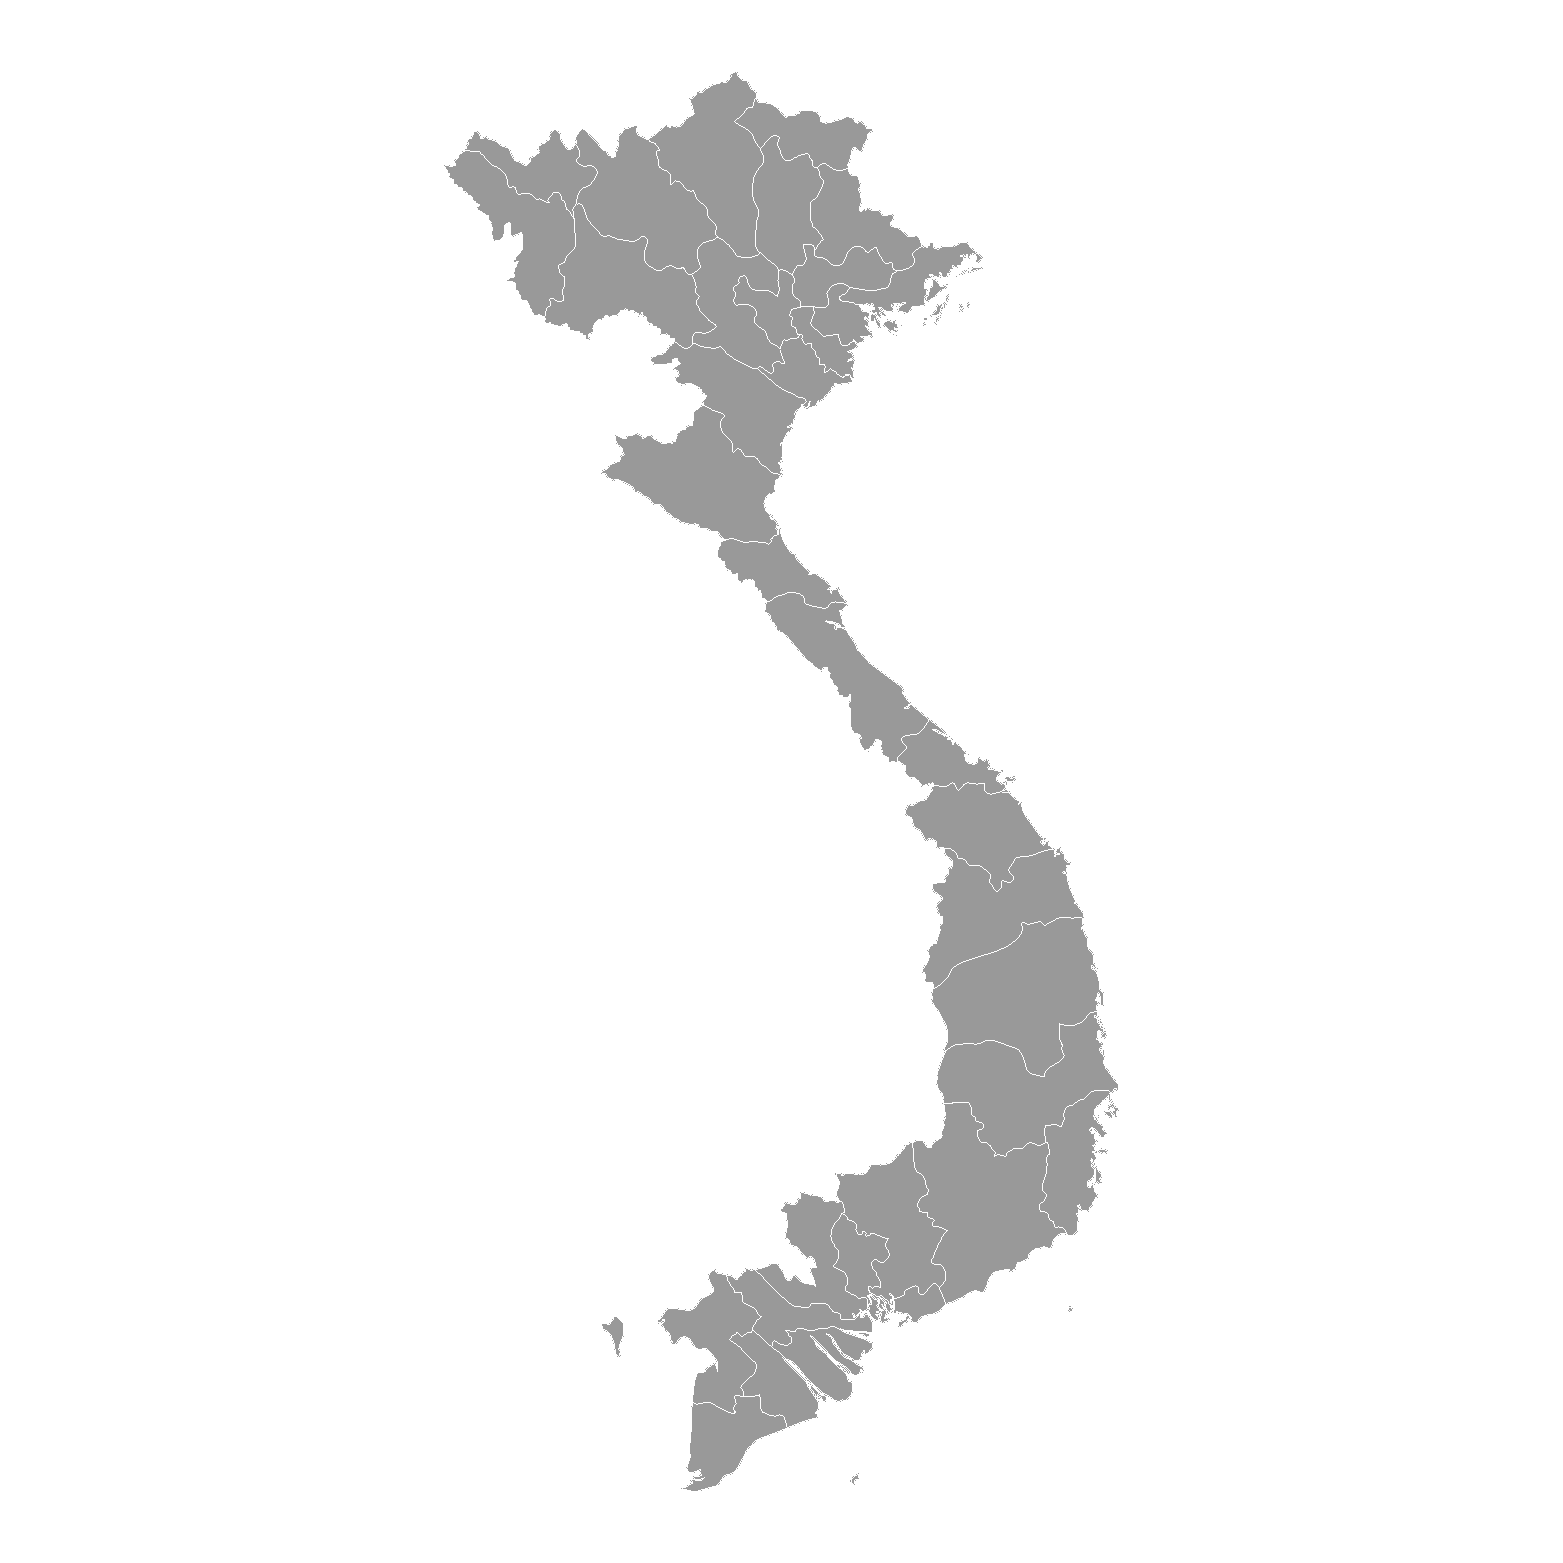
\includegraphics[height=164mm,trim=150 10 150 10,clip]{../../public/project-assets/vietnam-provinces.pdf}};

  % Highlight các cụm, vị trí chỉ báo gần đúng trên bản đồ nền
  \fill[TTCRed,opacity=.16] (62,151) circle (12mm);
  \draw[TTCRed,line width=1pt] (62,151) circle (6mm);
  \fill[TTCRed] (62,151) circle (2.2mm);
  \node[anchor=west,text=TTCRed,font=\fontsize{6.5}{7.6}\selectfont\bfseries] at (70,157) {CỤM BẮC BỘ};
  \node[anchor=west,text=TTCTextMuted,font=\fontsize{5.5}{6.6}\selectfont] at (70,150) {Hà Nội • Vĩnh Phúc • Bắc Ninh};

  \fill[TTCBlue,opacity=.14] (62,94) circle (10mm);
  \draw[TTCBlue,line width=1pt] (62,94) circle (5mm);
  \fill[TTCBlue] (62,94) circle (2mm);
  \node[anchor=west,text=TTCBlue,font=\fontsize{6.5}{7.6}\selectfont\bfseries] at (69,100) {HÀNH LANG MIỀN TRUNG};
  \node[anchor=west,text=TTCTextMuted,font=\fontsize{5.5}{6.6}\selectfont] at (69,93) {Đà Nẵng • Quảng Nam • duyên hải};

  \fill[TTCCyan,opacity=.16] (51,51) circle (10mm);
  \draw[TTCCyan,line width=1pt] (51,51) circle (5mm);
  \fill[TTCCyan] (51,51) circle (2mm);
  \node[anchor=west,text=TTCBlue,font=\fontsize{6.5}{7.6}\selectfont\bfseries] at (59,57) {CỤM PHÍA NAM};
  \node[anchor=west,text=TTCTextMuted,font=\fontsize{5.5}{6.6}\selectfont] at (59,50) {Bình Dương • TP.HCM • Hậu Giang};
  \node[anchor=west,text=TTCTextMuted,font=\fontsize{4.8}{5.8}\selectfont]
    at (5,29) {Bản đồ nền CC0: Wikimedia Commons / Thomson Walt};

  % Ba cụm thông tin bên phải
  \fill[TTCDeepNavy,rounded corners=4pt] (109,133) rectangle (186,191);
  \node[anchor=west,text=TTCCyan,font=\fontsize{6.2}{7.4}\selectfont\bfseries]
    at (116,183) {01 • TRỌNG TÂM HIỆN TẠI};
  \node[anchor=north west,text width=62mm,text=white,
        font=\fontsize{9.5}{11}\selectfont\bfseries] at (116,173) {VÀNH ĐAI CÔNG NGHIỆP BẮC BỘ};
  \node[anchor=north west,text width=62mm,text=white!75!gray,
        font=\fontsize{6.2}{7.6}\selectfont] at (116,153) {Mật độ dự án cao quanh các KCN Hà Nội, Vĩnh Phúc, Bắc Ninh, Bắc Giang, Hải Dương, Hải Phòng và Nam Định.};

  \fill[TTCLightBlue,rounded corners=4pt] (109,73) rectangle (186,127);
  \node[anchor=west,text=TTCRed,font=\fontsize{6.2}{7.4}\selectfont\bfseries]
    at (116,119) {02 • NĂNG LỰC CƠ ĐỘNG};
  \node[anchor=north west,text width=62mm,text=TTCBlue,
        font=\fontsize{8.5}{10}\selectfont\bfseries] at (116,109) {ĐỘI NGŨ THEO CỤM DỰ ÁN};
  \node[anchor=north west,text width=62mm,text=TTCTextMuted,
        font=\fontsize{6.2}{7.6}\selectfont] at (116,92) {Bố trí quản lý dự án, QA/QC và HSE theo địa bàn; kế hoạch huy động thiết bị được khóa theo từng gói công việc.};

  \fill[white,rounded corners=4pt] (109,24) rectangle (186,67);
  \draw[TTCBorder,rounded corners=4pt] (109,24) rectangle (186,67);
  \node[anchor=west,text=TTCBlue,font=\fontsize{6.2}{7.4}\selectfont\bfseries]
    at (116,59) {03 • HƯỚNG MỞ RỘNG};
  \node[anchor=north west,text width=62mm,text=TTCTextDark,
        font=\fontsize{6.3}{7.7}\selectfont] at (116,49) {Mở rộng có chọn lọc tại miền Trung và phía Nam, ưu tiên dự án có yêu cầu EPC công nghiệp, logistics và nhà máy công nghệ cao.};

  \fill[TTCDeepNavy,rounded corners=3pt] (109,0) rectangle (186,16);
  \node[anchor=west,text=TTCCyan,font=\fontsize{6.1}{7.2}\selectfont\bfseries]
    at (116,8) {PROJECT FOOTPRINT};
  \node[anchor=east,text=white,font=\fontsize{6.5}{7.7}\selectfont\bfseries]
    at (179,8) {3 CỤM TRIỂN KHAI};
\end{tikzpicture}
\end{minipage}
\newpage

% ============================================================
% TRANG 33: LỘ TRÌNH 2026--2030
% ============================================================
\noindent\mbox{}\par\vspace{-\baselineskip}
\casepagebars{LỘ TRÌNH 2026--2030 • TĂNG TRƯỞNG CÓ KIỂM SOÁT}{Trang 33}

\begin{minipage}[t][246mm]{\textwidth}
\secbrand{Lộ Trình Tăng Trưởng Chọn Lọc Và Lành Mạnh}{Controlled growth • Repeat clients • High-tech capability • Positive cash discipline}

\noindent
\begin{tikzpicture}[x=1mm,y=1mm]
  \path[use as bounding box] (0,0) rectangle (186,220);
  \node[anchor=west,text=TTCBlue,font=\fontsize{15}{17}\selectfont\bfseries]
    at (0,211) {TĂNG QUY MÔ SAU KHI NĂNG LỰC QUẢN TRỊ ĐÃ SẴN SÀNG};
  \node[anchor=west,text=TTCTextMuted,font=\fontsize{7.2}{8.8}\selectfont]
    at (0,201) {Mục tiêu doanh thu được điều chỉnh thận trọng, đặt chất lượng dòng tiền và khả năng bàn giao lên trước tốc độ mở rộng.};

  % Ba horizon cards
  \foreach \xa/\xb/\year/\value/\focus/\desc in {
    0/58/2026/300--400 TỶ/CỦNG CỐ NỀN TẢNG/Chuẩn hóa CDE • kiểm soát chi phí • củng cố năng lực miền Bắc,
    64/122/2027--2028/THEO NĂNG LỰC/MỞ RỘNG CHỌN LỌC/Tăng dự án công nghệ cao • phòng sạch • khách hàng lặp lại,
    128/186/2029--2030/THEO DÒNG TIỀN/QUY MÔ BỀN VỮNG/Mở rộng địa bàn có điều kiện • ưu tiên tổng thầu giá trị cao}
  {
    \fill[white,rounded corners=4pt] (\xa,68) rectangle (\xb,190);
    \draw[TTCBorder,rounded corners=4pt,line width=.7pt] (\xa,68) rectangle (\xb,190);
    \fill[TTCDeepNavy,rounded corners=4pt] (\xa,165) rectangle (\xb,190);
    \node[anchor=west,text=TTCCyan,font=\fontsize{7}{8.3}\selectfont\bfseries]
      at ({\xa+6},181) {\year};
    \node[anchor=west,text=white,font=\fontsize{13}{15}\selectfont\bfseries]
      at ({\xa+6},171) {\value};
    \fill[TTCRed] ({\xa+6},153) rectangle ({\xa+22},155);
    \node[anchor=west,text=TTCBlue,font=\fontsize{7.6}{9}\selectfont\bfseries]
      at ({\xa+6},143) {\focus};
    \node[anchor=north west,text width=46mm,text=TTCTextMuted,
          font=\fontsize{6.3}{7.7}\selectfont] at ({\xa+6},133) {\desc};
    \node[anchor=south west,text width=46mm,text=TTCTextDark,
          font=\fontsize{6.1}{7.5}\selectfont] at ({\xa+6},78)
      {\textbf{Điều kiện chuyển bước:} biên lợi nhuận, dòng tiền và nguồn lực chủ chốt đạt ngưỡng kiểm soát nội bộ.};
  }

  % Các ưu tiên cụ thể để lấp đầy khoảng giữa và tăng khả năng ghi nhớ
  \foreach \y/\label in {116/CDE chuẩn hóa,104/Cost baseline,92/Năng lực miền Bắc}{
    \fill[TTCRed] (6,\y) circle (1.2mm);
    \node[anchor=west,text=TTCTextDark,font=\fontsize{6.2}{7.4}\selectfont] at (11,\y) {\label};
  }
  \foreach \y/\label in {116/Phòng sạch \& high-tech,104/Khách hàng lặp lại,92/Quản trị đa dự án}{
    \fill[TTCRed] (70,\y) circle (1.2mm);
    \node[anchor=west,text=TTCTextDark,font=\fontsize{6.2}{7.4}\selectfont] at (75,\y) {\label};
  }
  \foreach \y/\label in {116/EPC chọn lọc,104/Địa bàn có điều kiện,92/Chuỗi cung ứng xanh}{
    \fill[TTCRed] (134,\y) circle (1.2mm);
    \node[anchor=west,text=TTCTextDark,font=\fontsize{6.2}{7.4}\selectfont] at (139,\y) {\label};
  }

  % Bốn bộ lọc tăng trưởng
  \node[anchor=west,text=TTCBlue,font=\fontsize{8}{9.3}\selectfont\bfseries]
    at (0,57) {BỐN BỘ LỌC TRƯỚC KHI NHẬN THÊM QUY MÔ};
  \foreach \xa/\xb/\n/\label in {
    0/43.5/01/DÒNG TIỀN DƯƠNG,
    47.5/91/02/NGUỒN LỰC SẴN SÀNG,
    95/138.5/03/RỦI RO HỢP ĐỒNG,
    142.5/186/04/KHẢ NĂNG BÀN GIAO}
  {
    \fill[TTCLightBlue,rounded corners=3pt] (\xa,25) rectangle (\xb,49);
    \node[anchor=west,text=TTCRed,font=\fontsize{6}{7}\selectfont\bfseries]
      at ({\xa+5},40) {\n};
    \node[anchor=west,text=TTCBlue,font=\fontsize{6.2}{7.4}\selectfont\bfseries]
      at ({\xa+5},32) {\label};
  }
  \node[anchor=west,text=TTCTextMuted,font=\fontsize{5.4}{6.5}\selectfont\itshape]
    at (0,14) {Các số liệu là mục tiêu quản trị nội bộ, không phải cam kết hay dự báo tài chính công bố ra thị trường.};
  \fill[TTCDeepNavy,rounded corners=3pt] (0,0) rectangle (186,10);
  \node[anchor=west,text=TTCCyan,font=\fontsize{6}{7.2}\selectfont\bfseries] at (7,5) {CONTROLLED GROWTH};
  \node[anchor=east,text=white,font=\fontsize{6.8}{8}\selectfont\bfseries]
    at (179,5) {CHẤT LƯỢNG DOANH THU QUAN TRỌNG HƠN TỐC ĐỘ};
\end{tikzpicture}
\end{minipage}
\newpage

% ============================================================
% TRANG 34: BẢO HÀNH VÀ HẬU MÃI
% ============================================================
\noindent\mbox{}\par\vspace{-\baselineskip}
\casepagebars{BẢO HÀNH • HẬU MÃI • HỖ TRỢ VẬN HÀNH}{Trang 34}

\begin{minipage}[t][246mm]{\textwidth}
\secbrand{Hỗ Trợ Sau Bàn Giao Theo Một Đầu Mối}{24/7 intake • Contract-based response • Field verification • Closed-loop records}

\noindent
\begin{tikzpicture}[x=1mm,y=1mm]
  \path[use as bounding box] (0,0) rectangle (186,220);
  \node[anchor=west,text=TTCBlue,font=\fontsize{15}{17}\selectfont\bfseries]
    at (0,211) {BÀN GIAO KHÔNG PHẢI LÀ ĐIỂM KẾT THÚC};
  \node[anchor=west,text=TTCTextMuted,font=\fontsize{7.2}{8.8}\selectfont]
    at (0,201) {Mọi yêu cầu sau bàn giao được ghi nhận, phân loại, xử lý và đóng hồ sơ bằng cùng một chuỗi trách nhiệm.};

  % Hero warranty promise
  \fill[TTCDeepNavy,rounded corners=4pt] (0,141) rectangle (54,190);
  \node[anchor=west,text=TTCCyan,font=\fontsize{6.4}{7.6}\selectfont\bfseries]
    at (7,181) {BẢO HÀNH TIÊU CHUẨN};
  \node[anchor=west,text=white,font=\fontsize{23}{25}\selectfont\bfseries]
    at (7,162) {24 THÁNG};
  \node[anchor=west,text=white!72!gray,font=\fontsize{5.9}{7.1}\selectfont]
    at (7,149) {Hoặc theo điều kiện cụ thể của hợp đồng};

  \fill[TTCLightBlue,rounded corners=4pt] (60,141) rectangle (186,190);
  \node[anchor=west,text=TTCBlue,font=\fontsize{8}{9.3}\selectfont\bfseries]
    at (67,181) {MỘT ĐẦU MỐI TIẾP NHẬN — MỘT HỒ SƠ THEO DÕI};
  \node[anchor=north west,text width=104mm,text=TTCTextDark,
        font=\fontsize{6.7}{8.2}\selectfont] at (67,171)
    {Hotline và email kỹ thuật tiếp nhận thông tin 24/7. Thời gian phản hồi, hiện trường và khắc phục được xác định theo mức độ ưu tiên, điều kiện hợp đồng và khả năng tiếp cận công trình.};
  \node[anchor=west,text=TTCRed,font=\fontsize{6.4}{7.6}\selectfont\bfseries]
    at (67,149) {KHÔNG CAM KẾT MƠ HỒ • KHÔNG ĐÓNG SỰ CỐ KHI CHƯA CÓ XÁC NHẬN};

  % Quy trình bốn bước
  \node[anchor=west,text=TTCBlue,font=\fontsize{8}{9.3}\selectfont\bfseries]
    at (0,130) {QUY TRÌNH HỖ TRỢ SAU BÀN GIAO};
  \foreach \xa/\xb/\n/\title/\desc in {
    0/42/01/TIẾP NHẬN/Ghi nhận hiện tượng • ảnh • mức độ ảnh hưởng,
    48/90/02/PHÂN LOẠI/Xác định phạm vi bảo hành và mức ưu tiên,
    96/138/03/KIỂM TRA/Đánh giá từ xa hoặc bố trí kiểm tra hiện trường,
    144/186/04/ĐÓNG HỒ SƠ/Khắc phục • nghiệm thu • cập nhật lịch sử}
  {
    \fill[white,rounded corners=3pt] (\xa,78) rectangle (\xb,121);
    \draw[TTCBorder,rounded corners=3pt] (\xa,78) rectangle (\xb,121);
    \fill[TTCRed,rounded corners=1pt] ({\xa+5},109) rectangle ({\xa+16},118);
    \node[text=white,font=\fontsize{6}{7}\selectfont\bfseries] at ({\xa+10.5},113.5) {\n};
    \node[anchor=west,text=TTCBlue,font=\fontsize{7}{8.2}\selectfont\bfseries]
      at ({\xa+5},101) {\title};
    \node[anchor=north west,text width=31mm,text=TTCTextMuted,
          font=\fontsize{5.9}{7.2}\selectfont] at ({\xa+5},94) {\desc};
  }
  \foreach \xa/\xb in {42/48,90/96,138/144}{
    \draw[-{Latex[length=2mm]},TTCBlue!65!white,line width=.8pt]
      ({\xa+1},99) -- ({\xb-1},99);
  }

  % Phạm vi theo nhóm
  \node[anchor=west,text=TTCBlue,font=\fontsize{8}{9.3}\selectfont\bfseries]
    at (0,67) {PHẠM VI ĐƯỢC XÁC ĐỊNH THEO HỢP ĐỒNG VÀ BIÊN BẢN BÀN GIAO};
  \foreach \xa/\xb/\title/\desc in {
    0/58/KẾT CẤU/Khung • liên kết • lớp bảo vệ,
    64/122/BAO CHE/Mái • tường • thoát nước • khe,
    128/186/MEP \& PCCC/Thiết bị • hệ thống • hồ sơ vận hành}
  {
    \fill[TTCLightBlue,rounded corners=3pt] (\xa,25) rectangle (\xb,58);
    \node[anchor=west,text=TTCBlue,font=\fontsize{7.2}{8.5}\selectfont\bfseries]
      at ({\xa+6},48) {\title};
    \node[anchor=north west,text width=46mm,text=TTCTextMuted,
          font=\fontsize{6}{7.3}\selectfont] at ({\xa+6},40) {\desc};
  }
  \fill[TTCDeepNavy,rounded corners=3pt] (0,0) rectangle (186,16);
  \node[anchor=west,text=TTCCyan,font=\fontsize{6.1}{7.3}\selectfont\bfseries] at (7,8) {SERVICE DESK 24/7};
  \node[anchor=east,text=white,font=\fontsize{6.8}{8}\selectfont\bfseries]
    at (179,8) {TIẾP NHẬN → XỬ LÝ → XÁC NHẬN → LƯU VẾT};
\end{tikzpicture}
\end{minipage}
\newpage

% ============================================================
% TRANG 35: HỆ SINH THÁI ĐỐI TÁC — LOGO WALL
% ============================================================
\noindent\mbox{}\par\vspace{-\baselineskip}
\casepagebars{ĐỐI TÁC • HỆ SINH THÁI • TÀI CHÍNH}{Trang 35}

\begin{minipage}[t][246mm]{\textwidth}
\secbrand{Đối Tác Và Hệ Sinh Thái Hợp Tác}{Selected corporate and financial partners in the TTC network}

\noindent
\begin{tikzpicture}[x=1mm,y=1mm]
  \path[use as bounding box] (0,0) rectangle (186,220);

  \node[anchor=west,text=TTCBlue,font=\fontsize{15}{17}\selectfont\bfseries]
    at (0,211) {KẾT NỐI NĂNG LỰC • CỘNG HƯỞNG GIÁ TRỊ};
  \node[anchor=west,text width=178mm,text=TTCTextMuted,
        font=\fontsize{7.2}{8.8}\selectfont]
    at (0,199) {Mạng lưới doanh nghiệp đồng hành và các tổ chức tài chính được nêu trong hồ sơ năng lực tín dụng của Tân Thành Công.};

  % Nhóm doanh nghiệp: card lớn để giữ nhận diện của các logo dạng biểu tượng.
  \fill[TTCLightBlue,rounded corners=3pt] (0,177) rectangle (186,191);
  \node[anchor=west,text=TTCCyan,font=\fontsize{6.2}{7.4}\selectfont\bfseries]
    at (7,184) {CORPORATE ECOSYSTEM};
  \node[anchor=east,text=TTCBlue,font=\fontsize{7.2}{8.6}\selectfont\bfseries]
    at (179,184) {HỆ SINH THÁI DOANH NGHIỆP};

  \newcommand{\corporatelogoclosing}[3]{%
    \fill[white,rounded corners=3pt] (#1,#2) rectangle ({#1+43.5},{#2+31});
    \draw[TTCBorder,rounded corners=3pt,line width=.6pt]
      (#1,#2) rectangle ({#1+43.5},{#2+31});
    \fill[TTCRed] ({#1+4},{#2+25.5}) rectangle ({#1+12},{#2+27});
    \node[inner sep=0pt] at ({#1+21.75},{#2+15})
      {\includegraphics[width=29mm,height=23mm,keepaspectratio]{#3}};
  }

  \corporatelogoclosing{0}{139}{../../public/logo/Food-logo.png}
  \corporatelogoclosing{47.5}{139}{../../public/logo/aidc_logo.png}
  \corporatelogoclosing{95}{139}{../../public/logo/alo-logo.png}
  \corporatelogoclosing{142.5}{139}{../../public/logo/company-minhphu.png}
  \corporatelogoclosing{0}{103}{../../public/logo/dieuphuong-logo.png}
  \corporatelogoclosing{47.5}{103}{../../public/logo/par5.png}
  \corporatelogoclosing{95}{103}{../../public/logo/y2y.png}
  \corporatelogoclosing{142.5}{103}{../../public/logo/company-sinchi.png}

  % Nhóm ngân hàng: 06 logo đúng với danh sách năng lực tín dụng trong hồ sơ.
  \fill[TTCLightBlue,rounded corners=3pt] (0,82) rectangle (186,96);
  \node[anchor=west,text=TTCCyan,font=\fontsize{6.2}{7.4}\selectfont\bfseries]
    at (7,89) {FINANCIAL PARTNERS};
  \node[anchor=east,text=TTCBlue,font=\fontsize{7.2}{8.6}\selectfont\bfseries]
    at (179,89) {ĐỐI TÁC TÀI CHÍNH};

  \newcommand{\banklogoclosing}[2]{%
    \fill[white,rounded corners=3pt] (#1,39) rectangle ({#1+28.5},75);
    \draw[TTCBorder,rounded corners=3pt,line width=.55pt]
      (#1,39) rectangle ({#1+28.5},75);
    \node[inner sep=0pt] at ({#1+14.25},57)
      {\includegraphics[width=23mm,height=17mm,keepaspectratio]{#2}};
  }
  \banklogoclosing{0}{../../public/logo/bank-acb.pdf}
  \banklogoclosing{31.5}{../../public/logo/bank-tpbank.pdf}
  \banklogoclosing{63}{../../public/logo/bank-vietcombank.pdf}
  \banklogoclosing{94.5}{../../public/logo/bank-bidv.pdf}
  \banklogoclosing{126}{../../public/logo/bank-vietinbank.png}
  \banklogoclosing{157.5}{../../public/logo/bank-mb.png}

  \fill[TTCDeepNavy,rounded corners=3pt] (0,0) rectangle (186,24);
  \fill[TTCRed,rounded corners=1pt] (7,7) rectangle (9,17);
  \node[anchor=west,text=white,font=\fontsize{8.4}{10}\selectfont\bfseries]
    at (15,15) {HỢP TÁC ĐỂ TRIỂN KHAI TỐT HƠN};
  \node[anchor=west,text=white!70!gray,font=\fontsize{6.1}{7.4}\selectfont]
    at (15,7) {Kết nối chuyên môn, nguồn lực và khả năng tài chính cho dự án.};
  \node[anchor=east,text=TTCCyan,font=\fontsize{6.4}{7.6}\selectfont\bfseries]
    at (179,12) {PARTNERSHIP BUILT ON TRUST};
\end{tikzpicture}
\end{minipage}
\newpage

% ============================================================
% TRANG 36: BÌA SAU — NHẬN DIỆN THƯƠNG HIỆU
% ============================================================
\thispagestyle{empty}
\begin{tikzpicture}[remember picture,overlay]
  % Cùng hệ màu với bìa trước, không sử dụng ảnh.
  \fill[TTCDeepNavy] (current page.south west) rectangle (current page.north east);
  \fill[TTCRed] (current page.north west) rectangle ([yshift=-3mm]current page.north east);
  \fill[TTCRed] (current page.south west) rectangle ([yshift=3mm]current page.south east);

  % Hình học công nghiệp chìm tạo chiều sâu nhưng không cạnh tranh với nội dung.
  \begin{scope}[opacity=.075]
    \draw[white,line width=.8pt]
      ([xshift=16mm,yshift=122mm]current page.south west)
      -- ([xshift=16mm,yshift=146mm]current page.south west)
      -- ([xshift=52mm,yshift=168mm]current page.south west)
      -- ([xshift=88mm,yshift=146mm]current page.south west)
      -- ([xshift=124mm,yshift=178mm]current page.south west)
      -- ([xshift=158mm,yshift=146mm]current page.south west)
      -- ([xshift=194mm,yshift=166mm]current page.south west)
      -- ([xshift=194mm,yshift=122mm]current page.south west);
    \foreach \x in {28,40,64,76,100,112,136,148,172,184}{
      \draw[white,line width=.4pt]
        ([xshift=\x mm,yshift=122mm]current page.south west)
        -- ([xshift=\x mm,yshift=147mm]current page.south west);
    }
  \end{scope}
  \node[text=white,opacity=.025,font=\fontsize{92}{96}\selectfont\bfseries]
    at ([yshift=8mm]current page.center) {TTC};

  % Logo và nhận diện đầu trang.
  \node[anchor=north west,fill=white,rounded corners=4pt,
        inner xsep=7mm,inner ysep=4mm]
    at ([xshift=17mm,yshift=-20mm]current page.north west)
    {
\includegraphics[width=57mm]{../../public/logo-ttc-removebg-DNXrVdJp.png}};
  \node[anchor=north east,text=white!75!gray,font=\fontsize{6.5}{7.8}\selectfont\bfseries]
    at ([xshift=-17mm,yshift=-24mm]current page.north east) {COMPANY PROFILE • 2026};

  \node[anchor=north west,text=TTCCyan,font=\fontsize{7.5}{9}\selectfont\bfseries]
    at ([xshift=18mm,yshift=-78mm]current page.north west) {INDUSTRIAL DESIGN • BUILD • DELIVERY};
  \node[anchor=north west,text width=174mm,text=white,
        font=\fontsize{28}{31}\selectfont\bfseries]
    at ([xshift=18mm,yshift=-94mm]current page.north west)
    {ĐỒNG HÀNH KIẾN TẠO\\GIÁ TRỊ BỀN VỮNG};
  \fill[TTCRed] ([xshift=18mm,yshift=-164mm]current page.north west)
    rectangle ([xshift=60mm,yshift=-167mm]current page.north west);
  \node[anchor=north west,text width=170mm,text=white!78!gray,
        font=\fontsize{8.2}{10.6}\selectfont]
    at ([xshift=18mm,yshift=-178mm]current page.north west)
    {Tân Thành Công sẵn sàng đồng hành cùng Chủ đầu tư từ ý tưởng, thiết kế đến thi công và bàn giao công trình công nghiệp.};

  % Khối thông tin sáng, rõ và nhận diện ngay khi lật tới bìa cuối.
  \fill[white,rounded corners=5pt]
    ([xshift=17mm,yshift=25mm]current page.south west)
    rectangle ([xshift=-17mm,yshift=104mm]current page.south east);
  \node[anchor=north west,text=TTCBlue,font=\fontsize{9.2}{11}\selectfont\bfseries]
    at ([xshift=26mm,yshift=94mm]current page.south west)
    {CÔNG TY CỔ PHẦN CÔNG NGHỆ XÂY DỰNG TÂN THÀNH CÔNG};
  \node[anchor=north west,text=TTCTextMuted,font=\fontsize{5.8}{7}\selectfont\bfseries]
    at ([xshift=26mm,yshift=83mm]current page.south west)
    {TAN THANH CONG TECHNOLOGY CONSTRUCTION JOINT STOCK COMPANY};
  \draw[TTCBorder,line width=.6pt]
    ([xshift=26mm,yshift=75mm]current page.south west)
    -- ([xshift=-26mm,yshift=75mm]current page.south east);

  \node[anchor=north west,text width=148mm,text=TTCTextDark,
        font=\fontsize{7}{9.2}\selectfont]
    at ([xshift=26mm,yshift=69mm]current page.south west)
    {\textcolor{TTCRed}{\faMapMarker*}\quad
     \textbf{Trụ sở đăng ký:} Số 39, ngõ 292 Kim Giang, Đại Kim, Hà Nội\\[2.3mm]
     \textcolor{TTCRed}{\faBuilding}\quad
     \textbf{Văn phòng giao dịch:} Số 19N7B, KĐT Trung Hòa Nhân Chính, Hà Nội\\[2.3mm]
     \textcolor{TTCRed}{\faPhone*}\quad 0976 447 766
     \hspace{12mm}\textcolor{TTCRed}{\faEnvelope}\quad info@tanthanhcongjsc.com
     \hspace{12mm}\textcolor{TTCRed}{\faGlobe}\quad tanthanhcongjsc.com};

  \node[anchor=south west,text=white!65!gray,font=\fontsize{5.6}{6.8}\selectfont]
    at ([xshift=17mm,yshift=8mm]current page.south west)
    {\textcopyright\ 2026 TÂN THÀNH CÔNG JSC};
  \node[anchor=south east,text=TTCCyan,font=\fontsize{6.2}{7.4}\selectfont\bfseries]
    at ([xshift=-17mm,yshift=8mm]current page.south east)
    {TANTHANHCONGJSC.COM};
\end{tikzpicture}


\end{document}
